%!TEX root = ../main.tex
\chapter{Campo Magnetostatico}

\section{Fenomeni magnetostatici e Campo induzione magnetica B}

La proprietà di attirare la limatura di ferro, mostrata da alcuni materiali di ferro e in particolare dalla magnetite (combinazione di ossidi di ferro), era gia nota nel VII secolo a.C. Il nome magnetite derivò da quello della città greca di Magnesia, in Asia minore, dove si trovavano giacimenti di minerale, e la proprietà osservata prese il nome di magnetismo.
Tale proprieta di attrazione non è uniformemente presente nel materiale. Sia questi oggetti che altri con diversa geometria si indicano con il nome di \emph{magneti} e le parti in cui si localizza la proprietà di attrazione si chiamano i \emph{poli del magnete}.
Nel 1600 Gilbert ipotizza che le forze fra i pianeti siano forze di tipo magnetico e compie una serie di esperienze con magneti, aventi lo scopo di mettere in evidenza le caratteristiche del magnetismo e le differenze con i fenomeni di elettrostatica, da lui stesso studiati. I risultati sullo studio delle interazioni fra poli magnetici sono riassunti nei seguenti punti.

\begin{itemize}
	\item Se ad un magnete sospeso nel centro tramite un filo si avvicina un secondo magnete, si osserva che questo esercita sul primo una certa forza. Come per le forze di natura elettrostatica possiamo interpretare il fatto dicendo che un magnete genera un campo, chiamato \emph{campo magnetico}, e che l'altro magnete risente dell'azione che il campo magnetico esercita nella posizione da esso occupata. Un'analisi sistemata porta a stabilire che la forza di interazione tra i due magneti è attrattiva o repulsiva a seconda dei poli dei magneti che vengono affacciati e che esistono soltanto due specie di poli, positivi e negativi; inoltre si trova che i poli di uno stesso magnete sono sempre di segno opposto.
	\item Se si avvicina a un pezzo di magnetite una bacchetta sottile di ferro, essa acquista la proprietà di attirare la limatura di ferro, principalmente in vicinanza delle estremità: la bacchetta di ferro immersa nel campo magnetico generato dalla magnetite è diventata pertanto un magnete, ovvero \emph{si è magnetizzata}. Posso indurre uno stato di magnetizzazione che prima non c'era con interazione a distanza. Questo fenomeno prende il nome di \emph{magnetizzazione}. Tale bacchetta lunga e sottile viene detta magnete artificiale o calamita e presenta due poli magnetici di segno opposto. Quando un magnete permanente ha una forma allungata, lo possiamo usare come una specie di sonda, si parla di \emph{ago magnetico} e viene utilizzato per sondare lo spazio e le proprietà magnetiche prodotte.
	\item Se sospendiamo con un filo l'ago magnetico sopra definito e lo lasciamo libero di ruotare, osserviamo che esso tende a disporsi approssimativamente \emph{parallelo al meridiano terrestre}; spostato da questa posizione di equilibrio l'ago compie intorno ad essa oscillazioni. L'esperienza quindi mostra l'esistenza di un campo magnetico naturale, il \emph{campo magnetico terrestre} e mette in evidenza un comportamento dell'ago magnetico del tutto analogo a quello di un dipolo elettrico posto in un campo elettrico. L'ago magnetico si comporta come un dipolo magnetico che, lasciato libero, \emph{si orienta nella direzione e verso del campo magnetico esistente nel punto in cui è posto}. Per motivi storici, il polo dell'ago magnetico che si orienta verso il polo nord geografico prende il nome di polo nord magnetico e gli attribuisce segno positivo. L'altro viene detto polo sud magnetico e gli si attribuisce segno negativo. Dato che poli dello stesso tipo si respingono, se il polo nord punta verso il nord vuol dire \emph{sul polo nord terrestre c'è un polo sud magnetico}. Si trova sempre che l'interazione fra poli magnetici dello stesso segno è positiva, mentre quella fra poli di segno discorde è attrattiva.
	\item Lo studio quantitativo della forza magnetica tra i poli di due magneti, svolto da Coulomb, dimostrò in tale caso un andamento inversamente proporzionale al quadrato della distanza, almeno per poli puntiformi, come sono con buona approssimazione quelli agli estremi di sbarre lunghe e sottili. Si potrebbe pertanto enunciare una legge di Coulomb per l'interazione magnetica tra due poli, data dalla forza:
	\[
	|\vec{F}_m | = k_m\frac{|q_{m1}\, q_{m2}  |}{r^2}
	\]
	dove $q_m$ rappresenta la massa marginetica e $k_m$ una costante il cui valore dipende dal mezzo in cui avviene l'interazione.
	\begin{figure}[htpb]
		\centering
		

		\tikzset{every picture/.style={line width=0.75pt}} %set default line width to 0.75pt        

		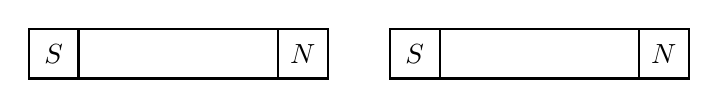
\begin{tikzpicture}[x=0.75pt,y=0.75pt,yscale=-0.6,xscale=0.6]
		%uncomment if require: \path (0,300); %set diagram left start at 0, and has height of 300

		%Shape: Rectangle [id:dp4379328648322769] 
		\draw   (100,110) -- (260,110) -- (260,150) -- (100,150) -- cycle ;
		%Shape: Rectangle [id:dp6350525414581176] 
		\draw   (260,110) -- (300,110) -- (300,150) -- (260,150) -- cycle ;
		%Shape: Rectangle [id:dp4096511233686948] 
		\draw   (60,110) -- (100,110) -- (100,150) -- (60,150) -- cycle ;
		%Shape: Rectangle [id:dp1736195095098798] 
		\draw   (390,110) -- (550,110) -- (550,150) -- (390,150) -- cycle ;
		%Shape: Rectangle [id:dp6389792905995233] 
		\draw   (550,110) -- (590,110) -- (590,150) -- (550,150) -- cycle ;
		%Shape: Rectangle [id:dp7014855427891589] 
		\draw   (350,110) -- (390,110) -- (390,150) -- (350,150) -- cycle ;

		% Text Node
		\draw (80,130) node    {$S$};
		% Text Node
		\draw (370,130) node    {$S$};
		% Text Node
		\draw (280,130) node    {$N$};
		% Text Node
		\draw (570,130) node    {$N$};

		\end{tikzpicture}
	\end{figure}
	\FloatBarrier

	Sebbene la struttura della formula sia identica a quella della forza fra due cariche elettriche, c'è una differenza fondamentale. \emph{Una carica elettrica, positiva o negativa, puo sempre essere isolata}; ciò è una conseguenza dell'esistenza della carica elementare positiva portata dal protone e della carica elementare negativa dell'elettrone, la possibilità di separazione esiste già a livello elementare. \emph{Non è invece mai stato possibile ottenere un polo magnetico isolato}. I poli magnetici sembrano esistere sempre a coppie di egual valore e segno opposto, si manifestano solamente sotto forma di dipoli magnetici. L'indicazione classica è costituita dall'esperimento della calamita spezzata. Se si taglia a meta la calamita compaiono sempre due poli di segno opposto nella zona del taglio, che precedentemente a questo non mostrava la proprietà di attirare la limatura di ferro.
\end{itemize}

La prima relazione tra fenomeni magnetici ed elettrici fu scoperta da Oersted nel 1811 e successivamente l'argomento venne approfondito soprattutto da Ampere intorno al 1820. La sperimentazione fu resa possibile dall'utilizzo della pila di Volta che, permettendo la produzione di correnti elettriche costanti e intense, aprì il campo dello studio dell'interazione tra circuiti percorsi da corrente e magneti. Oersted mostrò che un ago magnetico, posto in prossimità di un filo percorso da corrente, tende ad assumere una ben definita posizione di equilibrio. Alla luce di quanto visto finora il risultato si interpreta dicendo che il filo percorso da corrente produce un campo magnetico e che l'ago si orienta parallelamente al campo esistente nel punto in cui viene posto. In seguito Ampere dimostrò che anche due fili percorsi da corrente interagiscono e intuì che \emph{le azioni magnetiche non sono altro che la manifestazione dell'interazione tra cariche elettriche in movimento}. Egli nel 1827 pubblicò una teoria ancora oggi valida, affermante che le interazioni elettromagnetiche sono legate a correnti di tipo microscopico. Bisogna pensare che in ogni atomo o in ogni molecola devono esistere delle correnti microscopiche locali, che prendono il nome di correnti molecolari di Ampere o \emph{correnti amperiane}; l'interazione tra un circuito percorso da corrente e un magnete è allora risultato delle interazioni tra gli elettroni liberi in moto nel conduttore e le microcorrenti presenti nel materiale magnetizzato.

\textbf{Osservazione.} L'elettrone è puntiforme, per cui il momento magnetico appare proprio come una proprietà intrinseca, legata al momento angolare intrinseco (spin).

\section{Teorema di Gauss per il campo magnetico, III Equazione di Maxwell (anche in regime tempovariante)}

Per interpretare le interazioni di tipo magnetico si utilizza un approccio simile a quello usato per i campi elettrici. Considerato un filo percorso da corrente, esso genera attorno a sé una modifica delle proprietà dello spazio rappresentata da un campo vettoriale detto \emph{campo di induzione magnetica} $\vec{B}$.

\begin{figure}[htpb]
	\centering

	\tikzset{every picture/.style={line width=0.75pt}} %set default line width to 0.75pt        

	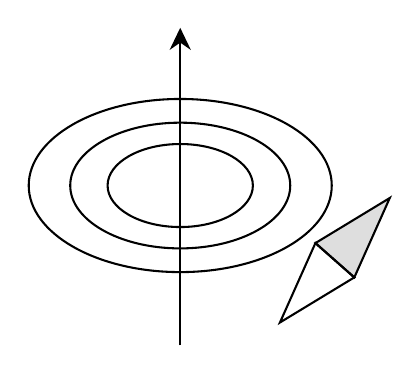
\begin{tikzpicture}[x=0.75pt,y=0.75pt,yscale=-1,xscale=1]
	%uncomment if require: \path (0,300); %set diagram left start at 0, and has height of 300

	%Straight Lines [id:da8308841647454677] 
	\draw    (179.5,228) -- (179.5,78) ;
	\draw [shift={(179.5,75)}, rotate = 450] [fill={rgb, 255:red, 0; green, 0; blue, 0 }  ][line width=0.08]  [draw opacity=0] (10.72,-5.15) -- (0,0) -- (10.72,5.15) -- (7.12,0) -- cycle    ;
	%Shape: Ellipse [id:dp5745765474173075] 
	\draw   (144.5,151) .. controls (144.5,139.95) and (160.17,131) .. (179.5,131) .. controls (198.83,131) and (214.5,139.95) .. (214.5,151) .. controls (214.5,162.05) and (198.83,171) .. (179.5,171) .. controls (160.17,171) and (144.5,162.05) .. (144.5,151) -- cycle ;
	%Shape: Triangle [id:dp08320703214712943] 
	\draw  [fill={rgb, 255:red, 222; green, 222; blue, 222 }  ,fill opacity=1 ] (280.46,157) -- (263.37,195.27) -- (244.63,178.73) -- cycle ;
	%Shape: Triangle [id:dp9261976129323173] 
	\draw   (227.54,217) -- (244.63,178.73) -- (263.37,195.27) -- cycle ;

	%Shape: Ellipse [id:dp20987696581529236] 
	\draw   (126.5,151) .. controls (126.5,134.27) and (150.23,120.71) .. (179.5,120.71) .. controls (208.77,120.71) and (232.5,134.27) .. (232.5,151) .. controls (232.5,167.73) and (208.77,181.29) .. (179.5,181.29) .. controls (150.23,181.29) and (126.5,167.73) .. (126.5,151) -- cycle ;
	%Shape: Ellipse [id:dp11041624129618621] 
	\draw   (106.5,151) .. controls (106.5,127.96) and (139.18,109.29) .. (179.5,109.29) .. controls (219.82,109.29) and (252.5,127.96) .. (252.5,151) .. controls (252.5,174.04) and (219.82,192.71) .. (179.5,192.71) .. controls (139.18,192.71) and (106.5,174.04) .. (106.5,151) -- cycle ;

	\end{tikzpicture}
\end{figure}
\FloatBarrier

Se vediamo che l'ago del magnete esploratore interagisce con il filo, lì è presente un campo magnetico. Per definire il campo magnetico in forma qualitativa si utilizza un ago magnetico. Nel caso dell'interazione fra campi elettrici e dipoli elettrici, quando un dipolo viene immerso in un campo $\vec{E}$ ruota in modo tale da rendere parallelo al campo il suo momento di dipolo. Una situazione analoga si ha con il campo magnetico. Si può studiare l'andamento di $\vec{B}$ con un piccolo ago magnetico: questo si orienta parallelamente a $\vec{B}$ indicandone cosi la direzione, mentre il verso è quello dal polo sud al polo nord dell'ago. Se esso è abbastanza piccolo si può supporre che $\vec{B}$ non vari lungo l'ago e quindi la misura sia effettivamente puntuale e non mediata.

Possiamo osservare che anche la legge di Coulomb magnetica ha una forza tale per cui l'interazione \emph{decresce con il quadrato della distanza ed è radiale}.

Questa è stata una condizione fondamentale per dimostrare il teorema di Gauss per il campo elettrico, quindi ci aspettiamo che \emph{anche per i campi magnetici valga un teorema di Gauss}. Siccome i magneti sono sempre composti da masse magnetiche opposte che non riusciamo a separare, qualunque superficie chiusa io prenda, all'interno avremo sempre lo stesso numero di masse positive e negative. \emph{Il flusso del campo magnetico attraverso una superficie chiusa sarà nullo}.

\begin{figure}[htpb]
	\centering

	% Pattern Info
	 
	\tikzset{
	pattern size/.store in=\mcSize, 
	pattern size = 5pt,
	pattern thickness/.store in=\mcThickness, 
	pattern thickness = 0.3pt,
	pattern radius/.store in=\mcRadius, 
	pattern radius = 1pt}
	\makeatletter
	\pgfutil@ifundefined{pgf@pattern@name@_1aq31xh1f}{
	\pgfdeclarepatternformonly[\mcThickness,\mcSize]{_1aq31xh1f}
	{\pgfqpoint{0pt}{0pt}}
	{\pgfpoint{\mcSize+\mcThickness}{\mcSize+\mcThickness}}
	{\pgfpoint{\mcSize}{\mcSize}}
	{
	\pgfsetcolor{\tikz@pattern@color}
	\pgfsetlinewidth{\mcThickness}
	\pgfpathmoveto{\pgfqpoint{0pt}{0pt}}
	\pgfpathlineto{\pgfpoint{\mcSize+\mcThickness}{\mcSize+\mcThickness}}
	\pgfusepath{stroke}
	}}
	\makeatother
	\tikzset{every picture/.style={line width=0.75pt}} %set default line width to 0.75pt        

	\begin{tikzpicture}[x=0.75pt,y=0.75pt,yscale=-1,xscale=1]
	%uncomment if require: \path (0,300); %set diagram left start at 0, and has height of 300

	%Shape: Ellipse [id:dp9222605722816104] 
	\draw  [pattern=_1aq31xh1f,pattern size=6pt,pattern thickness=0.75pt,pattern radius=0pt, pattern color={rgb, 255:red, 222; green, 222; blue, 222}] (214.01,99.16) .. controls (214.01,65.28) and (241.47,37.81) .. (275.36,37.81) .. controls (309.24,37.81) and (336.71,65.28) .. (336.71,99.16) .. controls (336.71,133.04) and (309.24,160.51) .. (275.36,160.51) .. controls (241.47,160.51) and (214.01,133.04) .. (214.01,99.16) -- cycle ;
	%Shape: Ellipse [id:dp4016085591912175] 
	\draw   (246.68,158.33) .. controls (246.68,142.29) and (269.43,129.29) .. (297.5,129.29) .. controls (325.57,129.29) and (348.32,142.29) .. (348.32,158.33) .. controls (348.32,174.37) and (325.57,187.37) .. (297.5,187.37) .. controls (269.43,187.37) and (246.68,174.37) .. (246.68,158.33) -- cycle ;
	%Shape: Ellipse [id:dp36375410760407245] 
	\draw   (220.54,158.33) .. controls (220.54,134.04) and (255,114.36) .. (297.5,114.36) .. controls (340,114.36) and (374.46,134.04) .. (374.46,158.33) .. controls (374.46,182.62) and (340,202.31) .. (297.5,202.31) .. controls (255,202.31) and (220.54,182.62) .. (220.54,158.33) -- cycle ;
	%Shape: Ellipse [id:dp8010793881307494] 
	\draw   (191.5,158.33) .. controls (191.5,124.88) and (238.96,97.76) .. (297.5,97.76) .. controls (356.04,97.76) and (403.5,124.88) .. (403.5,158.33) .. controls (403.5,191.78) and (356.04,218.9) .. (297.5,218.9) .. controls (238.96,218.9) and (191.5,191.78) .. (191.5,158.33) -- cycle ;
	\draw   (286.75,180.75) -- (300.25,187.5) -- (286.75,194.25) ;
	\draw   (302.25,194.25) -- (315.75,201) -- (302.25,207.75) ;
	\draw   (281.25,211.75) -- (294.75,218.5) -- (281.25,225.25) ;

	% Text Node
	\draw (210.5,53.5) node    {$\Sigma _{g}$};
	% Text Node
	\draw (414,150) node    {$\vec{B}$};

	\end{tikzpicture}
\end{figure}
\FloatBarrier

Possiamo a questo punto ricavare la \textbf{III Equazione di Maxwell} applicando il teorema della Divergenza.

\[
	\Phi_{\Sigma}(\vec{B}) = \int_{\Sigma}\vec{B} \cdot \vec{n} dS = \int_{\tau} \text{div}\vec{B} \, d\tau  = 0
\]

Quindi la divergenza di $\vec{B}$ è sempre nulla in tutti i punti dello spazio.

\[
	\text{div}\vec{B} =0
\]

Questa equazione vale in qualsiasi regime, sia stazionario che tempovariante. Quando un campo vettoriale ha divergenza pari a zero ovunque, esso viene chiamato \emph{solenoidale}. Quindi il campo magnetico è un campo solenoidale. Siccome la divergenza ci dice dove sono le sorgenti di flusso, per questo particolare campo vettoriale non ci sono sorgenti positive o negative, \emph{le linee di flusso sono chiuse}.

\begin{figure}[htpb]
	\centering

	\tikzset{every picture/.style={line width=0.75pt}} %set default line width to 0.75pt        

	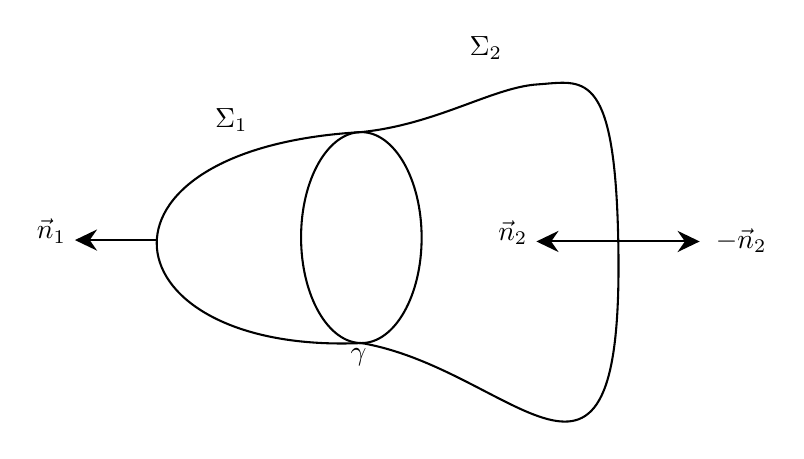
\begin{tikzpicture}[x=0.75pt,y=0.75pt,yscale=-1,xscale=1]
	%uncomment if require: \path (0,300); %set diagram left start at 0, and has height of 300

	%Shape: Ellipse [id:dp4993447536693967] 
	\draw   (276.73,187.62) .. controls (260.7,187.65) and (247.66,164.91) .. (247.61,136.84) .. controls (247.57,108.78) and (260.54,86) .. (276.57,85.98) .. controls (292.61,85.95) and (305.65,108.69) .. (305.7,136.75) .. controls (305.74,164.82) and (292.77,187.6) .. (276.73,187.62) -- cycle ;
	%Curve Lines [id:da3193485518740673] 
	\draw    (276.73,187.62) .. controls (153.41,192.99) and (137.26,94.02) .. (276.57,85.98) ;
	%Curve Lines [id:da3253006873399502] 
	\draw    (276.73,187.62) .. controls (314.58,194.15) and (346.54,220.14) .. (368.5,224.76) .. controls (390.47,229.37) and (402.44,212.6) .. (400.32,133.6) .. controls (398.19,54.61) and (383.1,61.57) .. (361.5,63) .. controls (339.9,64.43) and (312.9,82.33) .. (276.57,85.98) ;
	%Straight Lines [id:da29819932081250955] 
	\draw    (178,138) -- (141.67,138) ;
	\draw [shift={(138.67,138)}, rotate = 360] [fill={rgb, 255:red, 0; green, 0; blue, 0 }  ][line width=0.08]  [draw opacity=0] (10.72,-5.15) -- (0,0) -- (10.72,5.15) -- (7.12,0) -- cycle    ;
	%Straight Lines [id:da5245812337382556] 
	\draw    (400.33,138.67) -- (364,138.67) ;
	\draw [shift={(361,138.67)}, rotate = 360] [fill={rgb, 255:red, 0; green, 0; blue, 0 }  ][line width=0.08]  [draw opacity=0] (10.72,-5.15) -- (0,0) -- (10.72,5.15) -- (7.12,0) -- cycle    ;
	%Straight Lines [id:da542773982948495] 
	\draw    (436.67,138.67) -- (400.33,138.67) ;
	\draw [shift={(439.67,138.67)}, rotate = 180] [fill={rgb, 255:red, 0; green, 0; blue, 0 }  ][line width=0.08]  [draw opacity=0] (10.72,-5.15) -- (0,0) -- (10.72,5.15) -- (7.12,0) -- cycle    ;

	% Text Node
	\draw (275.33,194.33) node    {$\gamma $};
	% Text Node
	\draw (214,80.33) node    {$\Sigma _{1}$};
	% Text Node
	\draw (336.67,45.67) node    {$\Sigma _{2}$};
	% Text Node
	\draw (127.33,133.67) node    {$\vec{n}_{1}$};
	% Text Node
	\draw (349.67,134.33) node    {$\vec{n}_{2}$};
	% Text Node
	\draw (459.67,138.33) node    {$-\vec{n}_{2}$};

	\end{tikzpicture}
\end{figure}
\FloatBarrier

Immaginiamo di considerare una linea chiusa $\gamma$ su cui è costruita una superficie aperta $\Sigma_1$ e una $\Sigma_2$. Dato che sono due superfici aperte, possiamo scegliere la normale $\vec{n}$ come vogliamo. Immaginiamo che in questa regione dello spazio ci sia un campo magnetico. L'insieme delle due superfici è una superficie chiusa. Chiamiamo $\Sigma$ la loro unione.

\begin{equation*}
	\begin{aligned}
		\Phi_{\Sigma} (\vec{B} ) = 0 &= \int_{\Sigma_1}\vec{B} \cdot \vec{n}_1  dS + \int_{\Sigma_2}\vec{B} \cdot (-\vec{n}_2)dS \\
		&= \underbrace{\int_{\Sigma_1}\vec{B} \cdot \vec{n}_1  dS}_{\Phi_{\Sigma_1}(\vec{B} )}  - \underbrace{\int_{\Sigma_2}\vec{B} \cdot \vec{n}_1 dS}_{\Phi_{\Sigma_2}(\vec{B} )}  \implies \Phi_{\Sigma_1}(\vec{B} ) = \Phi_{\Sigma_2}(\vec{B} )
	\end{aligned}
\end{equation*}

Quindi considerata una linea chiusa $\gamma$, qualunque superficie che abbia tale linea come contorno avrà lo stesso flusso di $\vec{B}$.
Possiamo chiamare questo flusso: \emph{flusso del campo magnetico concatenato a} $\gamma$.

\section{Forza di Lorentz}

Abbiamo detto che i campi magnetici sono prodotti da cariche in moto che agiscono su altre cariche in moto. Possiamo immaginare come sonda nella regione di spazio in cui è presente un campo $\vec{B}$ una carica in moto.
Si verifica sperimentalmente che sulla carica agisce una forza pari a:

\[
	\boxed{\vec{F} = q\vec{v} \times \vec{B}}
\]

La prima proprietà da osservare è che se la velocità della carica
è zero la forza di Lorentz è pari a zero. Infatti le forze magnetiche agiscono fra cariche in moto. Se la carica è in quiete non c'è alcuna forza che agisce su di essa. Supponiamo di trovarci su un altro sistema di riferimento inerziale che viaggia ad una certa velocità. In tale sistema di riferimento vedo la carica in moto. Sembrerebbe che questa formula dipenda dal sistema di riferimento su cui si trova la carica.

\begin{figure}[htpb]
	\centering

	\tikzset{every picture/.style={line width=0.75pt}} %set default line width to 0.75pt        

	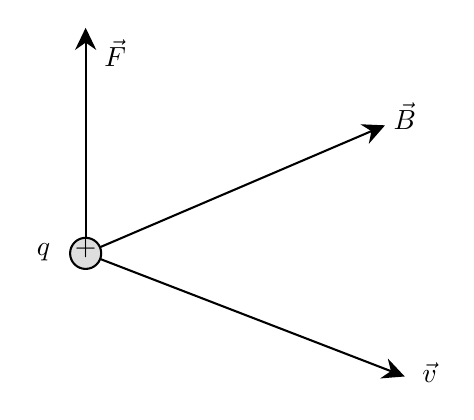
\begin{tikzpicture}[x=0.75pt,y=0.75pt,yscale=-1,xscale=1]
	%uncomment if require: \path (0,300); %set diagram left start at 0, and has height of 300

	%Straight Lines [id:da24951894038501976] 
	\draw    (407.7,221.67) -- (256.77,163.43) ;
	\draw [shift={(410.5,222.75)}, rotate = 201.1] [fill={rgb, 255:red, 0; green, 0; blue, 0 }  ][line width=0.08]  [draw opacity=0] (10.72,-5.15) -- (0,0) -- (10.72,5.15) -- (7.12,0) -- cycle    ;
	%Straight Lines [id:da5487854509807417] 
	\draw    (398.24,102.93) -- (256.77,163.43) ;
	\draw [shift={(401,101.75)}, rotate = 156.85] [fill={rgb, 255:red, 0; green, 0; blue, 0 }  ][line width=0.08]  [draw opacity=0] (10.72,-5.15) -- (0,0) -- (10.72,5.15) -- (7.12,0) -- cycle    ;
	%Straight Lines [id:da24462379929793854] 
	\draw    (256.77,57.75) -- (256.77,163.43) ;
	\draw [shift={(256.77,54.75)}, rotate = 90] [fill={rgb, 255:red, 0; green, 0; blue, 0 }  ][line width=0.08]  [draw opacity=0] (10.72,-5.15) -- (0,0) -- (10.72,5.15) -- (7.12,0) -- cycle    ;
	%Shape: Circle [id:dp3064944724065122] 
	\draw  [fill={rgb, 255:red, 222; green, 222; blue, 222 }  ,fill opacity=1 ] (249.27,163.43) .. controls (249.27,159.29) and (252.62,155.93) .. (256.77,155.93) .. controls (260.91,155.93) and (264.27,159.29) .. (264.27,163.43) .. controls (264.27,167.58) and (260.91,170.93) .. (256.77,170.93) .. controls (252.62,170.93) and (249.27,167.58) .. (249.27,163.43) -- cycle ;

	% Text Node
	\draw (256.77,160.93) node    {$+$};
	% Text Node
	\draw (410.5,97.5) node    {$\vec{B}$};
	% Text Node
	\draw (422.5,221) node    {$\vec{v}$};
	% Text Node
	\draw (271,67) node    {$\vec{F}$};
	% Text Node
	\draw (236.5,163) node    {$q$};

	\end{tikzpicture}
\end{figure}
\FloatBarrier

Se la velocità non è nulla ma è parallela a $\vec{B}$, la forza è zero. Se la velocità è perpendicolare a $\vec{B}$ il modulo della forza è massimo. Comunque $\vec{F}$ è sempre perpendicolare a $\vec{v}$. Abbiamo definitivo la potenza dissipata dalla forza come:

\[
	w=\vec{F} \cdot \vec{v} = 0
\]

Tale prodotto scalare diventa allora zero. Significa che la forza di Lorentz non dissipa potenza, ovvero, se consideriamo la nostra carica in moto in presenza di campo magnetico, la forza sarà fatta come in figura.
Se calcoliamo il lavoro compiuto dalla forza infinitesima:

\[
	\mathcal{L}_{AB}=\int_A^B \vec{F} \cdot d\vec{l} =0 \implies \Delta K=0
\]

Il modulo della velocità rimane quindi costante perché $\Delta K$ dipende dal quadrato della velocità, ma non vi è una sua variazione del tempo. Segue che il moto di una carica in un campo magnetico è uniforme. A parità di intensità del campo magnetico, la carica negativa e la carica positiva subiranno forze in versi opposti. Il campo magnetico in un punto è definito come quel vettore tale per cui la forza agente sulla carica in tal punto è pari alla forza di Lorentz.

\[
	|\vec{v} |=v_s = \text{costante}
\]

Dimensionalmente abbiamo

\[
	[F]=\frac{[Q][L]}{[T]}\cdot [B] \qquad \implies [B]=\frac{[F][T]}{[Q][L]}
\]

\[
	\left( \frac{N}{C}\cdot \frac{S}{m} \right) =\left( \frac{V}{m}\cdot \frac{S}{m} \right) = \left( \frac{V\cdot S}{m^2} \right) = \left( \frac{Wb}{m^2}\right)=T
\]

Con $ T =$ Tesla e $ Wb= $ Weber.

Il tesla è una unità di misura sovra-dimensionata. Sulla superficie terrestre, il valore del campo varia in intensità, dall'equatore ai poli, da circa $ 20000 nT $ a $ 70000 nT $.
Si definisce quindi il Gauss: $ 1 G = 10^{-4} T $

\section{Moto di una carica in un campo magnetico uniforme}

Consideriamo una carica in moto in una regione in cui è presente un campo magnetico $\vec{B}$, con velocità $\vec{v}$ perpendicolare a $ \vec{B}$. L'unica forza che agisce è quella di Lorentz. La deviazione della direzione della velocità avviene sul piano.

\[
	\vec{F} = q\vec{v} \times \vec{B}
\]

\begin{figure}[htpb]
	\centering

	\tikzset{every picture/.style={line width=0.75pt}} %set default line width to 0.75pt        

	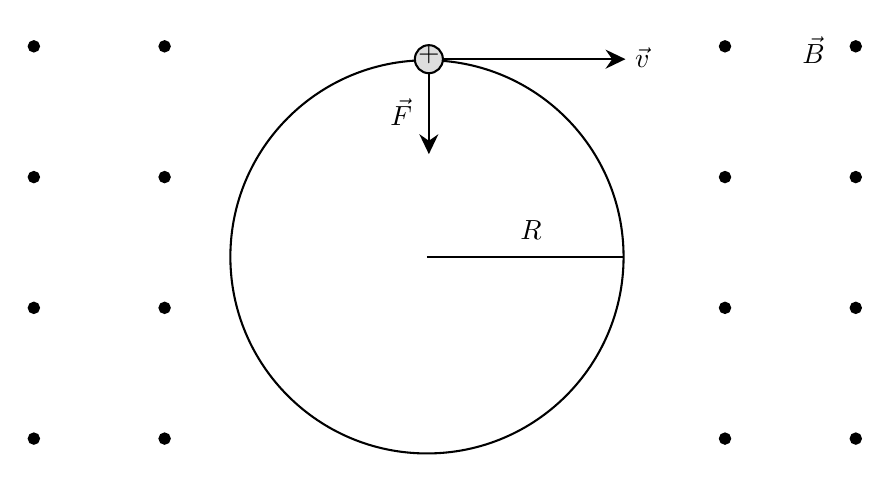
\begin{tikzpicture}[x=0.75pt,y=0.75pt,yscale=-0.9,xscale=0.9]
	%uncomment if require: \path (0,300); %set diagram left start at 0, and has height of 300

	%Shape: Circle [id:dp23188527005327408] 
	\draw  [fill={rgb, 255:red, 0; green, 0; blue, 0 }  ,fill opacity=1 ] (186.05,29.55) .. controls (186.05,28.03) and (187.28,26.8) .. (188.8,26.8) .. controls (190.32,26.8) and (191.55,28.03) .. (191.55,29.55) .. controls (191.55,31.07) and (190.32,32.3) .. (188.8,32.3) .. controls (187.28,32.3) and (186.05,31.07) .. (186.05,29.55) -- cycle ;
	%Shape: Circle [id:dp3151248833710725] 
	\draw  [fill={rgb, 255:red, 0; green, 0; blue, 0 }  ,fill opacity=1 ] (186.05,99.55) .. controls (186.05,98.03) and (187.28,96.8) .. (188.8,96.8) .. controls (190.32,96.8) and (191.55,98.03) .. (191.55,99.55) .. controls (191.55,101.07) and (190.32,102.3) .. (188.8,102.3) .. controls (187.28,102.3) and (186.05,101.07) .. (186.05,99.55) -- cycle ;
	%Shape: Circle [id:dp33386804817308025] 
	\draw  [fill={rgb, 255:red, 0; green, 0; blue, 0 }  ,fill opacity=1 ] (186.05,169.55) .. controls (186.05,168.03) and (187.28,166.8) .. (188.8,166.8) .. controls (190.32,166.8) and (191.55,168.03) .. (191.55,169.55) .. controls (191.55,171.07) and (190.32,172.3) .. (188.8,172.3) .. controls (187.28,172.3) and (186.05,171.07) .. (186.05,169.55) -- cycle ;
	%Shape: Circle [id:dp7042195434142586] 
	\draw  [fill={rgb, 255:red, 0; green, 0; blue, 0 }  ,fill opacity=1 ] (186.05,239.55) .. controls (186.05,238.03) and (187.28,236.8) .. (188.8,236.8) .. controls (190.32,236.8) and (191.55,238.03) .. (191.55,239.55) .. controls (191.55,241.07) and (190.32,242.3) .. (188.8,242.3) .. controls (187.28,242.3) and (186.05,241.07) .. (186.05,239.55) -- cycle ;
	%Shape: Circle [id:dp6237047411495382] 
	\draw   (224,142.25) .. controls (224,84.12) and (271.12,37) .. (329.25,37) .. controls (387.38,37) and (434.5,84.12) .. (434.5,142.25) .. controls (434.5,200.38) and (387.38,247.5) .. (329.25,247.5) .. controls (271.12,247.5) and (224,200.38) .. (224,142.25) -- cycle ;
	%Straight Lines [id:da6231155453525645] 
	\draw    (329.25,142.25) -- (434.5,142.25) ;
	%Straight Lines [id:da6167820082823245] 
	\draw    (330.27,36.43) -- (432.52,36.43) ;
	\draw [shift={(435.52,36.43)}, rotate = 180] [fill={rgb, 255:red, 0; green, 0; blue, 0 }  ][line width=0.08]  [draw opacity=0] (10.72,-5.15) -- (0,0) -- (10.72,5.15) -- (7.12,0) -- cycle    ;
	%Straight Lines [id:da571191659258169] 
	\draw    (330.27,36.43) -- (330.27,84.25) ;
	\draw [shift={(330.27,87.25)}, rotate = 270] [fill={rgb, 255:red, 0; green, 0; blue, 0 }  ][line width=0.08]  [draw opacity=0] (10.72,-5.15) -- (0,0) -- (10.72,5.15) -- (7.12,0) -- cycle    ;
	%Shape: Circle [id:dp01683522605612775] 
	\draw  [fill={rgb, 255:red, 222; green, 222; blue, 222 }  ,fill opacity=1 ] (322.77,36.43) .. controls (322.77,32.29) and (326.12,28.93) .. (330.27,28.93) .. controls (334.41,28.93) and (337.77,32.29) .. (337.77,36.43) .. controls (337.77,40.58) and (334.41,43.93) .. (330.27,43.93) .. controls (326.12,43.93) and (322.77,40.58) .. (322.77,36.43) -- cycle ;

	%Shape: Circle [id:dp5265854373631442] 
	\draw  [fill={rgb, 255:red, 0; green, 0; blue, 0 }  ,fill opacity=1 ] (116.05,29.55) .. controls (116.05,28.03) and (117.28,26.8) .. (118.8,26.8) .. controls (120.32,26.8) and (121.55,28.03) .. (121.55,29.55) .. controls (121.55,31.07) and (120.32,32.3) .. (118.8,32.3) .. controls (117.28,32.3) and (116.05,31.07) .. (116.05,29.55) -- cycle ;
	%Shape: Circle [id:dp35288825789599043] 
	\draw  [fill={rgb, 255:red, 0; green, 0; blue, 0 }  ,fill opacity=1 ] (116.05,99.55) .. controls (116.05,98.03) and (117.28,96.8) .. (118.8,96.8) .. controls (120.32,96.8) and (121.55,98.03) .. (121.55,99.55) .. controls (121.55,101.07) and (120.32,102.3) .. (118.8,102.3) .. controls (117.28,102.3) and (116.05,101.07) .. (116.05,99.55) -- cycle ;
	%Shape: Circle [id:dp8684657825124835] 
	\draw  [fill={rgb, 255:red, 0; green, 0; blue, 0 }  ,fill opacity=1 ] (116.05,169.55) .. controls (116.05,168.03) and (117.28,166.8) .. (118.8,166.8) .. controls (120.32,166.8) and (121.55,168.03) .. (121.55,169.55) .. controls (121.55,171.07) and (120.32,172.3) .. (118.8,172.3) .. controls (117.28,172.3) and (116.05,171.07) .. (116.05,169.55) -- cycle ;
	%Shape: Circle [id:dp7100765936828766] 
	\draw  [fill={rgb, 255:red, 0; green, 0; blue, 0 }  ,fill opacity=1 ] (116.05,239.55) .. controls (116.05,238.03) and (117.28,236.8) .. (118.8,236.8) .. controls (120.32,236.8) and (121.55,238.03) .. (121.55,239.55) .. controls (121.55,241.07) and (120.32,242.3) .. (118.8,242.3) .. controls (117.28,242.3) and (116.05,241.07) .. (116.05,239.55) -- cycle ;
	%Shape: Circle [id:dp3104752082490132] 
	\draw  [fill={rgb, 255:red, 0; green, 0; blue, 0 }  ,fill opacity=1 ] (556.05,29.55) .. controls (556.05,28.03) and (557.28,26.8) .. (558.8,26.8) .. controls (560.32,26.8) and (561.55,28.03) .. (561.55,29.55) .. controls (561.55,31.07) and (560.32,32.3) .. (558.8,32.3) .. controls (557.28,32.3) and (556.05,31.07) .. (556.05,29.55) -- cycle ;
	%Shape: Circle [id:dp24861452344507984] 
	\draw  [fill={rgb, 255:red, 0; green, 0; blue, 0 }  ,fill opacity=1 ] (556.05,99.55) .. controls (556.05,98.03) and (557.28,96.8) .. (558.8,96.8) .. controls (560.32,96.8) and (561.55,98.03) .. (561.55,99.55) .. controls (561.55,101.07) and (560.32,102.3) .. (558.8,102.3) .. controls (557.28,102.3) and (556.05,101.07) .. (556.05,99.55) -- cycle ;
	%Shape: Circle [id:dp8507140470140022] 
	\draw  [fill={rgb, 255:red, 0; green, 0; blue, 0 }  ,fill opacity=1 ] (556.05,169.55) .. controls (556.05,168.03) and (557.28,166.8) .. (558.8,166.8) .. controls (560.32,166.8) and (561.55,168.03) .. (561.55,169.55) .. controls (561.55,171.07) and (560.32,172.3) .. (558.8,172.3) .. controls (557.28,172.3) and (556.05,171.07) .. (556.05,169.55) -- cycle ;
	%Shape: Circle [id:dp8349390271245463] 
	\draw  [fill={rgb, 255:red, 0; green, 0; blue, 0 }  ,fill opacity=1 ] (556.05,239.55) .. controls (556.05,238.03) and (557.28,236.8) .. (558.8,236.8) .. controls (560.32,236.8) and (561.55,238.03) .. (561.55,239.55) .. controls (561.55,241.07) and (560.32,242.3) .. (558.8,242.3) .. controls (557.28,242.3) and (556.05,241.07) .. (556.05,239.55) -- cycle ;
	%Shape: Circle [id:dp7166248238687152] 
	\draw  [fill={rgb, 255:red, 0; green, 0; blue, 0 }  ,fill opacity=1 ] (486.05,29.55) .. controls (486.05,28.03) and (487.28,26.8) .. (488.8,26.8) .. controls (490.32,26.8) and (491.55,28.03) .. (491.55,29.55) .. controls (491.55,31.07) and (490.32,32.3) .. (488.8,32.3) .. controls (487.28,32.3) and (486.05,31.07) .. (486.05,29.55) -- cycle ;
	%Shape: Circle [id:dp05061953433231636] 
	\draw  [fill={rgb, 255:red, 0; green, 0; blue, 0 }  ,fill opacity=1 ] (486.05,99.55) .. controls (486.05,98.03) and (487.28,96.8) .. (488.8,96.8) .. controls (490.32,96.8) and (491.55,98.03) .. (491.55,99.55) .. controls (491.55,101.07) and (490.32,102.3) .. (488.8,102.3) .. controls (487.28,102.3) and (486.05,101.07) .. (486.05,99.55) -- cycle ;
	%Shape: Circle [id:dp7111663881487575] 
	\draw  [fill={rgb, 255:red, 0; green, 0; blue, 0 }  ,fill opacity=1 ] (486.05,169.55) .. controls (486.05,168.03) and (487.28,166.8) .. (488.8,166.8) .. controls (490.32,166.8) and (491.55,168.03) .. (491.55,169.55) .. controls (491.55,171.07) and (490.32,172.3) .. (488.8,172.3) .. controls (487.28,172.3) and (486.05,171.07) .. (486.05,169.55) -- cycle ;
	%Shape: Circle [id:dp9560662872299377] 
	\draw  [fill={rgb, 255:red, 0; green, 0; blue, 0 }  ,fill opacity=1 ] (486.05,239.55) .. controls (486.05,238.03) and (487.28,236.8) .. (488.8,236.8) .. controls (490.32,236.8) and (491.55,238.03) .. (491.55,239.55) .. controls (491.55,241.07) and (490.32,242.3) .. (488.8,242.3) .. controls (487.28,242.3) and (486.05,241.07) .. (486.05,239.55) -- cycle ;

	% Text Node
	\draw (330.27,33.93) node    {$+$};
	% Text Node
	\draw (385,128) node    {$R$};
	% Text Node
	\draw (315.5,65) node    {$\vec{F}$};
	% Text Node
	\draw (444.5,35.5) node    {$\vec{v}$};
	% Text Node
	\draw (536.17,31.67) node    {$\vec{B}$};

	\end{tikzpicture}
\end{figure}
\FloatBarrier

Il modulo della forza è costante del tempo. Si tratta di un moto circolare uniforme, di cui si osservano tutte le proprietà caratteristiche. Possiamo definire il raggio $ R $ della traiettoria e provare a stabilire un legame fra $ R $ e la forza, che possiamo pensare come centripeta (diretta verso il centro)

\[
	\vec{F} =m\vec{a}_c \qquad |\vec{F} |=m a_c=\frac{mv^2}{R}=qvB \implies \boxed{R=\frac{mv}{qB}}
\]

Ricordiamo ora dalla Fisica I la seguente relazione vettoriale

\[
	\vec{a}_c=\vec{\omega} \times \vec{v}
\]

Pertanto avremo, sostituendo nelle relazioni precedenti:

\begin{equation*}
	\begin{aligned}
		\vec{F} =q\vec{v} \times \vec{B} &= m\vec{a}_c \\
		\vec{v} \times q\vec{B}  &= m\vec{\omega} \times \vec{v} \\
		\vec{v} \times q\vec{B}  &=\vec{v} \times (-m\vec{\omega} )
	\end{aligned}
\end{equation*}

Dove è stata applicata la proprietà anticommutativa del prodotto vettoriale, infine abbiamo

\[
	q\vec{B} = -m\vec{\omega} \implies \boxed{\vec{\omega} = -\frac{q\vec{B}}{m}}
\]

Vettorialmente vediamo quindi che $ \omega $ è sempre opposta a $\vec{B}$.

Nel caso in cui $\vec{v}$ non sia ortogonale al campo ma formi un certo angolo $\vartheta$ con esso dovremo considerare la componente perpendicolare.

\[
	\vec{F} =q(\vec{v}_{\parallel}+\vec{v}_{\bot})\times \vec{B} = q\vec{v}_{\bot}\times \vec{B}
\]

\begin{figure}[htpb]
	\centering

	\tikzset{every picture/.style={line width=0.75pt}} %set default line width to 0.75pt        

	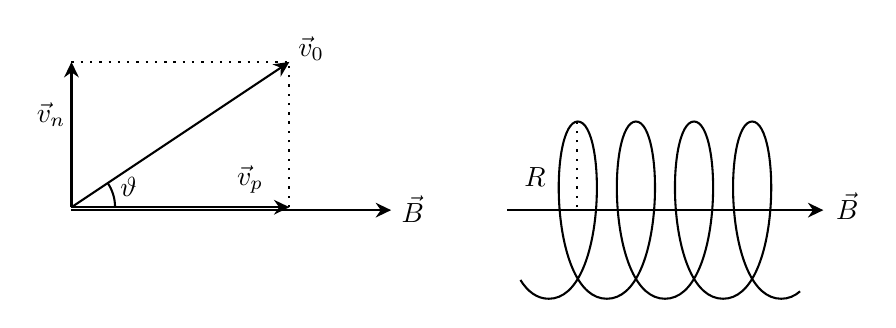
\begin{tikzpicture}[x=0.75pt,y=0.75pt,yscale=-0.7,xscale=0.7]
	%uncomment if require: \path (0,300); %set diagram left start at 0, and has height of 300

	%Shape: Spring [id:dp9279391676836501] 
	\draw  [color={rgb, 255:red, 0; green, 0; blue, 0 }  ,draw opacity=1 ] (345,250.09) .. controls (349.98,258.03) and (356.42,263) .. (364.5,263) .. controls (404.5,263) and (404.5,141) .. (384.5,141) .. controls (364.5,141) and (364.5,263) .. (404.5,263) .. controls (444.5,263) and (444.5,141) .. (424.5,141) .. controls (404.5,141) and (404.5,263) .. (444.5,263) .. controls (484.5,263) and (484.5,141) .. (464.5,141) .. controls (444.5,141) and (444.5,263) .. (484.5,263) .. controls (524.5,263) and (524.5,141) .. (504.5,141) .. controls (484.5,141) and (484.5,263) .. (524.5,263) .. controls (529.43,263) and (533.75,261.15) .. (537.5,257.9) ;
	%Straight Lines [id:da7085363059097909] 
	\draw    (36,200) -- (183,200) ;
	\draw [shift={(186,200)}, rotate = 180] [fill={rgb, 255:red, 0; green, 0; blue, 0 }  ][line width=0.08]  [draw opacity=0] (10.72,-5.15) -- (0,0) -- (10.72,5.15) -- (7.12,0) -- cycle    ;
	%Straight Lines [id:da8596236417176182] 
	\draw    (36,200) -- (183.5,101.66) ;
	\draw [shift={(186,100)}, rotate = 506.31] [fill={rgb, 255:red, 0; green, 0; blue, 0 }  ][line width=0.08]  [draw opacity=0] (10.72,-5.15) -- (0,0) -- (10.72,5.15) -- (7.12,0) -- cycle    ;
	%Straight Lines [id:da4245362862630413] 
	\draw    (36,200) -- (36,103) ;
	\draw [shift={(36,100)}, rotate = 450] [fill={rgb, 255:red, 0; green, 0; blue, 0 }  ][line width=0.08]  [draw opacity=0] (10.72,-5.15) -- (0,0) -- (10.72,5.15) -- (7.12,0) -- cycle    ;
	%Straight Lines [id:da5299214536869359] 
	\draw  [dash pattern={on 0.84pt off 2.51pt}]  (36,100) -- (186,100) ;
	%Straight Lines [id:da31044452089539964] 
	\draw  [dash pattern={on 0.84pt off 2.51pt}]  (186,200) -- (186,100) ;
	%Straight Lines [id:da3319296169460262] 
	\draw    (36,202) -- (253,202) ;
	\draw [shift={(256,202)}, rotate = 180] [fill={rgb, 255:red, 0; green, 0; blue, 0 }  ][line width=0.08]  [draw opacity=0] (10.72,-5.15) -- (0,0) -- (10.72,5.15) -- (7.12,0) -- cycle    ;
	%Shape: Arc [id:dp7996534054265312] 
	\draw  [draw opacity=0] (60.86,183.21) .. controls (64.09,187.97) and (65.98,193.71) .. (66,199.89) -- (36,200) -- cycle ; \draw   (60.86,183.21) .. controls (64.09,187.97) and (65.98,193.71) .. (66,199.89) ;
	%Straight Lines [id:da0474297745656187] 
	\draw  [dash pattern={on 0.84pt off 2.51pt}]  (384,200) -- (384,141.33) ;
	%Straight Lines [id:da9478959187866598] 
	\draw    (336,202) -- (550.5,202) ;
	\draw [shift={(553.5,202)}, rotate = 180] [fill={rgb, 255:red, 0; green, 0; blue, 0 }  ][line width=0.08]  [draw opacity=0] (10.72,-5.15) -- (0,0) -- (10.72,5.15) -- (7.12,0) -- cycle    ;

	% Text Node
	\draw (159,181) node    {$\vec{v}_{p}$};
	% Text Node
	\draw (22,136) node    {$\vec{v}_{n}$};
	% Text Node
	\draw (201,91) node    {$\vec{v}_{0}$};
	% Text Node
	\draw (271,201) node    {$\vec{B}$};
	% Text Node
	\draw (75.33,186) node    {$\vartheta $};
	% Text Node
	\draw (355,179) node    {$R$};
	% Text Node
	\draw (570,199.33) node    {$\vec{B}$};

	\end{tikzpicture}
\end{figure}
\FloatBarrier

Abbiamo quindi la composizione del moto circolare uniforme in un piano ortogonale a $\vec{B}$ e del moto circolare uniforme lungo $\vec{B}$, che è un moto elicoidale uniforme avente come asse la direzione di $\vec{B}$. Nel tempo la particella si sposta lungo $\vec{B}$ della quantità:

\[
	p=v_{\parallel}\, t= \frac{2\pi mv\cos \vartheta}{qB}
\]

detto \emph{passo dell'elica}.

\section{Forza magnetica agente su conduttori percorsi da corrente (II legge di Laplace)}

Se consideriamo il caso di un conduttore in cui fluisce corrente, avremo delle cariche in moto all'interno di esso. Che cosa accade se espongo il conduttore percorso da corrente ad un campo magnetico? Ciascuna delle cariche in moto subirà una forza di Lorentz. Il moto delle cariche è molto complesso: caotico sovrapposto a un moto di deriva. Se calcoliamo il valor medio della forza di Lorentz agente sulla singola carica avremo:

\[
	\langle \vec{F} \rangle = q\vec{v}_d\times \vec{B}
\]

\begin{figure}[htpb]
	\centering

	\tikzset{every picture/.style={line width=0.75pt}} %set default line width to 0.75pt        

	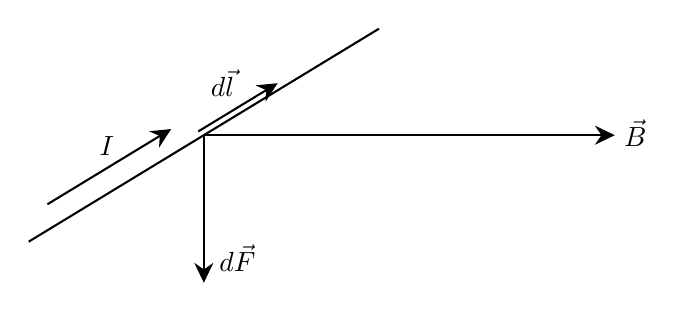
\begin{tikzpicture}[x=0.75pt,y=0.75pt,yscale=-0.9,xscale=0.9]
	%uncomment if require: \path (0,300); %set diagram left start at 0, and has height of 300

	%Straight Lines [id:da7320324873567214] 
	\draw    (332.75,76) -- (145.25,190) ;
	%Straight Lines [id:da5802726838205565] 
	\draw    (239,133) -- (456,133) ;
	\draw [shift={(459,133)}, rotate = 180] [fill={rgb, 255:red, 0; green, 0; blue, 0 }  ][line width=0.08]  [draw opacity=0] (10.72,-5.15) -- (0,0) -- (10.72,5.15) -- (7.12,0) -- cycle    ;
	%Straight Lines [id:da4587584641746505] 
	\draw    (218.94,131.28) -- (155.25,170) ;
	\draw [shift={(221.5,129.72)}, rotate = 148.7] [fill={rgb, 255:red, 0; green, 0; blue, 0 }  ][line width=0.08]  [draw opacity=0] (10.72,-5.15) -- (0,0) -- (10.72,5.15) -- (7.12,0) -- cycle    ;
	%Straight Lines [id:da8949125682974581] 
	\draw    (275.94,106.72) -- (236,131) ;
	\draw [shift={(278.5,105.16)}, rotate = 148.7] [fill={rgb, 255:red, 0; green, 0; blue, 0 }  ][line width=0.08]  [draw opacity=0] (10.72,-5.15) -- (0,0) -- (10.72,5.15) -- (7.12,0) -- cycle    ;
	%Straight Lines [id:da667896447295699] 
	\draw    (239,133) -- (239,209) ;
	\draw [shift={(239,212)}, rotate = 270] [fill={rgb, 255:red, 0; green, 0; blue, 0 }  ][line width=0.08]  [draw opacity=0] (10.72,-5.15) -- (0,0) -- (10.72,5.15) -- (7.12,0) -- cycle    ;

	% Text Node
	\draw (470,132) node    {$\vec{B}$};
	% Text Node
	\draw (187,139) node    {$I$};
	% Text Node
	\draw (249,105) node    {$d\vec{l}$};
	% Text Node
	\draw (257,199) node    {$d\vec{F}$};

	\end{tikzpicture}
\end{figure}
\FloatBarrier

Consideriamo un tratto $dl$ di lunghezza infinitesima sul nostro conduttore, parallelo alla superficie del conduttore e diretto nel verso in cui scorre la corrente. Consideriamo anche il volume di conduttore $ d\tau$, avremo:

\[
	d\vec{F} = \langle \vec{F} \rangle n \, d\tau \qquad d\tau =S\,dl
\]

\[
	d\vec{F} =q\vec{v}_d\times \vec{B} \,n\,S\,dl = \vec{J} \times \vec{B} \,d\tau
\]

Chiameremo allora forza magnetica per unità di volume il vettore:

\[
	\vec{f} = \frac{d\vec{F}}{d\tau}= \vec{J} \times \vec{B}
\]

Nota l'espressione di $\vec{f}$ possiamo calcolare la forza totale agente sul conduttore come

\[
	\vec{F} =\int_{\tau} \vec{f} \, d\tau = \int_{\tau}\vec{J} \times \vec{B} \,d\tau
\]

Applichiamo questo al caso di un filo, in cui $ d\vec{F} =\vec{J} \times \vec{B} \,dl\,S $ e in regime stazionario $ \vec{J} \parallel d\vec{l}$.

\begin{align*}
	d\vec{F} &=\vec{J} \times \vec{B} \,dl\,S \\
	&= d\vec{l} \times \vec{B} JS\\
	&= I\,d\vec{l} \times \vec{B}\\
	\Aboxed{d\vec{F}&= I\,d\vec{l} \times \vec{B}}
\end{align*}

Tale formula prende il nome di \textbf{II legge di Laplace}.

Non è possibile dimostrare sperimentalmente la formula trovata. Per farlo dovremo in qualche modo isolare il tratto dal resto del circuito e calcolare il campo magnetico. Ma se siamo in regime stazionario questo tratto deve appartenente al circuito, non può essere separato da esso. Tuttavia, se usiamo questa formula per calcolare la forza agente sull'intero circuito, il risultato ottenuto coincide con ciò che si osserva sperimentalmente. In altre parole, non ha senso l'elemento infinitesimo aperto di corrente in un conduttore, se non come strumento matematico di calcolo.

Questa legge esprime il fatto che la forza magnetica su un tratto infinitesimo di filo percorso da corrente è ortogonale al filo e al campo magnetico ed è orientata rispetto a $ d\vec{l}$ e $ \vec{B}$ secondo la regola della vite destrorsa. Osserviamo che le caratteristiche della forza non dipendono dal segno dei portatori di carica e che essa è in ogni caso proporzionale all'intensità di corrente.

Se vogliamo considerare la forza agente su un tratto macroscopico di filo $ AB $ in una regione in cui è presente un campo magnetico, utilizzeremo la formula di Laplace insieme al principio di sovrapposizione degli effetti

\[
	\vec{F}_{AB}=\int_{A\,\gamma}^B d\vec{F} = \int_{A\,\gamma}^B I\,d\vec{l} \times \vec{B}
\]

E in particolare per una $\gamma$ chiusa:

\[
	\vec{F} = \oint_{\gamma} I\,d\vec{l} \times \vec{B}
\]

Se consideriamo il caso di un filo immerso in campo magnetico uniforme, avremo che $\vec{B}$ è costante. $I$ è costante perché siamo in regime stazionario e quindi:

\[
	\vec{F}_{AB}= \int_{A\,\gamma}^B I\,d\vec{l} \times \vec{B} =I \left( \int_{A\,\gamma}^B d\vec{l}  \right) \times \vec{B} =I\,\vec{l} \times \vec{B}
\]

L'integrale è una somma di vettori spostamento lungo il percorso $\gamma$ che ci dà il vettore spostamento in linea retta che da $A$ punta verso $B$.
Fissati $A$ e $B$, qualunque sia il percorso del filo, la formula restituisce sempre lo stesso risultato. Se consideriamo l'intero circuito e calcoliamo la forza agente:

\[
	\vec{F} = \oint_{\gamma} I\,d\vec{l} \times \vec{B} = I\left( \oint_{\gamma} d\vec{l}  \right) \times \vec{B} = 0
\]

\begin{figure}[htpb]
	\centering

	\tikzset{every picture/.style={line width=0.75pt}} %set default line width to 0.75pt        

	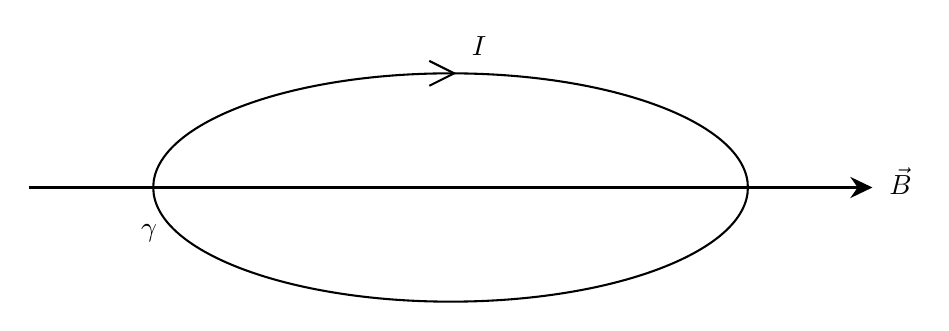
\begin{tikzpicture}[x=0.75pt,y=0.75pt,yscale=-1,xscale=1]
	%uncomment if require: \path (0,300); %set diagram left start at 0, and has height of 300

	%Shape: Ellipse [id:dp81007255868101] 
	\draw   (153,146) .. controls (153,115.62) and (217.14,91) .. (296.25,91) .. controls (375.36,91) and (439.5,115.62) .. (439.5,146) .. controls (439.5,176.38) and (375.36,201) .. (296.25,201) .. controls (217.14,201) and (153,176.38) .. (153,146) -- cycle ;
	\draw   (286,85) -- (298,91) -- (286,97) ;
	%Straight Lines [id:da5676795332498741] 
	\draw    (93,146) -- (496.5,146) ;
	\draw [shift={(499.5,146)}, rotate = 180] [fill={rgb, 255:red, 0; green, 0; blue, 0 }  ][line width=0.08]  [draw opacity=0] (10.72,-5.15) -- (0,0) -- (10.72,5.15) -- (7.12,0) -- cycle    ;

	% Text Node
	\draw (513,143) node    {$\vec{B}$};
	% Text Node
	\draw (310,78) node    {$I$};
	% Text Node
	\draw (151,168) node    {$\gamma $};

	\end{tikzpicture}
\end{figure}
\FloatBarrier

Il fatto che la forza sia nulla non significa che non ci sia alcuna interazione fra campo magnetico e circuito. \emph{Non c'è traslazione ma ci potrà essere rotazione}.

\section{Campo magnetico agente su una spira e momento magnetico}

Consideriamo una spira piana, rettangolare e rigida come in figura.

\begin{figure}[htpb]
	\centering

	\tikzset{every picture/.style={line width=0.75pt}} %set default line width to 0.75pt        

	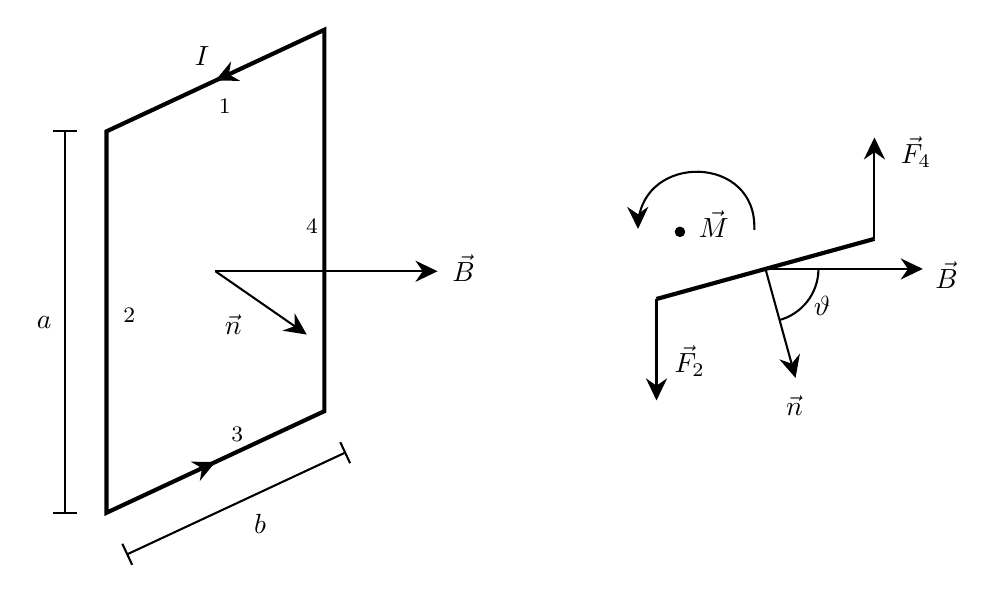
\begin{tikzpicture}[x=0.75pt,y=0.75pt,yscale=-1,xscale=1]
	%uncomment if require: \path (0,340); %set diagram left start at 0, and has height of 340

	%Shape: Rectangle [id:dp314599602769986] 
	\draw  [line width=1.5]  (243.5,23.64) -- (243.5,207.39) -- (138.5,256.36) -- (138.5,72.61) -- cycle ;
	%Straight Lines [id:da2971679923140418] 
	\draw    (118.5,72.61) -- (118.5,256.36) ;
	\draw [shift={(118.5,256.36)}, rotate = 270] [color={rgb, 255:red, 0; green, 0; blue, 0 }  ][line width=0.75]    (0,5.59) -- (0,-5.59)   ;
	\draw [shift={(118.5,72.61)}, rotate = 270] [color={rgb, 255:red, 0; green, 0; blue, 0 }  ][line width=0.75]    (0,5.59) -- (0,-5.59)   ;
	%Straight Lines [id:da3837571296766522] 
	\draw    (253.5,227.39) -- (148.5,276.36) ;
	\draw [shift={(148.5,276.36)}, rotate = 335] [color={rgb, 255:red, 0; green, 0; blue, 0 }  ][line width=0.75]    (0,5.59) -- (0,-5.59)   ;
	\draw [shift={(253.5,227.39)}, rotate = 335] [color={rgb, 255:red, 0; green, 0; blue, 0 }  ][line width=0.75]    (0,5.59) -- (0,-5.59)   ;
	%Straight Lines [id:da9220289196713451] 
	\draw    (191,140) -- (295,140) ;
	\draw [shift={(298,140)}, rotate = 180] [fill={rgb, 255:red, 0; green, 0; blue, 0 }  ][line width=0.08]  [draw opacity=0] (10.72,-5.15) -- (0,0) -- (10.72,5.15) -- (7.12,0) -- cycle    ;
	%Straight Lines [id:da49361292246796284] 
	\draw    (191,140) -- (232.53,168.79) ;
	\draw [shift={(235,170.5)}, rotate = 214.73] [fill={rgb, 255:red, 0; green, 0; blue, 0 }  ][line width=0.08]  [draw opacity=0] (10.72,-5.15) -- (0,0) -- (10.72,5.15) -- (7.12,0) -- cycle    ;
	%Straight Lines [id:da05198423899342308] 
	\draw    (243.5,23.64) -- (138.5,72.61) ;
	\draw [shift={(191,48.12)}, rotate = 335] [fill={rgb, 255:red, 0; green, 0; blue, 0 }  ][line width=0.08]  [draw opacity=0] (10.72,-5.15) -- (0,0) -- (10.72,5.15) -- (7.12,0) -- cycle    ;
	%Straight Lines [id:da5634924894683115] 
	\draw    (243.5,207.39) -- (138.5,256.36) ;
	\draw [shift={(191,231.88)}, rotate = 155] [fill={rgb, 255:red, 0; green, 0; blue, 0 }  ][line width=0.08]  [draw opacity=0] (10.72,-5.15) -- (0,0) -- (10.72,5.15) -- (7.12,0) -- cycle    ;
	%Straight Lines [id:da6157860000143798] 
	\draw [line width=1.5]    (403.5,153.36) -- (508.5,124.39) ;
	%Straight Lines [id:da5362688552515869] 
	\draw    (508.5,124.39) -- (508.5,78.5) ;
	\draw [shift={(508.5,75.5)}, rotate = 450] [fill={rgb, 255:red, 0; green, 0; blue, 0 }  ][line width=0.08]  [draw opacity=0] (10.72,-5.15) -- (0,0) -- (10.72,5.15) -- (7.12,0) -- cycle    ;
	%Straight Lines [id:da880907260663218] 
	\draw    (403.5,199.25) -- (403.5,153.36) ;
	\draw [shift={(403.5,202.25)}, rotate = 270] [fill={rgb, 255:red, 0; green, 0; blue, 0 }  ][line width=0.08]  [draw opacity=0] (10.72,-5.15) -- (0,0) -- (10.72,5.15) -- (7.12,0) -- cycle    ;
	%Straight Lines [id:da24430913160095735] 
	\draw    (456,138.88) -- (469.68,188.48) ;
	\draw [shift={(470.48,191.38)}, rotate = 254.57999999999998] [fill={rgb, 255:red, 0; green, 0; blue, 0 }  ][line width=0.08]  [draw opacity=0] (10.72,-5.15) -- (0,0) -- (10.72,5.15) -- (7.12,0) -- cycle    ;
	%Straight Lines [id:da5766759564623969] 
	\draw    (456,138.88) -- (528.8,138.88) ;
	\draw [shift={(531.8,138.88)}, rotate = 180] [fill={rgb, 255:red, 0; green, 0; blue, 0 }  ][line width=0.08]  [draw opacity=0] (10.72,-5.15) -- (0,0) -- (10.72,5.15) -- (7.12,0) -- cycle    ;
	%Shape: Arc [id:dp19135976738545968] 
	\draw  [draw opacity=0] (481.52,139.08) .. controls (481.43,150.8) and (473.44,160.64) .. (462.61,163.54) -- (456,138.88) -- cycle ; \draw   (481.52,139.08) .. controls (481.43,150.8) and (473.44,160.64) .. (462.61,163.54) ;
	%Curve Lines [id:da74730732313342] 
	\draw    (450.6,120) .. controls (452.16,83.73) and (397.06,82.82) .. (394.68,116.91) ;
	\draw [shift={(394.6,119.6)}, rotate = 269.38] [fill={rgb, 255:red, 0; green, 0; blue, 0 }  ][line width=0.08]  [draw opacity=0] (10.72,-5.15) -- (0,0) -- (10.72,5.15) -- (7.12,0) -- cycle    ;
	%Shape: Circle [id:dp7235812700074382] 
	\draw  [fill={rgb, 255:red, 0; green, 0; blue, 0 }  ,fill opacity=1 ] (412.8,121) .. controls (412.8,119.9) and (413.7,119) .. (414.8,119) .. controls (415.9,119) and (416.8,119.9) .. (416.8,121) .. controls (416.8,122.1) and (415.9,123) .. (414.8,123) .. controls (413.7,123) and (412.8,122.1) .. (412.8,121) -- cycle ;

	% Text Node
	\draw (108.5,164.48) node    {$a$};
	% Text Node
	\draw (212.5,261.52) node    {$b$};
	% Text Node
	\draw (310.5,138.48) node    {$\vec{B}$};
	% Text Node
	\draw (199.5,165.48) node    {$\vec{n}$};
	% Text Node
	\draw (195.5,60.48) node  [font=\footnotesize]  {$1$};
	% Text Node
	\draw (149.5,161.48) node  [font=\footnotesize]  {$2$};
	% Text Node
	\draw (201.5,218.48) node  [font=\footnotesize]  {$3$};
	% Text Node
	\draw (237.5,118.48) node  [font=\footnotesize]  {$4$};
	% Text Node
	\draw (184.5,36.48) node  [font=\normalsize]  {$I$};
	% Text Node
	\draw (528.5,82.48) node    {$\vec{F}_{4}$};
	% Text Node
	\draw (419.5,183.48) node    {$\vec{F}_{2}$};
	% Text Node
	\draw (469.9,204.68) node    {$\vec{n}$};
	% Text Node
	\draw (543.3,142.08) node    {$\vec{B}$};
	% Text Node
	\draw (483.3,156.88) node    {$\vartheta $};
	% Text Node
	\draw (431.1,117.48) node    {$\vec{M}$};

	\end{tikzpicture}
\end{figure}
\FloatBarrier

Assumiamo che ci sia una normale ortogonale al piano della spira e che essa si trovi in una regione in cui è presente un campo magnetico uniforme diretto in modo tale da essere perpendicolare ai lati maggiori di lunghezza $a$.
I fili percorsi da correnti sono sottoposti a forze magnetiche. Possiamo calcolare per ciascuno dei quattro lati l'andamento delle forze. Come si deduce dalla figura, le forze $\vec{F}_1$ ed $\vec{F}_3$ sono eguali e contrarie e hanno la stessa retta di azione. Nel loro insieme formano una coppia di braccio nullo e quindi un momento nullo. Per quanto riguarda $\vec{F}_4$ ed $\vec{F}_2$, anche tali forze hanno lo stesso modulo ma costituiscono una coppia di braccio $b\sin \vartheta$, dove $ \vartheta$ è l'angolo che $\vec{B}$ forma con la normale.

\begin{gather*}
	\vec{F} =I\vec{l} \times \vec{B} \qquad \vec{F}_3=-\vec{F}_1 \qquad \vec{F}_2 = -\vec{F}_4 \\
	\vec{R} = \vec{F}_1+\vec{F}_2+\vec{F}_3+\vec{F}_4
\end{gather*}

Calcoliamo il modulo della forza $ \vec{F}_4$ e il momento ad essa associato.

\[
	|\vec{F}_4 |=I\,a\,B \qquad |\vec{M} |=|\vec{F}_4 |\cdot \text{braccio} = I\,a\,B\,b\,\sin \vartheta = ISB\,\sin \vartheta
\]

Quindi

\[
	\vec{M} = IS\vec{n} \times \vec{B}
\]

Per analogia col campo elettrico si introduce il \emph{momento di dipolo magnetico della forza} come

\[
	\boxed{\vec{m} =IS\vec{n}} \implies \boxed{\vec{M} =\vec{m} \times \vec{B}}
\]

Questa formula ci dice che se consideriamo un magnete permanente immerso in un campo magnetico $\vec{B}$, anche su questo magnete agisce un campo delle forze che tende a farlo ruotare e quindi potremmo scrivere il momento delle forze agenti sul magente come abbiamo visto. Esso è una proprietà dell'ago magnetico che va misurata.

\begin{figure}[htpb]
	\centering

	\tikzset{every picture/.style={line width=0.75pt}} %set default line width to 0.75pt        

	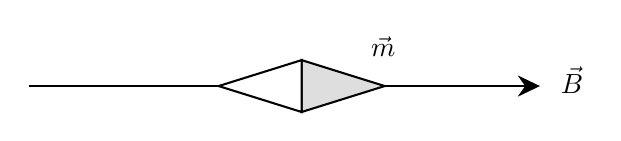
\begin{tikzpicture}[x=0.75pt,y=0.75pt,yscale=-1,xscale=1]
	%uncomment if require: \path (0,300); %set diagram left start at 0, and has height of 300

	%Straight Lines [id:da05135261111632694] 
	\draw    (82.5,135) -- (325.8,135) ;
	\draw [shift={(328.8,135)}, rotate = 180] [fill={rgb, 255:red, 0; green, 0; blue, 0 }  ][line width=0.08]  [draw opacity=0] (10.72,-5.15) -- (0,0) -- (10.72,5.15) -- (7.12,0) -- cycle    ;
	%Shape: Triangle [id:dp9590788161473491] 
	\draw  [fill={rgb, 255:red, 222; green, 222; blue, 222 }  ,fill opacity=1 ] (254,135) -- (214,147.5) -- (214,122.5) -- cycle ;
	%Shape: Triangle [id:dp8011408545698926] 
	\draw  [fill={rgb, 255:red, 255; green, 255; blue, 255 }  ,fill opacity=1 ] (174,135) -- (214,122.5) -- (214,147.5) -- cycle ;

	% Text Node
	\draw (344.3,132.08) node    {$\vec{B}$};
	% Text Node
	\draw (253.3,116.08) node    {$\vec{m}$};

	\end{tikzpicture}
\end{figure}
\FloatBarrier

Il risultato è valido in realtà per un circuito piano di forma qualunque immerso in un campo magnetico uniforme. Infatti il circuito si può sempre approssimare con n circuiti rettangolari adiacenti, tutti percorsi da una stessa corrente i con verso tale da avere le normali concordemente orientate. Le correnti che passano nei lati in comune sono eguali ed opposte per cui gli effetti del campo magnetico si annullano e rimangono solo gli effetti prodotti sul contorno esterno, coincidente con il circuito.

\begin{figure}[htpb]
	\centering

	\tikzset{every picture/.style={line width=0.75pt}} %set default line width to 0.75pt        

	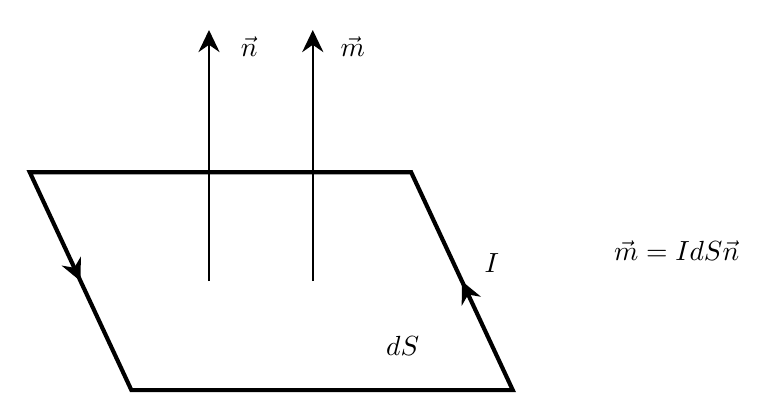
\begin{tikzpicture}[x=0.75pt,y=0.75pt,yscale=-1,xscale=1]
	%uncomment if require: \path (0,300); %set diagram left start at 0, and has height of 300

	%Shape: Rectangle [id:dp2081961356269224] 
	\draw  [line width=1.5]  (388.36,213.5) -- (204.61,213.5) -- (155.64,108.5) -- (339.39,108.5) -- cycle ;
	%Straight Lines [id:da47375466830675284] 
	\draw    (388.36,213.5) -- (339.39,108.5) ;
	\draw [shift={(363.88,161)}, rotate = 425] [fill={rgb, 255:red, 0; green, 0; blue, 0 }  ][line width=0.08]  [draw opacity=0] (10.72,-5.15) -- (0,0) -- (10.72,5.15) -- (7.12,0) -- cycle    ;
	%Straight Lines [id:da1877948623602992] 
	\draw    (204.61,213.5) -- (155.64,108.5) ;
	\draw [shift={(180.12,161)}, rotate = 245] [fill={rgb, 255:red, 0; green, 0; blue, 0 }  ][line width=0.08]  [draw opacity=0] (10.72,-5.15) -- (0,0) -- (10.72,5.15) -- (7.12,0) -- cycle    ;
	%Straight Lines [id:da5368840401436481] 
	\draw    (292,161) -- (292,43) ;
	\draw [shift={(292,40)}, rotate = 450] [fill={rgb, 255:red, 0; green, 0; blue, 0 }  ][line width=0.08]  [draw opacity=0] (10.72,-5.15) -- (0,0) -- (10.72,5.15) -- (7.12,0) -- cycle    ;
	%Straight Lines [id:da8370373990593616] 
	\draw    (242,161) -- (242,43) ;
	\draw [shift={(242,40)}, rotate = 450] [fill={rgb, 255:red, 0; green, 0; blue, 0 }  ][line width=0.08]  [draw opacity=0] (10.72,-5.15) -- (0,0) -- (10.72,5.15) -- (7.12,0) -- cycle    ;

	% Text Node
	\draw (311.3,48.08) node    {$\vec{m}$};
	% Text Node
	\draw (261.3,48.08) node    {$\vec{n}$};
	% Text Node
	\draw (467.3,146.08) node    {$\vec{m} =IdS\vec{n}$};
	% Text Node
	\draw (378.3,152.08) node    {$I$};
	% Text Node
	\draw (335.3,192.08) node    {$dS$};

	\end{tikzpicture}
\end{figure}
\FloatBarrier

Il momento risulta nullo soltanto se $\vec{m}$ è parallelo a $\vec{B}$. La posizione con $ \vartheta =0 $ è di equilibrio stabile, con $\vartheta =\pi$, di equilibrio instabile. Per qualsiasi altro angolo $\vec{M}$ tende a far ruotare la spira in modo che il momento magnetico $\vec{m}$ diventi parallelo a $\vec{B}$. Sospendendo opportunamente la spira è possibile generare in questo modo un moto oscillatorio. Ed è così che tramite l'orientazione di un piccolo circuito si possono ottenere direzione e verso di $\vec{B}$, mentre dalle piccole oscillazioni se ne deduce il modulo. Anche un ago magnetico ha un comportamento del tutto simile quando posto in un campo magnetico. Questa identità di comportamento fra quest'ultimo e la spira nei riguardi delle azioni meccaniche subite quando posti in un campo magnetico uniforme venne generalizzata da Ampere sottoforma di un postulato detto principio di equivalenza di Ampere. Afferma che una spira di area $ d\Sigma$ percorsa dalla corrente i equivale agli effetti magnetici a un dipolo elementare di momento magnetico perpendicolare al piano della spira e orientato rispetto al verso della corrente secondo la regola della vite. In analogia con quanto visto per il dipolo elettrico, anche per il dipolo magnetico si definisce un energia potenziale, legata alla posizione angolare rispetto alla direzione di $\vec{B}$. Si parla di energia potenziale magnetostatica ed è pari a:

\[
	\boxed{U_m = -\vec{m} \cdot \vec{B}}
\]

Questo deriva dal fatto che le interazioni tra il campo e il dipolo sono del tutto analoghe.

\section{Espressioni di forza, momento e lavoro tramite flusso magnetico}

Immaginiamo di considerare un circuito $\gamma$ di forma generica percorso da corrente $I$. Immaginiamo di costruire su questo circuito una superficie $\Sigma$ che abbia $\gamma$ come contorno o, come si dice, che si appoggi sul circuito $\gamma$. Possiamo pensare questo circuito come ricoperto da tante spire elementari percorse dalla stessa corrente $I$. Se prendiamo due spirette vicine, le correnti sui lati adiacenti si cancellano e rimangono solo le correnti sul bordo che rappresentano il circuito percorso da corrente. A questo punto possiamo immaginare che ci sia un campo magnetico e chiederci quanto valga l'energia magnetostatica. Dato che il circuito è equivalente alla scomposizione in tante spire, possiamo scrivere l'energia potenziale come la somma dell'energia potenziale di ciascuna di esse.

\[
	U_m=\int_{\Sigma}(-I\,dS\,\vec{n} ) \cdot \vec{B} = -I\int_{\Sigma}dS\,\vec{n} \cdot \vec{B} = -I\int_{\Sigma}\vec{B} \cdot \vec{n} \,dS
\]

L'ultimo integrale è il flusso di $\vec{B}$ concatenato al circuito.

\begin{figure}[htpb]
	\centering

	\tikzset{every picture/.style={line width=0.75pt}} %set default line width to 0.75pt        

	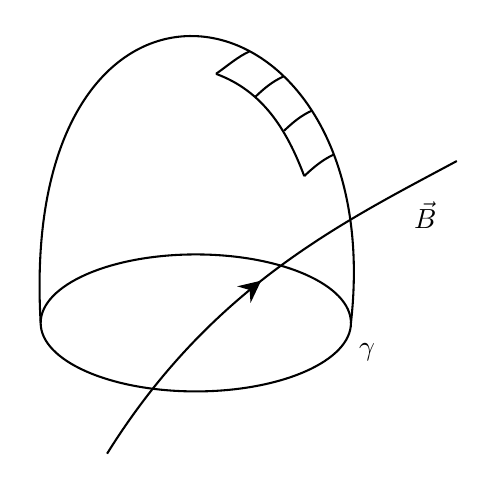
\begin{tikzpicture}[x=0.75pt,y=0.75pt,yscale=-1,xscale=1]
	%uncomment if require: \path (0,300); %set diagram left start at 0, and has height of 300

	%Shape: Ellipse [id:dp09744228681476397] 
	\draw   (201,200) .. controls (201,181.77) and (234.47,167) .. (275.75,167) .. controls (317.03,167) and (350.5,181.77) .. (350.5,200) .. controls (350.5,218.23) and (317.03,233) .. (275.75,233) .. controls (234.47,233) and (201,218.23) .. (201,200) -- cycle ;
	%Curve Lines [id:da7130016733280224] 
	\draw    (201,200) .. controls (195.25,100.5) and (237.38,58.25) .. (278.56,62) .. controls (319.75,65.75) and (360,115.5) .. (350.5,200) ;
	%Curve Lines [id:da7554171546591242] 
	\draw    (233,263) .. controls (283.5,182) and (347.5,151) .. (401.5,122) ;
	\draw [shift={(307.23,179.65)}, rotate = 501.13] [fill={rgb, 255:red, 0; green, 0; blue, 0 }  ][line width=0.08]  [draw opacity=0] (10.72,-5.15) -- (0,0) -- (10.72,5.15) -- (7.12,0) -- cycle    ;
	%Curve Lines [id:da41275262296503756] 
	\draw    (285.5,80) .. controls (308,88.25) and (319.5,106.75) .. (328,129.25) ;
	%Curve Lines [id:da020627173159082357] 
	\draw    (285.5,80) .. controls (291.5,75.75) and (296,71.75) .. (301.5,69.25) ;
	%Curve Lines [id:da8534082517799799] 
	\draw    (304.5,91) .. controls (308.6,87.1) and (312.5,83.75) .. (318,81.25) ;
	%Curve Lines [id:da5576041821757687] 
	\draw    (318.3,107.4) .. controls (322.4,103.5) and (326.3,100.15) .. (331.8,97.65) ;
	%Curve Lines [id:da2810794442426652] 
	\draw    (328,129.25) .. controls (332.1,125.35) and (336.7,121.4) .. (342.2,118.9) ;

	% Text Node
	\draw (386.3,148.08) node    {$\vec{B}$};
	% Text Node
	\draw (358.3,214.08) node    {$\gamma $};

	\end{tikzpicture}
\end{figure}
\FloatBarrier

Al circuito possiamo associare un energia magnetica pari a

\[
	\boxed{U_m=-I\cdot \Phi_{\Sigma}(\vec{B})}
\]

Il flusso di $\vec{B}$, essendo il campo solenoidale, non dipende dalla particolare superficie $\Sigma$ che si appoggia su $\gamma$. La formula per $U_m$ è determinata fissato il circuito e afferma che l'energia potenziale di un circuito percorso da corrente $I$ e immerso in un campo magnetico $\vec{B}$ è eguale al prodotto cambiato di segno della corrente per il flusso di $\vec{B}$ concatenato al circuito.
Il circuito può subire traslazione, deformazione o rotazione. A seguito di una di queste trasformazioni infinitesime il flusso del campo magnetico cambierà. Avremo una variazione dell'energia $dU$. Per calcolarla assumeremo che la corrente che scorre nel circuito rimanga la stessa (condizione essenziale per la validità delle seguenti formule). Notiamo che:

\begin{align*}
	dU_m=-I\,d\Phi \qquad d\mathcal{L} &=-dU_m=-(-I\,d\Phi )= I\,d\Phi\\
	\Aboxed{d\mathcal{L} &= I\,d\Phi}
\end{align*}

Possiamo allora riscrivere la risultante delle forze come

\begin{align*}
	\vec{R} &= - \vec{\nabla} U_m \\
	&= -\vec{\nabla} (-I\,\Phi (\vec{B} )) \\
	&= \vec{\nabla}(I\,\Phi (\vec{B} )) \\
	\Aboxed{\vec{R} &= \vec{\nabla}(I\,\Phi (\vec{B} ))}
\end{align*}

Questo risultato comunica che un circuito immerso in un campo magnetico variabile, è sottoposto a una risultante che punta nella direzione di massima crescita del flusso. Notiamo che si tratta di un risultato analogo a quello ottenuto per i bipoli elettrici sottoposti ad un campo $\vec{E}$, che sono portati ad allinearsi nella direzione di $\vec{E}$:

\[
	\vec{R} = - \vec{\nabla} U_e = -\vec{\nabla} (-p\vec{E} )
\]

\section{Campo magnetico prodotto da un circuito percorso da corrente (I legge di Laplace)}

Si dimostra che, considerato un tratto di circuito infinitesimo in cui scorre una corrente $I$, detto $dl$ il solito vettore spostamento parallelo al tratto di filo, considerato un punto $P$ dello spazio e introdotto un vettore $\vec{r}$ che punta al punto $P$, vale la legge:

\[
	\boxed{d\vec{B} (P)=\frac{\mu_0}{4\pi}\frac{I\,d\vec{l} \times \vec{u}_r}{r^2}}
\]

Nota come prima \textbf{legge di Laplace}.

\begin{figure}[htpb]
	\centering

	\tikzset{every picture/.style={line width=0.75pt}} %set default line width to 0.75pt        

	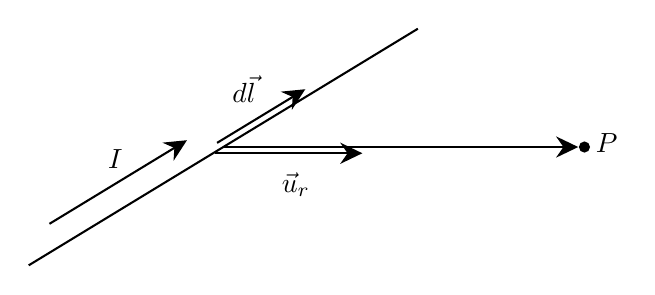
\begin{tikzpicture}[x=0.75pt,y=0.75pt,yscale=-1,xscale=1]
	%uncomment if require: \path (0,300); %set diagram left start at 0, and has height of 300

	%Straight Lines [id:da8727482290757451] 
	\draw    (352.75,96) -- (165.25,210) ;
	%Straight Lines [id:da8359628816789753] 
	\draw    (259,153) -- (427,153) ;
	\draw [shift={(430,153)}, rotate = 180] [fill={rgb, 255:red, 0; green, 0; blue, 0 }  ][line width=0.08]  [draw opacity=0] (10.72,-5.15) -- (0,0) -- (10.72,5.15) -- (7.12,0) -- cycle    ;
	%Straight Lines [id:da4970483138809967] 
	\draw    (238.94,151.28) -- (175.25,190) ;
	\draw [shift={(241.5,149.72)}, rotate = 148.7] [fill={rgb, 255:red, 0; green, 0; blue, 0 }  ][line width=0.08]  [draw opacity=0] (10.72,-5.15) -- (0,0) -- (10.72,5.15) -- (7.12,0) -- cycle    ;
	%Straight Lines [id:da159245909182834] 
	\draw    (295.94,126.72) -- (256,151) ;
	\draw [shift={(298.5,125.16)}, rotate = 148.7] [fill={rgb, 255:red, 0; green, 0; blue, 0 }  ][line width=0.08]  [draw opacity=0] (10.72,-5.15) -- (0,0) -- (10.72,5.15) -- (7.12,0) -- cycle    ;
	%Straight Lines [id:da43119170963545916] 
	\draw    (255,156) -- (323,156) ;
	\draw [shift={(326,156)}, rotate = 180] [fill={rgb, 255:red, 0; green, 0; blue, 0 }  ][line width=0.08]  [draw opacity=0] (10.72,-5.15) -- (0,0) -- (10.72,5.15) -- (7.12,0) -- cycle    ;
	%Shape: Circle [id:dp13708648389322597] 
	\draw  [fill={rgb, 255:red, 0; green, 0; blue, 0 }  ,fill opacity=1 ] (430.86,153) .. controls (430.86,151.82) and (431.82,150.86) .. (433,150.86) .. controls (434.18,150.86) and (435.14,151.82) .. (435.14,153) .. controls (435.14,154.18) and (434.18,155.14) .. (433,155.14) .. controls (431.82,155.14) and (430.86,154.18) .. (430.86,153) -- cycle ;

	% Text Node
	\draw (443.71,151.14) node    {$P$};
	% Text Node
	\draw (207,159) node    {$I$};
	% Text Node
	\draw (269,125) node    {$d\vec{l}$};
	% Text Node
	\draw (294,171) node    {$\vec{u}_{r}$};

	\end{tikzpicture}
\end{figure}
\FloatBarrier

Il campo magnetico elementare di un tratto infinitesimo di circuito risulta proporzionale alla corrente e inversamente proporzionale al quadrato della distanza. Tale formula ha validità generale, però soltanto come strumento matematico di calcolo; valgono infatti in proposito osservazioni analoghe a quelle fatte per la seconda legge elementare di Laplace: sperimentalmente non è possibile misurare in alcun modo il contributo di un elemento infinitesimo di filo, che a sua volta non può esistere da solo.
Per calcolare il campo magnetico di un circuito chiuso percorso da corrente si applica il principio di sovrapposizione degli effetti. Si scompone il circuito in tanti trattini infinitesimi, per ciascuno di essi si individua il vettore $\vec{r}$. Il campo complessivo sarà dato da

\[
	\vec{B} (P) = \int_{\gamma} \frac{\mu_0}{4\pi}\frac{I\,d\vec{l} \times \vec{r}}{r^3}
\]

Dove la costante vale $ \mu_0 = 4\pi \cdot 10^{-7} Tm/A $.

Per creare campi magnetici Intensi sono necessarie correnti molto elevate, visto il valore piccolo della costante.
Tale legge si può applicare anche nel caso di conduttori macroscopici immaginandoli come un fascio di fili percorsi da corrente. Infatti si considera un elemento di sezione $dS$ percorso da corrente di densità $\vec{J}(x,y,z)$. Allora si ha:

\begin{gather*}
	di=J\,dS \implies d\vec{B} (P)=\frac{\mu_0}{4\pi}\frac{I\,d\vec{l} \times \vec{r}}{r^3} = \frac{\mu_0}{4\pi} \frac{\vec{J} \times \vec{r} \,\overbrace{dS\,dl}^{d\tau}}{r^3} \\
	\boxed{\vec{B} (P)= \int_{\gamma}\frac{\mu_0}{4\pi}\frac{\vec{J} \times \vec{r}}{r^3}d\tau}
\end{gather*}

\section{Campo magnetico prodotto da una carica in moto}

Avevamo introdotto una formula approssimata per il campo elettrico generato da un dipolo, che può essere scritto come

\[
	\vec{E} (P)= \frac{3(\vec{p} \cdot \vec{u}_r)\vec{u}_r-\vec{p}}{4\pi r^3}
\]

Nel caso del magnete, considerato un punto alla distanza $P$, detta $r$ la distanza fra l'oggetto e il punto $P$, avremo che il campo magnetico avrà una formula analoga

\[
	\vec{B} (P)=\frac{\mu_0}{4\pi}\frac{3(\vec{m} \cdot \vec{u}_r)\vec{u}_r-\vec{m}}{r^3}
\]

Se in un conduttore di corrente $\vec{J}$ consideriamo un tratto infinitesimo, possiamo calcolare il contributo al campo magnetico di questa porzione di conduttore utilizzando le solite formule. Il contributo al campo magnetico nel punto $P$ era:

\[
	d\vec{B} (P)= \frac{\mu_0}{4\pi}\frac{\vec{J} \times \vec{r}}{r^3}d\tau =\frac{\mu_0}{4\pi}\frac{\vec{J} \times \vec{u}_r}{r^2}d\tau
\]

Ricordiamo che la densità di corrente è legata alla velocità dei portatori di carica e al loro numero per unità di volume da:

\begin{gather*}
	\vec{J} =n\,q\,\vec{v}_d \qquad d\tau \cdot n=N \\
	d\vec{B} (P)= \frac{\mu_0}{4\pi}\frac{q\,n\,\vec{v}_d\times \vec{u}_r}{r^2}d\tau = \frac{\mu_0}{4\pi}\frac{q\,\vec{v}_d\times \vec{u}_r}{r^2}dN
\end{gather*}

Guardando la formula di questo modo, osserviamo che il campo magnetico è il prodotto di qualcosa per il numero di cariche presenti nell'elementino. Se dividiamo per il numero di cariche otteniamo il campo magnetico prodotto dalla singola carica.

\[
	\frac{d\vec{B}}{dN}=\frac{\mu_0}{4\pi}\frac{q\,\vec{v}_d\times \vec{u}_r}{r^2} = \vec{B}_{\text{singola carica}}
\]

Una carica elettrica in moto o in quiete genera anche un campo elettrico. Nel punto $P$ oltre al campo magnetico ci sarà anche un campo elettrico:

\[
	\vec{E} (P)_{\text{singola carica}} = \frac{q}{4\pi \varepsilon_0} \vec{u}_r
\]

Possiamo cercare una connessione fra le due formule. Possiamo vedere il campo magnetico come:

\[
	\vec{B} (P)_{\text{sc}} = \frac{\vec{v}_d\times q\vec{u}_r}{4\pi r^2 \varepsilon_0} \varepsilon_0 \mu_0  \implies  \vec{B} (P) = \mu_0 \varepsilon_0 \,\vec{v} \times \vec{E} (P) \qquad \mu_0 \varepsilon_0 = \frac{1}{c^2}
\]

Stabilendo una stretta relazione tra campo elettrico e magnetico prodotti da una carica in moto, essendo c la velocità della luce nel vuoto. La formula trovata per il campo magnetico prodotto dalla singola carica vale finché la velocità $v$ è trascurabile rispetto a, ossia finché $ (v/c)^2 \ll 1 $. Anche l'espressione del campo elettrico ha le stesse limitazioni.

\section{Legge di Biot-Savart (campo magnetico prodotto da un filo rettilineo infinito)}

Un sistema di riferimento è dato da:

\begin{itemize}
	\item $\vec{u}_n$ versore perpendicolare al filo, diretto verso $P$
	\item $\vec{u}_{\varphi}$ versore perpendicolare al piano del foglio con verso scelto con la regola della vite destrorsa (regola della mano destra)
	\item $\vec{u}_t$ versore tangente al filo
\end{itemize}

\[
	\implies \vec{u}_{\varphi}=\vec{u}_t\times \vec{u}_n
\]

\begin{figure}[htpb]
	\centering

	\tikzset{every picture/.style={line width=0.75pt}} %set default line width to 0.75pt        

	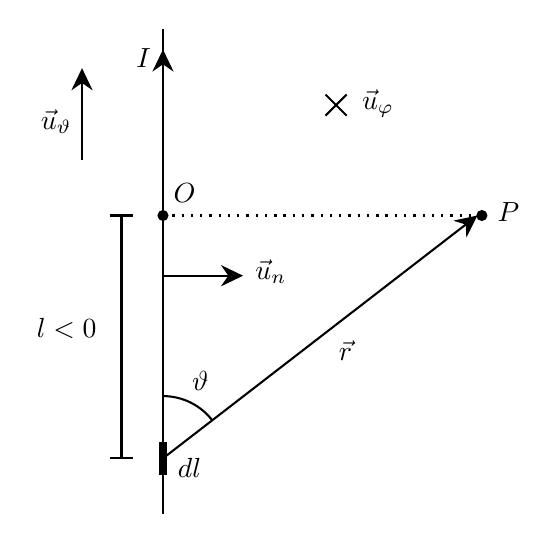
\begin{tikzpicture}[x=0.75pt,y=0.75pt,yscale=-1,xscale=1]
	%uncomment if require: \path (0,300); %set diagram left start at 0, and has height of 300

	%Straight Lines [id:da400490808663277] 
	\draw    (200,29) -- (200,263) ;
	%Straight Lines [id:da45879608678252115] 
	\draw    (200,83.4) -- (200,42) ;
	\draw [shift={(200,39)}, rotate = 450] [fill={rgb, 255:red, 0; green, 0; blue, 0 }  ][line width=0.08]  [draw opacity=0] (10.72,-5.15) -- (0,0) -- (10.72,5.15) -- (7.12,0) -- cycle    ;
	%Straight Lines [id:da4761857626496162] 
	\draw  [dash pattern={on 0.84pt off 2.51pt}]  (200,119) -- (351.5,119) ;
	%Straight Lines [id:da24289172597636122] 
	\draw    (200,236) -- (349.13,120.83) ;
	\draw [shift={(351.5,119)}, rotate = 502.32] [fill={rgb, 255:red, 0; green, 0; blue, 0 }  ][line width=0.08]  [draw opacity=0] (10.72,-5.15) -- (0,0) -- (10.72,5.15) -- (7.12,0) -- cycle    ;
	%Shape: Circle [id:dp6692413966506952] 
	\draw  [fill={rgb, 255:red, 0; green, 0; blue, 0 }  ,fill opacity=1 ] (351.5,119) .. controls (351.5,117.82) and (352.46,116.86) .. (353.64,116.86) .. controls (354.83,116.86) and (355.79,117.82) .. (355.79,119) .. controls (355.79,120.18) and (354.83,121.14) .. (353.64,121.14) .. controls (352.46,121.14) and (351.5,120.18) .. (351.5,119) -- cycle ;
	%Straight Lines [id:da9483799877637442] 
	\draw    (200,148) -- (235.6,148) ;
	\draw [shift={(238.6,148)}, rotate = 180] [fill={rgb, 255:red, 0; green, 0; blue, 0 }  ][line width=0.08]  [draw opacity=0] (10.72,-5.15) -- (0,0) -- (10.72,5.15) -- (7.12,0) -- cycle    ;
	%Shape: Rectangle [id:dp2511783145268558] 
	\draw  [fill={rgb, 255:red, 0; green, 0; blue, 0 }  ,fill opacity=1 ] (198.6,228.4) -- (201.4,228.4) -- (201.4,243.6) -- (198.6,243.6) -- cycle ;
	%Shape: Arc [id:dp06720596056852024] 
	\draw  [draw opacity=0] (199.91,206) .. controls (199.94,206) and (199.97,206) .. (200,206) .. controls (209.65,206) and (218.23,210.56) .. (223.72,217.63) -- (200,236) -- cycle ; \draw   (199.91,206) .. controls (199.94,206) and (199.97,206) .. (200,206) .. controls (209.65,206) and (218.23,210.56) .. (223.72,217.63) ;
	%Straight Lines [id:da6085603141380644] 
	\draw    (180,236) -- (180,119) ;
	\draw [shift={(180,119)}, rotate = 450] [color={rgb, 255:red, 0; green, 0; blue, 0 }  ][line width=0.75]    (0,5.59) -- (0,-5.59)   ;
	\draw [shift={(180,236)}, rotate = 450] [color={rgb, 255:red, 0; green, 0; blue, 0 }  ][line width=0.75]    (0,5.59) -- (0,-5.59)   ;
	%Shape: Circle [id:dp6334725741706344] 
	\draw  [fill={rgb, 255:red, 0; green, 0; blue, 0 }  ,fill opacity=1 ] (197.86,119) .. controls (197.86,117.82) and (198.82,116.86) .. (200,116.86) .. controls (201.18,116.86) and (202.14,117.82) .. (202.14,119) .. controls (202.14,120.18) and (201.18,121.14) .. (200,121.14) .. controls (198.82,121.14) and (197.86,120.18) .. (197.86,119) -- cycle ;
	\draw   (278.3,60.7) -- (288.5,70.9)(288.5,60.7) -- (278.3,70.9) ;
	%Straight Lines [id:da5318167544382137] 
	\draw    (161,92.4) -- (161,51) ;
	\draw [shift={(161,48)}, rotate = 450] [fill={rgb, 255:red, 0; green, 0; blue, 0 }  ][line width=0.08]  [draw opacity=0] (10.72,-5.15) -- (0,0) -- (10.72,5.15) -- (7.12,0) -- cycle    ;

	% Text Node
	\draw (190.6,43.2) node    {$I$};
	% Text Node
	\draw (288,184) node    {$\vec{r}$};
	% Text Node
	\draw (366.4,117.2) node    {$P$};
	% Text Node
	\draw (252,146) node    {$\vec{u}_{n}$};
	% Text Node
	\draw (218,198.8) node    {$\vartheta $};
	% Text Node
	\draw (210.4,108.4) node    {$O$};
	% Text Node
	\draw (153.6,173.6) node    {$l< 0$};
	% Text Node
	\draw (212.8,240.4) node    {$dl$};
	% Text Node
	\draw (303.6,65.2) node    {$\vec{u}_{\varphi }$};
	% Text Node
	\draw (148.6,73.8) node    {$\vec{u}_{\vartheta }$};

	\end{tikzpicture}
\end{figure}
\FloatBarrier

Applichiamo la legge di Laplace

\begin{gather*}
	d\vec{B} (P)=\frac{\mu_0}{4\pi}\frac{I\,d\vec{l} \times \vec{r}}{r^3} = \frac{\mu_0}{4\pi}\frac{I\,dl\,\sin \vartheta}{r^2}\vec{u}_{\varphi} \\
	\vec{B} (P)= \int_{\text{filo}}d\vec{B} (P) = \int_{\text{filo}} \frac{\mu_0}{4\pi}\frac{I\,dl\,\sin \vartheta}{r^2}\vec{u}_{\varphi}
\end{gather*}

Iniziamo a calcolare le solite relazioni per esprimere tutto in funzione degli angoli.

\begin{gather*}
	R=r\,\sin \vartheta \implies r=\frac{R}{\sin \vartheta} \qquad l= r\,\cos \vartheta = -R\,\text{cotan} \vartheta
\end{gather*}

Esprimiamo $ dl $ come

\begin{gather*}
	dl=\frac{dl}{d\vartheta}d\vartheta =\frac{d}{d\vartheta}(-R\,\text{cotan}\vartheta  )d\vartheta = -\left( -\frac{R}{\sin^2 \vartheta} \right) d\vartheta = \frac{R}{\sin^2 \vartheta} d\vartheta \\
	d\vec{B} (P)= \frac{\mu_0}{4\pi}\frac{I\, \overbrace{\frac{R}{\sin^2 \vartheta}d\vartheta}^{dl} \sin \vartheta}{\underbrace{\frac{R^2}{\sin^2 \vartheta}}_{r^2}}\vec{u}_{\varphi} = \frac{\mu_0}{4\pi}\frac{I\,\sin \vartheta}{R}\vec{u}_{\varphi}d\vartheta
\end{gather*}

Possiamo ora procedere con l'integrazione finale tra gli estremi dell'angolo

\begin{equation*}
	\begin{aligned}
		\vec{B} (P)= \int_0^{\pi} \frac{\mu_0 \,I\,\sin \vartheta}{4\pi R}\vec{u}_{\varphi}d\vartheta &= \frac{\mu_0 \,I\,\vec{u}_{\varphi}}{4\pi R}\int_0^{\pi} \sin \vartheta d\vartheta \\
		&= \frac{\mu_0 \,I\,\vec{u}_{\varphi}}{4\pi R} \underbrace{[-\cos \vartheta ]_0^{\pi}}_2 = \frac{\mu_0 I}{2\pi R}\vec{u}_{\varphi}
	\end{aligned}
\end{equation*}

Nel piano mediano il campo magnetico $\vec{B}$ è costante su ogni circonferenza di raggio $R$ ed è tangente a tale circonferenza. Detto $ \vec{u}_{\varphi} $ il versore tangente alla circonferenza e orientato rispetto al verso della corrente secondo la regola della vite, possiamo scrivere:

\[
	\vec{B} (P)=\frac{\mu_0 I}{2\pi R}\vec{u}_{\varphi}
\]

Tale risultato è noto come \textbf{legge di Biot-Savart} e afferma che il campo magnetico di un filo rettilineo indefinito dipende solo dalla distanza dal filo, in modo inversamente proporzionale, le sue linee sono circonferenze concentriche al filo.

\section{Interazione tra circuiti percorsi da corrente}

Calcoliamo ora la forza tra circuiti percorsi da corrente, partendo dalle leggi elementari di Laplace. Scomponiamo entrambi i circuiti in tanti elementi. Chiamiamo $r$ la distanza fra due elementi generici $dl_1$ e $dl_2$ e individuiamo con $\vec{u}_1$ il versore che punta da $dl_1$ a $dl_2$ e $\vec{u}_2$ il versore che punta in verso opposto.

\begin{figure}[htpb]
	\centering

	\tikzset{every picture/.style={line width=0.75pt}} %set default line width to 0.75pt        

	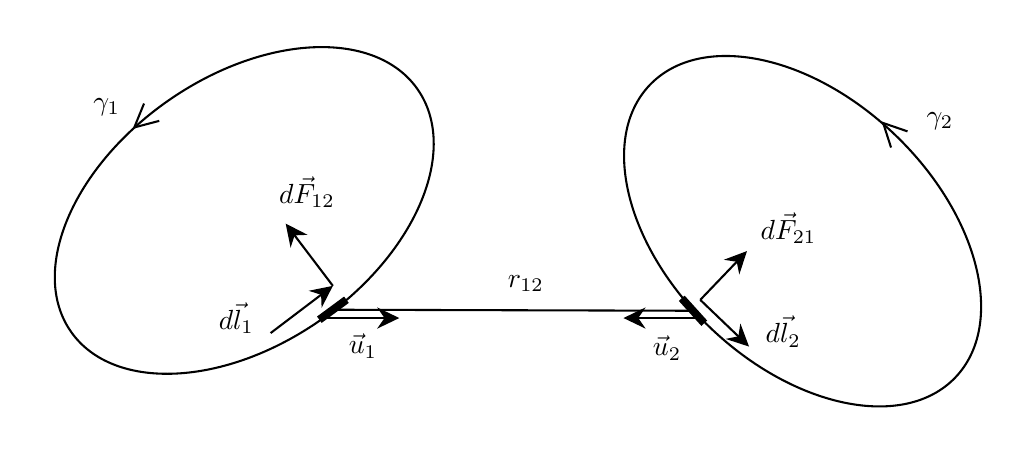
\begin{tikzpicture}[x=0.75pt,y=0.75pt,yscale=-1,xscale=1]
	%uncomment if require: \path (0,300); %set diagram left start at 0, and has height of 300

	%Shape: Ellipse [id:dp5039867707891208] 
	\draw   (85.33,188.11) .. controls (64.95,159) and (85.8,109.24) .. (131.89,76.96) .. controls (177.99,44.68) and (231.88,42.11) .. (252.26,71.22) .. controls (272.65,100.33) and (251.8,150.1) .. (205.71,182.37) .. controls (159.61,214.65) and (105.72,217.22) .. (85.33,188.11) -- cycle ;
	%Shape: Ellipse [id:dp4465357244059345] 
	\draw   (511.39,210.14) .. controls (486.81,235.81) and (433.94,225.06) .. (393.3,186.14) .. controls (352.65,147.22) and (339.63,94.86) .. (364.21,69.19) .. controls (388.79,43.53) and (441.66,54.27) .. (482.3,93.19) .. controls (522.95,132.11) and (535.97,184.47) .. (511.39,210.14) -- cycle ;
	%Shape: Rectangle [id:dp4793662673196728] 
	\draw  [fill={rgb, 255:red, 0; green, 0; blue, 0 }  ,fill opacity=1 ] (216.79,171.86) -- (218.45,174.12) -- (206.21,183.14) -- (204.55,180.88) -- cycle ;
	%Straight Lines [id:da36718365960822563] 
	\draw    (211.5,177.5) -- (385,178) ;
	\draw   (127.85,86.51) -- (115.82,89.67) -- (120.51,78.15) ;
	\draw   (480.42,99.36) -- (476.61,87.53) -- (488.36,91.58) ;
	%Shape: Rectangle [id:dp7299100063793511] 
	\draw  [fill={rgb, 255:red, 0; green, 0; blue, 0 }  ,fill opacity=1 ] (378.87,173.3) -- (380.94,171.42) -- (391.13,182.7) -- (389.06,184.58) -- cycle ;
	%Straight Lines [id:da6851940673219525] 
	\draw    (208.5,181.5) -- (240.5,181.5) ;
	\draw [shift={(243.5,181.5)}, rotate = 180] [fill={rgb, 255:red, 0; green, 0; blue, 0 }  ][line width=0.08]  [draw opacity=0] (10.72,-5.15) -- (0,0) -- (10.72,5.15) -- (7.12,0) -- cycle    ;
	%Straight Lines [id:da6416264107401324] 
	\draw    (354.5,181.5) -- (386.5,181.5) ;
	\draw [shift={(351.5,181.5)}, rotate = 0] [fill={rgb, 255:red, 0; green, 0; blue, 0 }  ][line width=0.08]  [draw opacity=0] (10.72,-5.15) -- (0,0) -- (10.72,5.15) -- (7.12,0) -- cycle    ;
	%Straight Lines [id:da46776015006269556] 
	\draw    (181.5,188.75) -- (209.11,167.81) ;
	\draw [shift={(211.5,166)}, rotate = 502.83] [fill={rgb, 255:red, 0; green, 0; blue, 0 }  ][line width=0.08]  [draw opacity=0] (10.72,-5.15) -- (0,0) -- (10.72,5.15) -- (7.12,0) -- cycle    ;
	%Straight Lines [id:da29499082211518535] 
	\draw    (211.5,166) -- (190.56,138.39) ;
	\draw [shift={(188.75,136)}, rotate = 412.83000000000004] [fill={rgb, 255:red, 0; green, 0; blue, 0 }  ][line width=0.08]  [draw opacity=0] (10.72,-5.15) -- (0,0) -- (10.72,5.15) -- (7.12,0) -- cycle    ;
	%Straight Lines [id:da5556095860689843] 
	\draw    (409.83,193.18) -- (388.5,172.75) ;
	\draw [shift={(412,195.25)}, rotate = 223.75] [fill={rgb, 255:red, 0; green, 0; blue, 0 }  ][line width=0.08]  [draw opacity=0] (10.72,-5.15) -- (0,0) -- (10.72,5.15) -- (7.12,0) -- cycle    ;
	%Straight Lines [id:da48897677161774156] 
	\draw    (388.5,172.75) -- (408.93,151.42) ;
	\draw [shift={(411,149.25)}, rotate = 493.75] [fill={rgb, 255:red, 0; green, 0; blue, 0 }  ][line width=0.08]  [draw opacity=0] (10.72,-5.15) -- (0,0) -- (10.72,5.15) -- (7.12,0) -- cycle    ;

	% Text Node
	\draw (304.5,165) node    {$r_{12}$};
	% Text Node
	\draw (226,195) node    {$\vec{u}_{1}$};
	% Text Node
	\draw (504,86.5) node    {$\gamma _{2}$};
	% Text Node
	\draw (102.5,80) node    {$\gamma _{1}$};
	% Text Node
	\draw (372.5,196) node    {$\vec{u}_{2}$};
	% Text Node
	\draw (165,181.5) node    {$d\vec{l}_{1}$};
	% Text Node
	\draw (199,121) node    {$d\vec{F}_{12}$};
	% Text Node
	\draw (428.5,188) node    {$d\vec{l}_{2}$};
	% Text Node
	\draw (431,138) node    {$d\vec{F}_{21}$};

	\end{tikzpicture}
\end{figure}
\FloatBarrier

Utilizzando la seconda legge di Laplace, sappiamo che la forza $d\vec{F}_{21}$ agente sull'elemento $dl_2$ a causa del campo magnetico $d\vec{B}_1$ prodotto da $dl_1$ nel posto in cui si trova $dl_2$ è

\[
	d\vec{F}_{21}=I_2d\vec{l}_2\times d\vec{B}_1
\]

Per la prima legge di Laplace si ha:

\begin{gather*}
	d\vec{B}_1=\frac{\mu_0}{4\pi}\frac{I_1d\vec{l}_1\times \vec{u}_1}{r^2} \\
	d\vec{F}_{21} = I_2d\vec{l}_2\times \left[ \frac{\mu_0}{4\pi}\frac{I_1d\vec{l}_1\times \vec{u}_1}{r^2}  \right] =\frac{\mu_0 I_1I_2}{4\pi r^2}d\vec{l}_2\times (d\vec{l}_1\times \vec{u}_1) \\
	d\vec{F}_{12} = I_1d\vec{l}_1\times \left[ \frac{\mu_0}{4\pi}\frac{I_2d\vec{l}_2\times \vec{u}_2}{r^2}  \right] = \frac{\mu_0 I_1I_2}{4\pi r^2}d\vec{l}_1\times (d\vec{l}_2\times \vec{u}_2 )
\end{gather*}

Quindi $ d\vec{F}_{21} \neq d\vec{F}_{12}$. Sembra che esse non rispettino il terzo principio della dinamica. Ma le due formule di Laplace non vanno prese come formule che rappresentano interazioni di tipo fondamentale, vanno prese come ausili matematici e integrate su tutto il circuito. A noi interessano per il principio azione reazione le forze totali. Le leggi elementari di Laplace infatti non si applicano a sistemi fisicamente realizzabili.

La forza risultante fra i due circuiti si ottiene con una doppia integrazione estesa ai due circuiti che tiene conto di tutte le coppie di elementi $dl_1$ e $dl_2$ tra i quali si esercitano le forze $d\vec{F}$:

\begin{align*}
	\left.\begin{array}{ll}
		\vec{F}_{21} = \oint_{c1} \oint_{c2} d\vec{F}_{21} \\
		\vec{F}_{12} = \oint_{c2} \oint_{c1} d\vec{F}_{12}
	\end{array}\right\}
		\implies \vec{F}_{21} = \vec{F}_{12}
\end{align*}

Si può verificare che la forza tra i due circuiti obbedisce al principio di azione reazione.

\section{Coefficiente di mutua e auto-induzione}

Il campo magnetico $B_1$ generato da un circuito percorso dalla corrente i1 determina un certo flusso magnetico attraverso un qualsiasi altro circuito presente nella regione in cui agisce $B_1$.

\begin{figure}[htpb]
	\centering

	% Pattern Info
	 
	\tikzset{
	pattern size/.store in=\mcSize, 
	pattern size = 5pt,
	pattern thickness/.store in=\mcThickness, 
	pattern thickness = 0.3pt,
	pattern radius/.store in=\mcRadius, 
	pattern radius = 1pt}
	\makeatletter
	\pgfutil@ifundefined{pgf@pattern@name@_x03l2yg0j}{
	\pgfdeclarepatternformonly[\mcThickness,\mcSize]{_x03l2yg0j}
	{\pgfqpoint{0pt}{0pt}}
	{\pgfpoint{\mcSize+\mcThickness}{\mcSize+\mcThickness}}
	{\pgfpoint{\mcSize}{\mcSize}}
	{
	\pgfsetcolor{\tikz@pattern@color}
	\pgfsetlinewidth{\mcThickness}
	\pgfpathmoveto{\pgfqpoint{0pt}{0pt}}
	\pgfpathlineto{\pgfpoint{\mcSize+\mcThickness}{\mcSize+\mcThickness}}
	\pgfusepath{stroke}
	}}
	\makeatother

	% Pattern Info
	 
	\tikzset{
	pattern size/.store in=\mcSize, 
	pattern size = 5pt,
	pattern thickness/.store in=\mcThickness, 
	pattern thickness = 0.3pt,
	pattern radius/.store in=\mcRadius, 
	pattern radius = 1pt}
	\makeatletter
	\pgfutil@ifundefined{pgf@pattern@name@_191ys6rbz}{
	\pgfdeclarepatternformonly[\mcThickness,\mcSize]{_191ys6rbz}
	{\pgfqpoint{0pt}{0pt}}
	{\pgfpoint{\mcSize+\mcThickness}{\mcSize+\mcThickness}}
	{\pgfpoint{\mcSize}{\mcSize}}
	{
	\pgfsetcolor{\tikz@pattern@color}
	\pgfsetlinewidth{\mcThickness}
	\pgfpathmoveto{\pgfqpoint{0pt}{0pt}}
	\pgfpathlineto{\pgfpoint{\mcSize+\mcThickness}{\mcSize+\mcThickness}}
	\pgfusepath{stroke}
	}}
	\makeatother
	\tikzset{every picture/.style={line width=0.75pt}} %set default line width to 0.75pt        

	\begin{tikzpicture}[x=0.75pt,y=0.75pt,yscale=-1,xscale=1]
	%uncomment if require: \path (0,300); %set diagram left start at 0, and has height of 300

	%Shape: Ellipse [id:dp5421393934180025] 
	\draw  [pattern=_x03l2yg0j,pattern size=6pt,pattern thickness=0.75pt,pattern radius=0pt, pattern color={rgb, 255:red, 222; green, 222; blue, 222}] (400.48,243.91) .. controls (371.1,223.92) and (372.94,170) .. (404.6,123.47) .. controls (436.25,76.94) and (485.73,55.43) .. (515.12,75.42) .. controls (544.5,95.41) and (542.65,149.34) .. (511,195.86) .. controls (479.34,242.39) and (429.86,263.9) .. (400.48,243.91) -- cycle ;
	%Shape: Ellipse [id:dp4806549724492446] 
	\draw  [pattern=_191ys6rbz,pattern size=6pt,pattern thickness=0.75pt,pattern radius=0pt, pattern color={rgb, 255:red, 222; green, 222; blue, 222}] (105.33,208.11) .. controls (84.95,179) and (105.8,129.24) .. (151.89,96.96) .. controls (197.99,64.68) and (251.88,62.11) .. (272.26,91.22) .. controls (292.65,120.33) and (271.8,170.1) .. (225.71,202.37) .. controls (179.61,234.65) and (125.72,237.22) .. (105.33,208.11) -- cycle ;
	\draw   (147.85,106.51) -- (135.82,109.67) -- (140.51,98.15) ;
	\draw   (504.6,195.03) -- (515.64,189.31) -- (513.6,201.57) ;
	%Straight Lines [id:da3399806485135666] 
	\draw    (457.8,159.67) -- (369.48,99.58) ;
	\draw [shift={(367,97.89)}, rotate = 394.23] [fill={rgb, 255:red, 0; green, 0; blue, 0 }  ][line width=0.08]  [draw opacity=0] (10.72,-5.15) -- (0,0) -- (10.72,5.15) -- (7.12,0) -- cycle    ;
	%Straight Lines [id:da06607489606794448] 
	\draw    (188.8,149.67) -- (126.72,61.01) ;
	\draw [shift={(125,58.55)}, rotate = 415] [fill={rgb, 255:red, 0; green, 0; blue, 0 }  ][line width=0.08]  [draw opacity=0] (10.72,-5.15) -- (0,0) -- (10.72,5.15) -- (7.12,0) -- cycle    ;

	% Text Node
	\draw (112,52) node    {$\vec{n}_{1}$};
	% Text Node
	\draw (551,161.5) node    {$\gamma _{2}$};
	% Text Node
	\draw (84.5,175) node    {$\gamma _{1}$};
	% Text Node
	\draw (230,219.5) node    {$d\vec{l}_{1}$};
	% Text Node
	\draw (374.5,236) node    {$d\vec{l}_{2}$};
	% Text Node
	\draw (354,92) node    {$\vec{n}_{2}$};
	% Text Node
	\draw (249,98.5) node    {$\Sigma _{1}$};
	% Text Node
	\draw (496,89.5) node    {$\Sigma _{2}$};
	% Text Node
	\draw (108.5,118) node    {$I_{1}$};
	% Text Node
	\draw (517.5,217) node    {$I_{2}$};

	\end{tikzpicture}
\end{figure}
\FloatBarrier

Si ottiene

\begin{gather*}
	\vec{B}_1(P)= \oint_{\gamma_1} \frac{\mu_0}{4\pi}\frac{I_1d\vec{l}_1\times \vec{u}_r}{r^2} \\
\end{gather*}

Calcoliamo il flusso di questo campo concatenato a un'altro circuito.

\begin{equation*}
	\begin{aligned}
		\Phi_{\Sigma_2}=\int_{\Sigma_2} \vec{B}_1(P)\cdot \vec{n}_2\,dS &= \int_{\Sigma_2} \left[ \oint_{\gamma_1} \frac{\mu_0}{4\pi}\frac{I_1d\vec{l}_1\times \vec{u}_r}{r^2} \right] \cdot \vec{n}_2 \,dS \\
		&= I_1 \underbrace{\int_{\Sigma_2} \left[ \oint_{\gamma_1} \frac{\mu_0}{4\pi}\frac{d\vec{l}_1\times \vec{u}_r}{r^2} \right] \cdot \vec{n}_2 \,dS}_{M_{21}}  = I_1\,M_{21}
	\end{aligned}
\end{equation*}

Dove $\Sigma_2$ è una qualsiasi superficie che si appoggia sul secondo circuito, $r$ è la distanza dall'elemento $d\vec{l}_1$ del primo circuito all'elemento di area $dS$ e $\vec{u}_r$ è il versore della direzione orientata $r$.
L'espressione del flusso può essere riscritta sinteticamente come:

\[
	\Phi_{21}=M_{21}I_1 \qquad \Phi_{12}=M_{12}I_2
\]

Conglobando in $M_{12}$ tutti i fattori geometrici e l'eventuale dipendenza dalle proprietà magnetiche del mezzo in cui sono immersi i circuiti (vale lo stesso discorso per il circuito $2$ rispetto all'$1$). Mi dice quanto vale il flusso attraverso il circuito $2$ a causa del campo prodotto dal circuito $1$ e prende il nome di \textbf{coefficiente di mutua induzione}. Si può dimostrare che i due coefficienti $M_{12}$ e $M_{21}$ sono uguali.

\[
	M_{21}=M_{12}
\]

Il campo magnetico generato da un circuito produce un flusso anche attraverso il circuito stesso, detto \textbf{autoflusso del circuito}, che si scrive:

\begin{gather*}
	\vec{B} = \oint_{\gamma} \frac{\mu_0}{4\pi}\frac{I\,d\vec{l} \times \vec{u}_r}{r^2}
\end{gather*}

\begin{equation*}
	\begin{aligned}
		\Phi_{\Sigma}(\vec{B} ) = \int_{\Sigma}\vec{B} \cdot \vec{n} \,dS &= \int_{\Sigma} \left[ \oint_{\gamma} \frac{\mu_0}{4\pi}\frac{I\,d\vec{l} \times \vec{u}_r}{r^2} \right]   \cdot \vec{n} \,dS \\
		&= I \underbrace{\int_{\Sigma} \left[ \oint_{\gamma} \frac{\mu_0}{4\pi}\frac{d\vec{l} \times \vec{u}_r}{r^2} \right] \cdot \vec{n} \,dS}_L = I\,L
	\end{aligned}
\end{equation*}

Dove il fattore $L$ si chiama \textbf{coefficiente di autoinduzione} del circuito.

\begin{figure}[htpb]
	\centering

	% Pattern Info
	 
	\tikzset{
	pattern size/.store in=\mcSize, 
	pattern size = 5pt,
	pattern thickness/.store in=\mcThickness, 
	pattern thickness = 0.3pt,
	pattern radius/.store in=\mcRadius, 
	pattern radius = 1pt}
	\makeatletter
	\pgfutil@ifundefined{pgf@pattern@name@_t68lb0l9b}{
	\pgfdeclarepatternformonly[\mcThickness,\mcSize]{_t68lb0l9b}
	{\pgfqpoint{0pt}{0pt}}
	{\pgfpoint{\mcSize+\mcThickness}{\mcSize+\mcThickness}}
	{\pgfpoint{\mcSize}{\mcSize}}
	{
	\pgfsetcolor{\tikz@pattern@color}
	\pgfsetlinewidth{\mcThickness}
	\pgfpathmoveto{\pgfqpoint{0pt}{0pt}}
	\pgfpathlineto{\pgfpoint{\mcSize+\mcThickness}{\mcSize+\mcThickness}}
	\pgfusepath{stroke}
	}}
	\makeatother
	\tikzset{every picture/.style={line width=0.75pt}} %set default line width to 0.75pt        

	\begin{tikzpicture}[x=0.75pt,y=0.75pt,yscale=-1,xscale=1]
	%uncomment if require: \path (0,300); %set diagram left start at 0, and has height of 300

	%Shape: Ellipse [id:dp9059340509175016] 
	\draw  [pattern=_t68lb0l9b,pattern size=6pt,pattern thickness=0.75pt,pattern radius=0pt, pattern color={rgb, 255:red, 222; green, 222; blue, 222}] (174.63,160.83) .. controls (174.71,125.3) and (220.4,96.6) .. (276.68,96.74) .. controls (332.95,96.87) and (378.5,125.79) .. (378.41,161.33) .. controls (378.33,196.87) and (332.64,225.56) .. (276.36,225.43) .. controls (220.09,225.29) and (174.54,196.37) .. (174.63,160.83) -- cycle ;
	\draw   (273.47,219.66) -- (284.39,225.6) -- (273.09,230.78) ;
	%Straight Lines [id:da417258539993012] 
	\draw    (276.52,161.08) -- (276.78,54.26) ;
	\draw [shift={(276.79,51.26)}, rotate = 450.14] [fill={rgb, 255:red, 0; green, 0; blue, 0 }  ][line width=0.08]  [draw opacity=0] (10.72,-5.15) -- (0,0) -- (10.72,5.15) -- (7.12,0) -- cycle    ;
	%Curve Lines [id:da8196902834456317] 
	\draw    (182,258) .. controls (232.5,177) and (245.5,100) .. (201.5,47) ;
	\draw [shift={(225.62,152.9)}, rotate = 460.89] [fill={rgb, 255:red, 0; green, 0; blue, 0 }  ][line width=0.08]  [draw opacity=0] (10.72,-5.15) -- (0,0) -- (10.72,5.15) -- (7.12,0) -- cycle    ;
	%Curve Lines [id:da6478763752060417] 
	\draw    (330,270) .. controls (298.5,177) and (295.5,101) .. (366.5,58) ;
	\draw [shift={(309.05,154.01)}, rotate = 452.21] [fill={rgb, 255:red, 0; green, 0; blue, 0 }  ][line width=0.08]  [draw opacity=0] (10.72,-5.15) -- (0,0) -- (10.72,5.15) -- (7.12,0) -- cycle    ;

	% Text Node
	\draw (388,174.5) node    {$\gamma $};
	% Text Node
	\draw (348.5,221) node    {$d\vec{l}$};
	% Text Node
	\draw (295,55) node    {$\vec{n}$};
	% Text Node
	\draw (356,154.5) node    {$\Sigma $};
	% Text Node
	\draw (265.5,239) node    {$I$};
	% Text Node
	\draw (381.3,52.08) node    {$\vec{B}$};

	\end{tikzpicture}
\end{figure}
\FloatBarrier

Esso dipende dalla forma del circuito e dalle proprietà magnetiche del mezzo ed è costante se il circuito è indeformabile. A differenza di quanto accade per $M$, $L$ è sempre positivo.
Quando facciamo scorrere corrente per il circuito, esso ha un energia potenziale. Accendendo il circuito stiamo fornendo energia non legata al fatto che c'è una dissipazione, ma al fatto che dobbiamo creare questo campo magnetico e tale energia dipende dalla corrente che facciamo scorrere. Per creare un campo magnetico, come succedeva con $\vec{E}$, dobbiamo spendere energia.

\[
	[M]=[L]=\frac{[\Phi ]}{[I]} = \left( \frac{Wb}{A} \right) =\left( \frac{V\,S}{A} \right) = (\Omega\,S) = H  \qquad \text{Henry}
\]

Si ribattezza una nuova unità di misura, Henry, $H$.

\section{Legge di Ampere, concatenazione, ordine di concatenazione, IV Equazione di Maxwell (solo in regime stazionario)}

Riprendendo la relazione

\[
	\vec{B} (P) = \frac{\mu_0 I}{2\pi R}\vec{u}_{\varphi}
\]

Consideriamo una linea chiusa $\gamma$ orientata, concatenata alla corrente $I$. `concatenata' significa che la corrente attraversa una qualunque superficie delimitata da $\gamma$.

\begin{figure}[htpb]
	\centering

	\tikzset{every picture/.style={line width=0.75pt}} %set default line width to 0.75pt        

	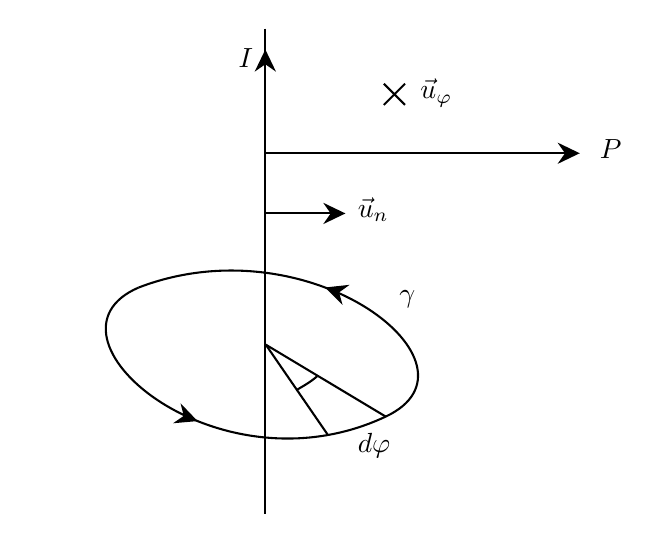
\begin{tikzpicture}[x=0.75pt,y=0.75pt,yscale=-1,xscale=1]
	%uncomment if require: \path (0,300); %set diagram left start at 0, and has height of 300

	%Straight Lines [id:da9211068985865756] 
	\draw    (220,49) -- (220,283) ;
	%Straight Lines [id:da36112272009272406] 
	\draw    (220,103.4) -- (220,62) ;
	\draw [shift={(220,59)}, rotate = 450] [fill={rgb, 255:red, 0; green, 0; blue, 0 }  ][line width=0.08]  [draw opacity=0] (10.72,-5.15) -- (0,0) -- (10.72,5.15) -- (7.12,0) -- cycle    ;
	%Straight Lines [id:da06976981758467105] 
	\draw    (220,109) -- (368.5,109) ;
	\draw [shift={(371.5,109)}, rotate = 180] [fill={rgb, 255:red, 0; green, 0; blue, 0 }  ][line width=0.08]  [draw opacity=0] (10.72,-5.15) -- (0,0) -- (10.72,5.15) -- (7.12,0) -- cycle    ;
	%Straight Lines [id:da477050807121032] 
	\draw    (220,138) -- (255.6,138) ;
	\draw [shift={(258.6,138)}, rotate = 180] [fill={rgb, 255:red, 0; green, 0; blue, 0 }  ][line width=0.08]  [draw opacity=0] (10.72,-5.15) -- (0,0) -- (10.72,5.15) -- (7.12,0) -- cycle    ;
	\draw   (277.1,75.5) -- (287.3,85.7)(287.3,75.5) -- (277.1,85.7) ;
	%Curve Lines [id:da009775526404201873] 
	\draw    (159,173.68) .. controls (242,141.83) and (330,211.6) .. (278,235.87) ;
	\draw [shift={(248.81,173.68)}, rotate = 19.39] [fill={rgb, 255:red, 0; green, 0; blue, 0 }  ][line width=0.08]  [draw opacity=0] (10.72,-5.15) -- (0,0) -- (10.72,5.15) -- (7.12,0) -- cycle    ;
	%Curve Lines [id:da9385892682251267] 
	\draw    (278,235.87) .. controls (196,274.55) and (106,196.43) .. (159,173.68) ;
	\draw [shift={(187.37,238.04)}, rotate = 200.57] [fill={rgb, 255:red, 0; green, 0; blue, 0 }  ][line width=0.08]  [draw opacity=0] (10.72,-5.15) -- (0,0) -- (10.72,5.15) -- (7.12,0) -- cycle    ;
	%Straight Lines [id:da9153580905085494] 
	\draw    (220.2,201.2) -- (278,235.87) ;
	%Straight Lines [id:da722540916164276] 
	\draw    (220.2,201.2) -- (250.2,244.8) ;
	%Curve Lines [id:da7608604455030328] 
	\draw    (235.2,223) .. controls (237.4,221.6) and (241.4,219.6) .. (245,216.4) ;

	% Text Node
	\draw (210.6,63.2) node    {$I$};
	% Text Node
	\draw (386.4,107.2) node    {$P$};
	% Text Node
	\draw (272,136) node    {$\vec{u}_{n}$};
	% Text Node
	\draw (302.4,80) node    {$\vec{u}_{\varphi }$};
	% Text Node
	\draw (288.4,179.2) node    {$\gamma $};
	% Text Node
	\draw (272.4,250) node    {$d\varphi $};

	\end{tikzpicture}
\end{figure}
\FloatBarrier

Introduciamo un sistema di riferimento in coordinate cilindriche in cui ogni punto è determinato da $ P=P(z,R,\varphi) $.
Abbiamo che

\[
	d\vec{l} = dz\;\vec{u}_z + dR\;\vec{u}_n + Rd\varphi \; \vec{u}_{\varphi}
\]

Calcoliamo la circuitazione di $\vec{B}$

\[
	\oint_{\gamma} \vec{B} \cdot d\vec{l} =\oint_{\gamma} \frac{\mu_0 I}{2\pi R}\vec{u}_{\varphi} \; [dz\;\vec{u}_z + dR\;\vec{u}_n + Rd\varphi \; \vec{u}_{\varphi}] = \oint_{\gamma} \frac{\mu_0 I}{2\pi R}Rd\varphi
\]

Dove abbiamo usato le proprietà del prodotto scalare e la formula per il campo magnetico prodotto da un filo percorso da corrente. Quindi

\[
	\oint_{\gamma} \vec{B} \cdot d\vec{l} = \frac{\mu_0 I}{2\pi}\oint_{\gamma} d\varphi = \frac{\mu_0 I}{2\pi} \cdot 2\pi = \mu_0 I
\]

Introduciamo anche il concetto di \emph{ordine di concatenazione}, nel senso che una linea $\gamma$ può avvolgersi $n$ volte attorno al filo percorso da corrente.

\begin{figure}[htpb]
	\centering

	\tikzset{every picture/.style={line width=0.75pt}} %set default line width to 0.75pt        

	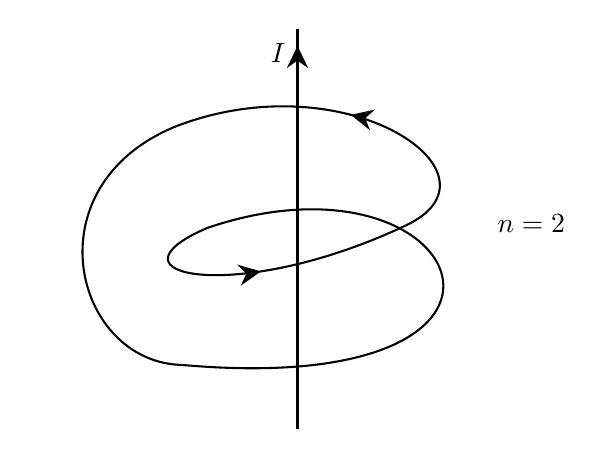
\begin{tikzpicture}[x=0.75pt,y=0.75pt,yscale=-1,xscale=1]
	%uncomment if require: \path (0,300); %set diagram left start at 0, and has height of 300

	%Straight Lines [id:da7476669646127272] 
	\draw    (252,49) -- (252,242) ;
	%Straight Lines [id:da29768359794142274] 
	\draw    (252,93.87) -- (252,60.25) ;
	\draw [shift={(252,57.25)}, rotate = 450] [fill={rgb, 255:red, 0; green, 0; blue, 0 }  ][line width=0.08]  [draw opacity=0] (10.72,-5.15) -- (0,0) -- (10.72,5.15) -- (7.12,0) -- cycle    ;
	%Curve Lines [id:da3466057001566656] 
	\draw    (193.5,96) .. controls (276.5,64.15) and (356,119.6) .. (304,143.87) ;
	\draw [shift={(277.71,90.5)}, rotate = 13.28] [fill={rgb, 255:red, 0; green, 0; blue, 0 }  ][line width=0.08]  [draw opacity=0] (10.72,-5.15) -- (0,0) -- (10.72,5.15) -- (7.12,0) -- cycle    ;
	%Curve Lines [id:da9829470547669434] 
	\draw    (208.5,145) .. controls (334.5,102) and (388.5,228) .. (196.5,211) ;
	%Curve Lines [id:da1539438051158717] 
	\draw    (304,143.87) .. controls (222,182.55) and (155.5,167.75) .. (208.5,145) ;
	\draw [shift={(234.37,165.93)}, rotate = 170.42] [fill={rgb, 255:red, 0; green, 0; blue, 0 }  ][line width=0.08]  [draw opacity=0] (10.72,-5.15) -- (0,0) -- (10.72,5.15) -- (7.12,0) -- cycle    ;
	%Curve Lines [id:da9265603983516404] 
	\draw    (193.5,96) .. controls (122.5,125) and (144.5,210) .. (196.5,211) ;

	% Text Node
	\draw (242.6,60.71) node    {$I$};
	% Text Node
	\draw (364.6,142.71) node    {$n=2$};

	\end{tikzpicture}
\end{figure}
\FloatBarrier

In tal caso

\[
	\oint_{\gamma} \vec{B} \cdot d\vec{l} = n\;\mu_0 I
\]

Precisiamo il segno da usare per le correnti

\begin{itemize}
	\item $ I>0 $ se concorde al verso di $\gamma$
	\item $ I<0 $ se discorde al verso di $\gamma$
\end{itemize}

Se la corrente non risulta concatenata a $\gamma$ i contributi mentre si integra l'angolo $\varphi$ si cancellano.

\begin{figure}[htpb]
	\centering

	\tikzset{every picture/.style={line width=0.75pt}} %set default line width to 0.75pt        

	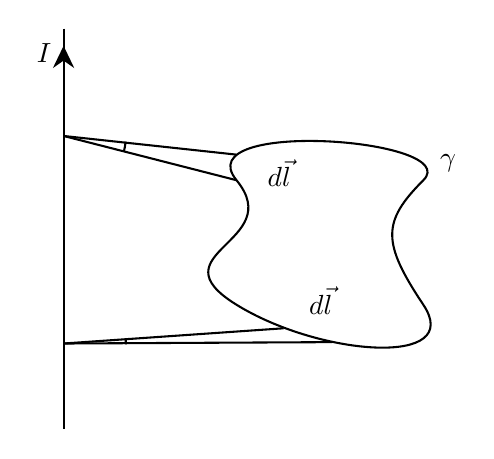
\begin{tikzpicture}[x=0.75pt,y=0.75pt,yscale=-1,xscale=1]
	%uncomment if require: \path (0,300); %set diagram left start at 0, and has height of 300

	%Straight Lines [id:da40927297486999903] 
	\draw    (225,69) -- (225,262) ;
	%Straight Lines [id:da8720550292630895] 
	\draw    (225,113.87) -- (225,80.25) ;
	\draw [shift={(225,77.25)}, rotate = 450] [fill={rgb, 255:red, 0; green, 0; blue, 0 }  ][line width=0.08]  [draw opacity=0] (10.72,-5.15) -- (0,0) -- (10.72,5.15) -- (7.12,0) -- cycle    ;
	%Shape: Polygon Curved [id:ds3996198548298875] 
	\draw   (308.33,142) .. controls (283.83,112) and (418.33,122) .. (398.33,142) .. controls (378.33,162) and (378.33,172) .. (398.33,202) .. controls (418.33,232) and (348.83,227) .. (308.33,202) .. controls (267.83,177) and (332.83,172) .. (308.33,142) -- cycle ;
	%Straight Lines [id:da21112185649434645] 
	\draw    (308.33,129.67) -- (225,120.67) ;
	%Straight Lines [id:da4371563579602411] 
	\draw    (308.33,142) -- (225,120.67) ;
	%Straight Lines [id:da6581159860746844] 
	\draw    (331,213.33) -- (225,220.67) ;
	%Straight Lines [id:da7631853339077679] 
	\draw    (354.33,220) -- (225,220.67) ;
	%Shape: Arc [id:dp6176391255763463] 
	\draw  [draw opacity=0] (254.87,123.44) .. controls (254.72,125.1) and (254.43,126.72) .. (254.02,128.29) -- (225,120.67) -- cycle ; \draw   (254.87,123.44) .. controls (254.72,125.1) and (254.43,126.72) .. (254.02,128.29) ;
	%Shape: Arc [id:dp7056007805282605] 
	\draw  [draw opacity=0] (254.91,218.36) .. controls (254.97,219.12) and (255,219.89) .. (255,220.67) .. controls (255,220.8) and (255,220.94) .. (255,221.07) -- (225,220.67) -- cycle ; \draw   (254.91,218.36) .. controls (254.97,219.12) and (255,219.89) .. (255,220.67) .. controls (255,220.8) and (255,220.94) .. (255,221.07) ;

	% Text Node
	\draw (215.6,80.71) node    {$I$};
	% Text Node
	\draw (328.93,138.71) node    {$d\vec{l}$};
	% Text Node
	\draw (348.93,200.05) node    {$d\vec{l}$};
	% Text Node
	\draw (410.27,134.05) node    {$\gamma $};

	\end{tikzpicture}
\end{figure}
\FloatBarrier

Dal momento che $ \vec{B}  $ gode del principio di sovrapposizione degli effetti, si può considerare la somma delle correnti concatenate per generalizzare il concetto.

\begin{align*}
	\oint_{\gamma} \vec{B}_{\text{tot}}\cdot d\vec{l} &=  \oint_{\gamma} (\Sigma_i\vec{B}_i  ) \cdot d\vec{l} \\
	&= \Sigma_i \oint_{\gamma} \vec{B}_i\cdot d\vec{l} \\
	&= \Sigma_i \; \mu_0 I_i^{\text{concatenata a}\gamma} \\
	&= \mu_0 I_{\text{tot}}^{\text{concatenata a}\gamma}
\end{align*}

Possiamo quindi enunciare la legge di Ampere

\[
	\boxed{\oint_{\gamma} \vec{B} \cdot d\vec{l} = \mu_0 I^{\text{concatenata a}\gamma}_{\text{tot}}}
\]

Vale anche se il circuito non è rettilineo.

\subsection{IV Equazione di Maxwell}

Consideriamo una situazione in regime stazionario, quindi con la corrente costante in tutto il circuito.

Definiamo $\vec{J}$ anche all'esterno dei fili, ossia $\vec{J}=0$ in assenza di corrente.

\begin{figure}[htpb]
	\centering

	\tikzset{every picture/.style={line width=0.75pt}} %set default line width to 0.75pt        

	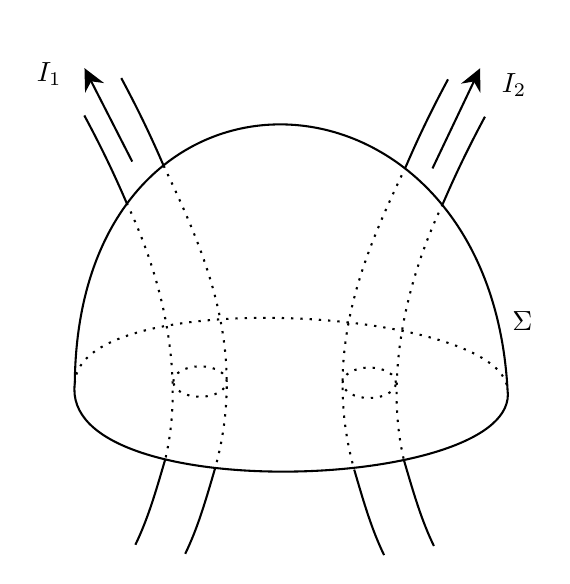
\begin{tikzpicture}[x=0.75pt,y=0.75pt,yscale=-1,xscale=1]
	%uncomment if require: \path (0,300); %set diagram left start at 0, and has height of 300

	%Curve Lines [id:da9285892682977372] 
	\draw    (189,190) .. controls (181.5,250) and (404.5,242) .. (397.5,193) ;
	%Curve Lines [id:da7924907437346282] 
	\draw  [dash pattern={on 0.84pt off 2.51pt}]  (189,190) .. controls (190.5,142) and (395.5,153) .. (397.5,193) ;
	%Curve Lines [id:da020508186457237843] 
	\draw    (189,190) .. controls (190.5,19) and (388.5,27) .. (397.5,193) ;
	%Curve Lines [id:da7775810360309536] 
	\draw  [dash pattern={on 0.84pt off 2.51pt}]  (214,103) .. controls (233.5,144) and (241.4,189.2) .. (232.6,226.4) ;
	%Shape: Ellipse [id:dp5111089961649995] 
	\draw  [dash pattern={on 0.84pt off 2.51pt}] (236.5,189) .. controls (236.5,184.94) and (242.25,181.66) .. (249.35,181.66) .. controls (256.45,181.66) and (262.2,184.94) .. (262.2,189) .. controls (262.2,193.06) and (256.45,196.34) .. (249.35,196.34) .. controls (242.25,196.34) and (236.5,193.06) .. (236.5,189) -- cycle ;
	%Curve Lines [id:da5839381113347033] 
	\draw  [dash pattern={on 0.84pt off 2.51pt}]  (231.8,85) .. controls (251.3,126) and (272.6,173.2) .. (256.6,230.8) ;
	%Curve Lines [id:da4469723860447563] 
	\draw    (211.4,42.8) .. controls (220.2,59.2) and (226.2,72) .. (231.8,85) ;
	%Curve Lines [id:da6134223361402396] 
	\draw    (193.6,60.8) .. controls (202.4,77.2) and (208.4,90) .. (214,103) ;
	%Curve Lines [id:da4664167643230339] 
	\draw    (232.6,226.4) .. controls (227.8,242.8) and (224.2,255.2) .. (218.2,267.6) ;
	%Curve Lines [id:da13402819752656003] 
	\draw    (256.6,230.8) .. controls (251.8,247.2) and (248.2,259.6) .. (242.2,272) ;
	%Curve Lines [id:da559353079188736] 
	\draw  [dash pattern={on 0.84pt off 2.51pt}]  (366.22,103.6) .. controls (346.72,144.6) and (338.82,189.8) .. (347.62,227) ;
	%Shape: Ellipse [id:dp7162312556907064] 
	\draw  [dash pattern={on 0.84pt off 2.51pt}] (343.72,189.6) .. controls (343.72,185.54) and (337.97,182.26) .. (330.87,182.26) .. controls (323.77,182.26) and (318.02,185.54) .. (318.02,189.6) .. controls (318.02,193.66) and (323.77,196.94) .. (330.87,196.94) .. controls (337.97,196.94) and (343.72,193.66) .. (343.72,189.6) -- cycle ;
	%Curve Lines [id:da3010331939362052] 
	\draw  [dash pattern={on 0.84pt off 2.51pt}]  (348.42,85.6) .. controls (328.92,126.6) and (307.62,173.8) .. (323.62,231.4) ;
	%Curve Lines [id:da4468898215223951] 
	\draw    (368.82,43.4) .. controls (360.02,59.8) and (354.02,72.6) .. (348.42,85.6) ;
	%Curve Lines [id:da9455644848772078] 
	\draw    (386.62,61.4) .. controls (377.82,77.8) and (371.82,90.6) .. (366.22,103.6) ;
	%Curve Lines [id:da9875240906730798] 
	\draw    (347.62,227) .. controls (352.42,243.4) and (356.02,255.8) .. (362.02,268.2) ;
	%Curve Lines [id:da7459083423841357] 
	\draw    (323.62,231.4) .. controls (328.42,247.8) and (332.02,260.2) .. (338.02,272.6) ;
	%Straight Lines [id:da20399307729549032] 
	\draw    (216.67,83) -- (195.03,40.67) ;
	\draw [shift={(193.67,38)}, rotate = 422.93] [fill={rgb, 255:red, 0; green, 0; blue, 0 }  ][line width=0.08]  [draw opacity=0] (10.72,-5.15) -- (0,0) -- (10.72,5.15) -- (7.12,0) -- cycle    ;
	%Straight Lines [id:da20561143386928005] 
	\draw    (361.33,86.33) -- (383.04,40.71) ;
	\draw [shift={(384.33,38)}, rotate = 475.45] [fill={rgb, 255:red, 0; green, 0; blue, 0 }  ][line width=0.08]  [draw opacity=0] (10.72,-5.15) -- (0,0) -- (10.72,5.15) -- (7.12,0) -- cycle    ;

	% Text Node
	\draw (404.67,160) node    {$\Sigma $};
	% Text Node
	\draw (176.67,40.67) node    {$I_{1}$};
	% Text Node
	\draw (400.67,46) node    {$I_{2}$};

	\end{tikzpicture}
\end{figure}
\FloatBarrier

Ora ricordando che

\[
	I_{\text{tot}}^{\text{conc. a}\gamma} = \int_{\Sigma}\vec{J} \cdot \vec{n} dS
\]

Possiamo riscrivere la legge di Ampere e applicare il teorema di Stokes

\begin{align*}
	\oint_{\gamma} \vec{B} \cdot d\vec{l} &= \mu_0 \; I^{\text{conc. a}\gamma}_{\text{tot}}  \\
	\oint_{\gamma} \vec{B} \cdot d\vec{l} &= \mu_0 \int_{\Sigma}\vec{J} \cdot \vec{n} dS \\
	\int_{\Sigma} \text{rot}\vec{B} \cdot \vec{n} dS &=  \int_{\Sigma}\mu_0\vec{J} \cdot \vec{n} dS
\end{align*}

Ma dal momento che non abbiamo fatto supposizioni di alcun tipo sulla forma possiamo concludere la \textbf{IV Equazione di Maxwell}

\[
	\boxed{\text{rot}\vec{B} =\mu_0 \vec{J}}
\]

Valida solo in regime stazionario.

Ne deduciamo che $ \vec{B}  $ non è conservativo, non essendo irrotazionale, infatti presenta delle linee chiuse.

Le linee di $\vec{B}$ descrivono un vortice e la corrente sta nel suo centro. L'operatore rotore comunica qualcosa sulla geometria del campo, perché è non nullo nei punti che sono al centro dei vortici delle linee di flusso. Il rotore inoltre ci informa anche sull'asse attorno al quale le linee stanno ruotando e quindi il piano in cui esse descrivono i percorsi chiusi.

Il $ \text{rot}\vec{B}  $ è $ \neq 0 $ nei punti in cui sono presenti dei vortici e ci dice l'orientazione di questi vortici.

N.B.

\[
	\begin{array}{c}
		\text{rot} \vec{v} =0 \\
		\text{div} \vec{v} =0
	\end{array}
	\iff \vec{v} =0
\]

A riprova che la IV Equazione di Maxwell vale implica che ci si trovi in regime stazionario ($ \text{div}\vec{J} =0 $ ), possiamo applicare la divergenza a entrambi i termini, ricordando l'identità operatoriale $ \text{div}(\text{rot}\vec{v} )=0 $

\begin{align*}
	\text{rot}\vec{B}  &= \mu_0 \vec{J}  \\
	\text{div}(\text{rot}\vec{B} ) &=  \text{div}(\mu_0\vec{J} ) \\
	0= \text{div}(\text{rot}\vec{B} ) &= \mu_0 \text{div}\vec{J} \implies \text{div}\vec{J} =0
\end{align*}

\section{Condizioni al contorno di B}

Abbiamo visto che il campo elettrostatico è discontinuo nell'attraversamento di una superficie carica. Analogamente dimostriamo che il campo magnetico è discontinuo nell'attraversamento di una superficie sede di correnti. Non possiamo usare il vettore $\vec{J}$ per descrivere un vettore superficiale.

\begin{figure}[htpb]
	\centering

	\tikzset{every picture/.style={line width=0.75pt}} %set default line width to 0.75pt        

	\begin{tikzpicture}[x=0.75pt,y=0.75pt,yscale=-1,xscale=1]
	%uncomment if require: \path (0,300); %set diagram left start at 0, and has height of 300

	%Straight Lines [id:da40290349945353854] 
	\draw    (154,165) -- (483.5,165) ;
	%Shape: Circle [id:dp7722867521050865] 
	\draw  [fill={rgb, 255:red, 0; green, 0; blue, 0 }  ,fill opacity=1 ] (164.5,165) .. controls (164.5,164.31) and (165.06,163.75) .. (165.75,163.75) .. controls (166.44,163.75) and (167,164.31) .. (167,165) .. controls (167,165.69) and (166.44,166.25) .. (165.75,166.25) .. controls (165.06,166.25) and (164.5,165.69) .. (164.5,165) -- cycle ;
	%Straight Lines [id:da6036238931546025] 
	\draw    (299.99,165.11) -- (327.33,100.76) ;
	\draw [shift={(328.5,98)}, rotate = 473.01] [fill={rgb, 255:red, 0; green, 0; blue, 0 }  ][line width=0.08]  [draw opacity=0] (10.72,-5.15) -- (0,0) -- (10.72,5.15) -- (7.12,0) -- cycle    ;
	%Straight Lines [id:da876809805291892] 
	\draw    (234.5,230) -- (297.86,167.22) ;
	\draw [shift={(299.99,165.11)}, rotate = 495.26] [fill={rgb, 255:red, 0; green, 0; blue, 0 }  ][line width=0.08]  [draw opacity=0] (10.72,-5.15) -- (0,0) -- (10.72,5.15) -- (7.12,0) -- cycle    ;
	%Shape: Circle [id:dp10580150585865411] 
	\draw  [fill={rgb, 255:red, 0; green, 0; blue, 0 }  ,fill opacity=1 ] (184.5,165) .. controls (184.5,164.31) and (185.06,163.75) .. (185.75,163.75) .. controls (186.44,163.75) and (187,164.31) .. (187,165) .. controls (187,165.69) and (186.44,166.25) .. (185.75,166.25) .. controls (185.06,166.25) and (184.5,165.69) .. (184.5,165) -- cycle ;
	%Shape: Circle [id:dp15575276541461003] 
	\draw  [fill={rgb, 255:red, 0; green, 0; blue, 0 }  ,fill opacity=1 ] (204.5,165) .. controls (204.5,164.31) and (205.06,163.75) .. (205.75,163.75) .. controls (206.44,163.75) and (207,164.31) .. (207,165) .. controls (207,165.69) and (206.44,166.25) .. (205.75,166.25) .. controls (205.06,166.25) and (204.5,165.69) .. (204.5,165) -- cycle ;
	%Shape: Circle [id:dp7242236667809356] 
	\draw  [fill={rgb, 255:red, 0; green, 0; blue, 0 }  ,fill opacity=1 ] (224.5,165) .. controls (224.5,164.31) and (225.06,163.75) .. (225.75,163.75) .. controls (226.44,163.75) and (227,164.31) .. (227,165) .. controls (227,165.69) and (226.44,166.25) .. (225.75,166.25) .. controls (225.06,166.25) and (224.5,165.69) .. (224.5,165) -- cycle ;
	%Shape: Circle [id:dp19764606296007692] 
	\draw  [fill={rgb, 255:red, 0; green, 0; blue, 0 }  ,fill opacity=1 ] (244.5,165) .. controls (244.5,164.31) and (245.06,163.75) .. (245.75,163.75) .. controls (246.44,163.75) and (247,164.31) .. (247,165) .. controls (247,165.69) and (246.44,166.25) .. (245.75,166.25) .. controls (245.06,166.25) and (244.5,165.69) .. (244.5,165) -- cycle ;
	%Shape: Circle [id:dp9900072173023722] 
	\draw  [fill={rgb, 255:red, 0; green, 0; blue, 0 }  ,fill opacity=1 ] (264.5,165) .. controls (264.5,164.31) and (265.06,163.75) .. (265.75,163.75) .. controls (266.44,163.75) and (267,164.31) .. (267,165) .. controls (267,165.69) and (266.44,166.25) .. (265.75,166.25) .. controls (265.06,166.25) and (264.5,165.69) .. (264.5,165) -- cycle ;
	%Shape: Circle [id:dp24295923777511308] 
	\draw  [fill={rgb, 255:red, 0; green, 0; blue, 0 }  ,fill opacity=1 ] (284.5,165) .. controls (284.5,164.31) and (285.06,163.75) .. (285.75,163.75) .. controls (286.44,163.75) and (287,164.31) .. (287,165) .. controls (287,165.69) and (286.44,166.25) .. (285.75,166.25) .. controls (285.06,166.25) and (284.5,165.69) .. (284.5,165) -- cycle ;
	%Shape: Circle [id:dp5824761646667302] 
	\draw  [fill={rgb, 255:red, 0; green, 0; blue, 0 }  ,fill opacity=1 ] (304.5,165) .. controls (304.5,164.31) and (305.06,163.75) .. (305.75,163.75) .. controls (306.44,163.75) and (307,164.31) .. (307,165) .. controls (307,165.69) and (306.44,166.25) .. (305.75,166.25) .. controls (305.06,166.25) and (304.5,165.69) .. (304.5,165) -- cycle ;
	%Shape: Circle [id:dp3131757951408054] 
	\draw  [fill={rgb, 255:red, 0; green, 0; blue, 0 }  ,fill opacity=1 ] (324.5,165) .. controls (324.5,164.31) and (325.06,163.75) .. (325.75,163.75) .. controls (326.44,163.75) and (327,164.31) .. (327,165) .. controls (327,165.69) and (326.44,166.25) .. (325.75,166.25) .. controls (325.06,166.25) and (324.5,165.69) .. (324.5,165) -- cycle ;
	%Shape: Circle [id:dp3016076811973367] 
	\draw  [fill={rgb, 255:red, 0; green, 0; blue, 0 }  ,fill opacity=1 ] (344.5,165) .. controls (344.5,164.31) and (345.06,163.75) .. (345.75,163.75) .. controls (346.44,163.75) and (347,164.31) .. (347,165) .. controls (347,165.69) and (346.44,166.25) .. (345.75,166.25) .. controls (345.06,166.25) and (344.5,165.69) .. (344.5,165) -- cycle ;
	%Shape: Circle [id:dp35138916967723177] 
	\draw  [fill={rgb, 255:red, 0; green, 0; blue, 0 }  ,fill opacity=1 ] (364.5,165) .. controls (364.5,164.31) and (365.06,163.75) .. (365.75,163.75) .. controls (366.44,163.75) and (367,164.31) .. (367,165) .. controls (367,165.69) and (366.44,166.25) .. (365.75,166.25) .. controls (365.06,166.25) and (364.5,165.69) .. (364.5,165) -- cycle ;
	%Shape: Circle [id:dp5071323612099659] 
	\draw  [fill={rgb, 255:red, 0; green, 0; blue, 0 }  ,fill opacity=1 ] (384.5,165) .. controls (384.5,164.31) and (385.06,163.75) .. (385.75,163.75) .. controls (386.44,163.75) and (387,164.31) .. (387,165) .. controls (387,165.69) and (386.44,166.25) .. (385.75,166.25) .. controls (385.06,166.25) and (384.5,165.69) .. (384.5,165) -- cycle ;
	%Shape: Circle [id:dp09177828943056299] 
	\draw  [fill={rgb, 255:red, 0; green, 0; blue, 0 }  ,fill opacity=1 ] (404.5,165) .. controls (404.5,164.31) and (405.06,163.75) .. (405.75,163.75) .. controls (406.44,163.75) and (407,164.31) .. (407,165) .. controls (407,165.69) and (406.44,166.25) .. (405.75,166.25) .. controls (405.06,166.25) and (404.5,165.69) .. (404.5,165) -- cycle ;
	%Shape: Circle [id:dp9193795776307525] 
	\draw  [fill={rgb, 255:red, 0; green, 0; blue, 0 }  ,fill opacity=1 ] (424.5,165) .. controls (424.5,164.31) and (425.06,163.75) .. (425.75,163.75) .. controls (426.44,163.75) and (427,164.31) .. (427,165) .. controls (427,165.69) and (426.44,166.25) .. (425.75,166.25) .. controls (425.06,166.25) and (424.5,165.69) .. (424.5,165) -- cycle ;
	%Shape: Circle [id:dp27302929469440107] 
	\draw  [fill={rgb, 255:red, 0; green, 0; blue, 0 }  ,fill opacity=1 ] (444.5,165) .. controls (444.5,164.31) and (445.06,163.75) .. (445.75,163.75) .. controls (446.44,163.75) and (447,164.31) .. (447,165) .. controls (447,165.69) and (446.44,166.25) .. (445.75,166.25) .. controls (445.06,166.25) and (444.5,165.69) .. (444.5,165) -- cycle ;
	%Shape: Circle [id:dp48175179756314135] 
	\draw  [fill={rgb, 255:red, 0; green, 0; blue, 0 }  ,fill opacity=1 ] (464.5,165) .. controls (464.5,164.31) and (465.06,163.75) .. (465.75,163.75) .. controls (466.44,163.75) and (467,164.31) .. (467,165) .. controls (467,165.69) and (466.44,166.25) .. (465.75,166.25) .. controls (465.06,166.25) and (464.5,165.69) .. (464.5,165) -- cycle ;

	% Text Node
	\draw (134,135) node    {$1$};
	% Text Node
	\draw (134,196) node    {$2$};
	% Text Node
	\draw (348.67,101.33) node    {$\vec{B}_{1}$};
	% Text Node
	\draw (269,223) node    {$\vec{B}_{2}$};
	% Text Node
	\draw (498.67,165) node    {$\Sigma $};
	% Text Node
	\draw (402.67,147.8) node    {$j_{s}$};

	\end{tikzpicture}
\end{figure}
\FloatBarrier

Se consideriamo un tratto $dl$ sulla superficie, possiamo pensare che su di esso stia scorrendo della corrente e introdurre una nuova quantità che indichiamo come \textbf{densità di corrente superficiale} pari al rapporto della corrente $di$ sulla lunghezza $dl$.

\[
	\boxed{j_s = \frac{di}{dl}}
\]

Per determinare le condizioni per la componente normale consideriamo un cilindro di area $dS$ e altezza $dh$ a ridosso della superficie di separazione dei due mezzi. Sia $dh \ll \sqrt{dS}$ in modo da trascurare il flusso laterale.

\begin{figure}[htpb]
	\centering

	\tikzset{every picture/.style={line width=0.75pt}} %set default line width to 0.75pt        

	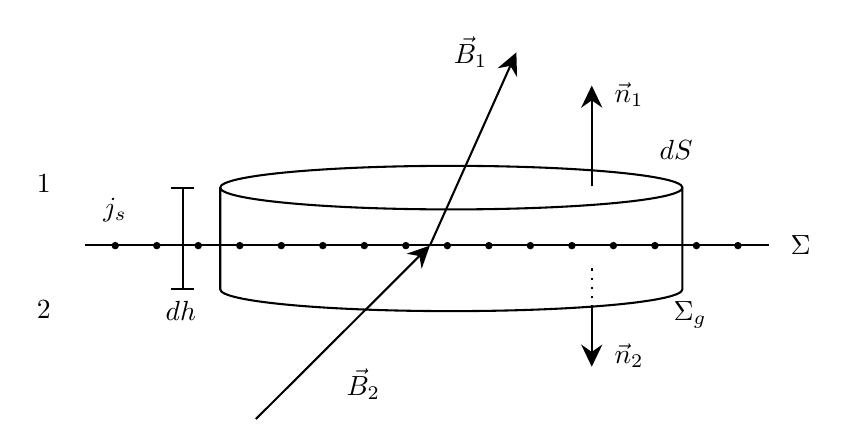
\begin{tikzpicture}[x=0.75pt,y=0.75pt,yscale=-1,xscale=1]
	%uncomment if require: \path (0,300); %set diagram left start at 0, and has height of 300

	%Straight Lines [id:da6213004317923272] 
	\draw    (159.33,194.33) -- (488.83,194.33) ;
	%Straight Lines [id:da7110584731917358] 
	\draw    (325.33,194.44) -- (365.77,104.07) ;
	\draw [shift={(367,101.33)}, rotate = 474.11] [fill={rgb, 255:red, 0; green, 0; blue, 0 }  ][line width=0.08]  [draw opacity=0] (10.72,-5.15) -- (0,0) -- (10.72,5.15) -- (7.12,0) -- cycle    ;
	%Shape: Can [id:dp8536022843616089] 
	\draw   (447,166.5) -- (447,215.5) .. controls (447,221.3) and (397.15,226) .. (335.67,226) .. controls (274.18,226) and (224.33,221.3) .. (224.33,215.5) -- (224.33,166.5) .. controls (224.33,160.7) and (274.18,156) .. (335.67,156) .. controls (397.15,156) and (447,160.7) .. (447,166.5) .. controls (447,172.3) and (397.15,177) .. (335.67,177) .. controls (274.18,177) and (224.33,172.3) .. (224.33,166.5) ;
	%Straight Lines [id:da4110358980175308] 
	\draw    (206.33,215.5) -- (206.33,166.5) ;
	\draw [shift={(206.33,166.5)}, rotate = 450] [color={rgb, 255:red, 0; green, 0; blue, 0 }  ][line width=0.75]    (0,5.59) -- (0,-5.59)   ;
	\draw [shift={(206.33,215.5)}, rotate = 450] [color={rgb, 255:red, 0; green, 0; blue, 0 }  ][line width=0.75]    (0,5.59) -- (0,-5.59)   ;
	%Straight Lines [id:da410379630838986] 
	\draw    (403.33,165.77) -- (403.33,120.33) ;
	\draw [shift={(403.33,117.33)}, rotate = 450] [fill={rgb, 255:red, 0; green, 0; blue, 0 }  ][line width=0.08]  [draw opacity=0] (10.72,-5.15) -- (0,0) -- (10.72,5.15) -- (7.12,0) -- cycle    ;
	%Straight Lines [id:da8371791645883637] 
	\draw    (403.33,249.77) -- (403.33,224.33) ;
	\draw [shift={(403.33,252.77)}, rotate = 270] [fill={rgb, 255:red, 0; green, 0; blue, 0 }  ][line width=0.08]  [draw opacity=0] (10.72,-5.15) -- (0,0) -- (10.72,5.15) -- (7.12,0) -- cycle    ;
	%Straight Lines [id:da24523180797428168] 
	\draw  [dash pattern={on 0.84pt off 2.51pt}]  (403.33,224.33) -- (403.33,204.33) ;
	%Straight Lines [id:da5308318657083659] 
	\draw    (241.5,278) -- (323.2,196.56) ;
	\draw [shift={(325.33,194.44)}, rotate = 495.09] [fill={rgb, 255:red, 0; green, 0; blue, 0 }  ][line width=0.08]  [draw opacity=0] (10.72,-5.15) -- (0,0) -- (10.72,5.15) -- (7.12,0) -- cycle    ;
	%Shape: Circle [id:dp16041020967866237] 
	\draw  [fill={rgb, 255:red, 0; green, 0; blue, 0 }  ,fill opacity=1 ] (172.5,194.44) .. controls (172.5,193.75) and (173.06,193.19) .. (173.75,193.19) .. controls (174.44,193.19) and (175,193.75) .. (175,194.44) .. controls (175,195.13) and (174.44,195.69) .. (173.75,195.69) .. controls (173.06,195.69) and (172.5,195.13) .. (172.5,194.44) -- cycle ;
	%Shape: Circle [id:dp8427889866553417] 
	\draw  [fill={rgb, 255:red, 0; green, 0; blue, 0 }  ,fill opacity=1 ] (192.5,194.44) .. controls (192.5,193.75) and (193.06,193.19) .. (193.75,193.19) .. controls (194.44,193.19) and (195,193.75) .. (195,194.44) .. controls (195,195.13) and (194.44,195.69) .. (193.75,195.69) .. controls (193.06,195.69) and (192.5,195.13) .. (192.5,194.44) -- cycle ;
	%Shape: Circle [id:dp6742655422084851] 
	\draw  [fill={rgb, 255:red, 0; green, 0; blue, 0 }  ,fill opacity=1 ] (212.5,194.44) .. controls (212.5,193.75) and (213.06,193.19) .. (213.75,193.19) .. controls (214.44,193.19) and (215,193.75) .. (215,194.44) .. controls (215,195.13) and (214.44,195.69) .. (213.75,195.69) .. controls (213.06,195.69) and (212.5,195.13) .. (212.5,194.44) -- cycle ;
	%Shape: Circle [id:dp2559509551421366] 
	\draw  [fill={rgb, 255:red, 0; green, 0; blue, 0 }  ,fill opacity=1 ] (232.5,194.44) .. controls (232.5,193.75) and (233.06,193.19) .. (233.75,193.19) .. controls (234.44,193.19) and (235,193.75) .. (235,194.44) .. controls (235,195.13) and (234.44,195.69) .. (233.75,195.69) .. controls (233.06,195.69) and (232.5,195.13) .. (232.5,194.44) -- cycle ;
	%Shape: Circle [id:dp25389345637442107] 
	\draw  [fill={rgb, 255:red, 0; green, 0; blue, 0 }  ,fill opacity=1 ] (252.5,194.44) .. controls (252.5,193.75) and (253.06,193.19) .. (253.75,193.19) .. controls (254.44,193.19) and (255,193.75) .. (255,194.44) .. controls (255,195.13) and (254.44,195.69) .. (253.75,195.69) .. controls (253.06,195.69) and (252.5,195.13) .. (252.5,194.44) -- cycle ;
	%Shape: Circle [id:dp25508561739913915] 
	\draw  [fill={rgb, 255:red, 0; green, 0; blue, 0 }  ,fill opacity=1 ] (272.5,194.44) .. controls (272.5,193.75) and (273.06,193.19) .. (273.75,193.19) .. controls (274.44,193.19) and (275,193.75) .. (275,194.44) .. controls (275,195.13) and (274.44,195.69) .. (273.75,195.69) .. controls (273.06,195.69) and (272.5,195.13) .. (272.5,194.44) -- cycle ;
	%Shape: Circle [id:dp44631343518992095] 
	\draw  [fill={rgb, 255:red, 0; green, 0; blue, 0 }  ,fill opacity=1 ] (292.5,194.44) .. controls (292.5,193.75) and (293.06,193.19) .. (293.75,193.19) .. controls (294.44,193.19) and (295,193.75) .. (295,194.44) .. controls (295,195.13) and (294.44,195.69) .. (293.75,195.69) .. controls (293.06,195.69) and (292.5,195.13) .. (292.5,194.44) -- cycle ;
	%Shape: Circle [id:dp5911616852292005] 
	\draw  [fill={rgb, 255:red, 0; green, 0; blue, 0 }  ,fill opacity=1 ] (312.5,194.44) .. controls (312.5,193.75) and (313.06,193.19) .. (313.75,193.19) .. controls (314.44,193.19) and (315,193.75) .. (315,194.44) .. controls (315,195.13) and (314.44,195.69) .. (313.75,195.69) .. controls (313.06,195.69) and (312.5,195.13) .. (312.5,194.44) -- cycle ;
	%Shape: Circle [id:dp10546600814340201] 
	\draw  [fill={rgb, 255:red, 0; green, 0; blue, 0 }  ,fill opacity=1 ] (332.5,194.44) .. controls (332.5,193.75) and (333.06,193.19) .. (333.75,193.19) .. controls (334.44,193.19) and (335,193.75) .. (335,194.44) .. controls (335,195.13) and (334.44,195.69) .. (333.75,195.69) .. controls (333.06,195.69) and (332.5,195.13) .. (332.5,194.44) -- cycle ;
	%Shape: Circle [id:dp13547297521940904] 
	\draw  [fill={rgb, 255:red, 0; green, 0; blue, 0 }  ,fill opacity=1 ] (352.5,194.44) .. controls (352.5,193.75) and (353.06,193.19) .. (353.75,193.19) .. controls (354.44,193.19) and (355,193.75) .. (355,194.44) .. controls (355,195.13) and (354.44,195.69) .. (353.75,195.69) .. controls (353.06,195.69) and (352.5,195.13) .. (352.5,194.44) -- cycle ;
	%Shape: Circle [id:dp09508956969941629] 
	\draw  [fill={rgb, 255:red, 0; green, 0; blue, 0 }  ,fill opacity=1 ] (372.5,194.44) .. controls (372.5,193.75) and (373.06,193.19) .. (373.75,193.19) .. controls (374.44,193.19) and (375,193.75) .. (375,194.44) .. controls (375,195.13) and (374.44,195.69) .. (373.75,195.69) .. controls (373.06,195.69) and (372.5,195.13) .. (372.5,194.44) -- cycle ;
	%Shape: Circle [id:dp7963240077414149] 
	\draw  [fill={rgb, 255:red, 0; green, 0; blue, 0 }  ,fill opacity=1 ] (392.5,194.44) .. controls (392.5,193.75) and (393.06,193.19) .. (393.75,193.19) .. controls (394.44,193.19) and (395,193.75) .. (395,194.44) .. controls (395,195.13) and (394.44,195.69) .. (393.75,195.69) .. controls (393.06,195.69) and (392.5,195.13) .. (392.5,194.44) -- cycle ;
	%Shape: Circle [id:dp7134148353618073] 
	\draw  [fill={rgb, 255:red, 0; green, 0; blue, 0 }  ,fill opacity=1 ] (412.5,194.44) .. controls (412.5,193.75) and (413.06,193.19) .. (413.75,193.19) .. controls (414.44,193.19) and (415,193.75) .. (415,194.44) .. controls (415,195.13) and (414.44,195.69) .. (413.75,195.69) .. controls (413.06,195.69) and (412.5,195.13) .. (412.5,194.44) -- cycle ;
	%Shape: Circle [id:dp6805815488388596] 
	\draw  [fill={rgb, 255:red, 0; green, 0; blue, 0 }  ,fill opacity=1 ] (432.5,194.44) .. controls (432.5,193.75) and (433.06,193.19) .. (433.75,193.19) .. controls (434.44,193.19) and (435,193.75) .. (435,194.44) .. controls (435,195.13) and (434.44,195.69) .. (433.75,195.69) .. controls (433.06,195.69) and (432.5,195.13) .. (432.5,194.44) -- cycle ;
	%Shape: Circle [id:dp751825076031954] 
	\draw  [fill={rgb, 255:red, 0; green, 0; blue, 0 }  ,fill opacity=1 ] (452.5,194.44) .. controls (452.5,193.75) and (453.06,193.19) .. (453.75,193.19) .. controls (454.44,193.19) and (455,193.75) .. (455,194.44) .. controls (455,195.13) and (454.44,195.69) .. (453.75,195.69) .. controls (453.06,195.69) and (452.5,195.13) .. (452.5,194.44) -- cycle ;
	%Shape: Circle [id:dp23506561777408042] 
	\draw  [fill={rgb, 255:red, 0; green, 0; blue, 0 }  ,fill opacity=1 ] (472.5,194.44) .. controls (472.5,193.75) and (473.06,193.19) .. (473.75,193.19) .. controls (474.44,193.19) and (475,193.75) .. (475,194.44) .. controls (475,195.13) and (474.44,195.69) .. (473.75,195.69) .. controls (473.06,195.69) and (472.5,195.13) .. (472.5,194.44) -- cycle ;

	% Text Node
	\draw (139.33,164.33) node    {$1$};
	% Text Node
	\draw (139.33,225.33) node    {$2$};
	% Text Node
	\draw (345,101.33) node    {$\vec{B}_{1}$};
	% Text Node
	\draw (293.33,261) node    {$\vec{B}_{2}$};
	% Text Node
	\draw (504,194.33) node    {$\Sigma $};
	% Text Node
	\draw (444,148.33) node    {$dS$};
	% Text Node
	\draw (205.33,225.67) node    {$dh$};
	% Text Node
	\draw (421.33,121.67) node    {$\vec{n}_{1}$};
	% Text Node
	\draw (421.33,247.33) node    {$\vec{n}_{2}$};
	% Text Node
	\draw (450.67,227.67) node    {$\Sigma _{g}$};
	% Text Node
	\draw (173.67,177.3) node    {$j_{s}$};

	\end{tikzpicture}
\end{figure}
\FloatBarrier

Ricordando che il flusso di $\vec{B}$ è sempre nullo su una superficie chiusa, possiamo scrivere

\begin{align*}
	0 = \Phi_{\Sigma g}(\vec{B} )  &\simeq  \vec{B}_1\cdot \vec{n}_1  dS + \vec{B}_2\cdot \vec{n}_2  dS    \\
	0 &= (\vec{B}_1\vec{n}_1 - \vec{B}_2\vec{n}_1 )dS \\
\end{align*}

Chiamando

\begin{gather*}
	B_{1n} = \vec{B}_1\cdot \vec{n}_1 \\
	B_{2n} = \vec{B}_2\cdot \vec{n}_1
\end{gather*}

Abbiamo

\[
	\boxed{B_{1n} = B_{2n}}
\]

Questo ci dice che la componente normale del campo magnetico si conserva.
Consideriamo a questo punto il versore tangente alla superficie e individuiamo un percorso chiuso $\gamma$ di forma rettangolare a cavallo della superficie, di altezza $dh$ e larghezza $dl$ con $ dh \ll dl $. Possiamo dire le seguenti cose.

\begin{figure}[htpb]
	\centering

	\tikzset{every picture/.style={line width=0.75pt}} %set default line width to 0.75pt        

	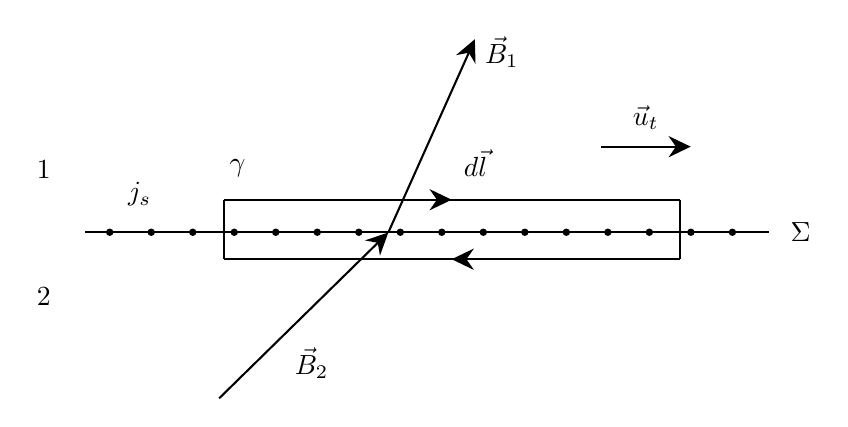
\begin{tikzpicture}[x=0.75pt,y=0.75pt,yscale=-1,xscale=1]
	%uncomment if require: \path (0,300); %set diagram left start at 0, and has height of 300

	%Straight Lines [id:da3977022913494037] 
	\draw    (174,185) -- (503.5,185) ;
	%Straight Lines [id:da7732099440082854] 
	\draw    (319.99,185.11) -- (360.44,94.74) ;
	\draw [shift={(361.67,92)}, rotate = 474.11] [fill={rgb, 255:red, 0; green, 0; blue, 0 }  ][line width=0.08]  [draw opacity=0] (10.72,-5.15) -- (0,0) -- (10.72,5.15) -- (7.12,0) -- cycle    ;
	%Straight Lines [id:da5500797242504052] 
	\draw    (240.67,169.33) -- (460.33,169.33) ;
	\draw [shift={(350.5,169.33)}, rotate = 180] [fill={rgb, 255:red, 0; green, 0; blue, 0 }  ][line width=0.08]  [draw opacity=0] (10.72,-5.15) -- (0,0) -- (10.72,5.15) -- (7.12,0) -- cycle    ;
	%Straight Lines [id:da6756783602076346] 
	\draw    (240.67,198) -- (460.33,198) ;
	\draw [shift={(350.5,198)}, rotate = 0] [fill={rgb, 255:red, 0; green, 0; blue, 0 }  ][line width=0.08]  [draw opacity=0] (10.72,-5.15) -- (0,0) -- (10.72,5.15) -- (7.12,0) -- cycle    ;
	%Straight Lines [id:da253951117937784] 
	\draw    (460.33,169.33) -- (460.33,198) ;
	%Straight Lines [id:da6384193071075221] 
	\draw    (240.67,169.33) -- (240.67,198) ;
	%Straight Lines [id:da29680057316531405] 
	\draw    (422.66,143.77) -- (462.67,143.77) ;
	\draw [shift={(465.67,143.77)}, rotate = 180] [fill={rgb, 255:red, 0; green, 0; blue, 0 }  ][line width=0.08]  [draw opacity=0] (10.72,-5.15) -- (0,0) -- (10.72,5.15) -- (7.12,0) -- cycle    ;
	%Straight Lines [id:da7403301396741371] 
	\draw    (238.5,265) -- (317.85,187.21) ;
	\draw [shift={(319.99,185.11)}, rotate = 495.57] [fill={rgb, 255:red, 0; green, 0; blue, 0 }  ][line width=0.08]  [draw opacity=0] (10.72,-5.15) -- (0,0) -- (10.72,5.15) -- (7.12,0) -- cycle    ;
	%Shape: Circle [id:dp8471426621089055] 
	\draw  [fill={rgb, 255:red, 0; green, 0; blue, 0 }  ,fill opacity=1 ] (184.5,185) .. controls (184.5,184.31) and (185.06,183.75) .. (185.75,183.75) .. controls (186.44,183.75) and (187,184.31) .. (187,185) .. controls (187,185.69) and (186.44,186.25) .. (185.75,186.25) .. controls (185.06,186.25) and (184.5,185.69) .. (184.5,185) -- cycle ;
	%Shape: Circle [id:dp6247963925507645] 
	\draw  [fill={rgb, 255:red, 0; green, 0; blue, 0 }  ,fill opacity=1 ] (204.5,185) .. controls (204.5,184.31) and (205.06,183.75) .. (205.75,183.75) .. controls (206.44,183.75) and (207,184.31) .. (207,185) .. controls (207,185.69) and (206.44,186.25) .. (205.75,186.25) .. controls (205.06,186.25) and (204.5,185.69) .. (204.5,185) -- cycle ;
	%Shape: Circle [id:dp8166862233747876] 
	\draw  [fill={rgb, 255:red, 0; green, 0; blue, 0 }  ,fill opacity=1 ] (224.5,185) .. controls (224.5,184.31) and (225.06,183.75) .. (225.75,183.75) .. controls (226.44,183.75) and (227,184.31) .. (227,185) .. controls (227,185.69) and (226.44,186.25) .. (225.75,186.25) .. controls (225.06,186.25) and (224.5,185.69) .. (224.5,185) -- cycle ;
	%Shape: Circle [id:dp09582189768683791] 
	\draw  [fill={rgb, 255:red, 0; green, 0; blue, 0 }  ,fill opacity=1 ] (244.5,185) .. controls (244.5,184.31) and (245.06,183.75) .. (245.75,183.75) .. controls (246.44,183.75) and (247,184.31) .. (247,185) .. controls (247,185.69) and (246.44,186.25) .. (245.75,186.25) .. controls (245.06,186.25) and (244.5,185.69) .. (244.5,185) -- cycle ;
	%Shape: Circle [id:dp9482119358944006] 
	\draw  [fill={rgb, 255:red, 0; green, 0; blue, 0 }  ,fill opacity=1 ] (264.5,185) .. controls (264.5,184.31) and (265.06,183.75) .. (265.75,183.75) .. controls (266.44,183.75) and (267,184.31) .. (267,185) .. controls (267,185.69) and (266.44,186.25) .. (265.75,186.25) .. controls (265.06,186.25) and (264.5,185.69) .. (264.5,185) -- cycle ;
	%Shape: Circle [id:dp9627900255160409] 
	\draw  [fill={rgb, 255:red, 0; green, 0; blue, 0 }  ,fill opacity=1 ] (284.5,185) .. controls (284.5,184.31) and (285.06,183.75) .. (285.75,183.75) .. controls (286.44,183.75) and (287,184.31) .. (287,185) .. controls (287,185.69) and (286.44,186.25) .. (285.75,186.25) .. controls (285.06,186.25) and (284.5,185.69) .. (284.5,185) -- cycle ;
	%Shape: Circle [id:dp9256729969047921] 
	\draw  [fill={rgb, 255:red, 0; green, 0; blue, 0 }  ,fill opacity=1 ] (304.5,185) .. controls (304.5,184.31) and (305.06,183.75) .. (305.75,183.75) .. controls (306.44,183.75) and (307,184.31) .. (307,185) .. controls (307,185.69) and (306.44,186.25) .. (305.75,186.25) .. controls (305.06,186.25) and (304.5,185.69) .. (304.5,185) -- cycle ;
	%Shape: Circle [id:dp30974022568739357] 
	\draw  [fill={rgb, 255:red, 0; green, 0; blue, 0 }  ,fill opacity=1 ] (324.5,185) .. controls (324.5,184.31) and (325.06,183.75) .. (325.75,183.75) .. controls (326.44,183.75) and (327,184.31) .. (327,185) .. controls (327,185.69) and (326.44,186.25) .. (325.75,186.25) .. controls (325.06,186.25) and (324.5,185.69) .. (324.5,185) -- cycle ;
	%Shape: Circle [id:dp0766862258644907] 
	\draw  [fill={rgb, 255:red, 0; green, 0; blue, 0 }  ,fill opacity=1 ] (344.5,185) .. controls (344.5,184.31) and (345.06,183.75) .. (345.75,183.75) .. controls (346.44,183.75) and (347,184.31) .. (347,185) .. controls (347,185.69) and (346.44,186.25) .. (345.75,186.25) .. controls (345.06,186.25) and (344.5,185.69) .. (344.5,185) -- cycle ;
	%Shape: Circle [id:dp9393455596382134] 
	\draw  [fill={rgb, 255:red, 0; green, 0; blue, 0 }  ,fill opacity=1 ] (364.5,185) .. controls (364.5,184.31) and (365.06,183.75) .. (365.75,183.75) .. controls (366.44,183.75) and (367,184.31) .. (367,185) .. controls (367,185.69) and (366.44,186.25) .. (365.75,186.25) .. controls (365.06,186.25) and (364.5,185.69) .. (364.5,185) -- cycle ;
	%Shape: Circle [id:dp9958337185030302] 
	\draw  [fill={rgb, 255:red, 0; green, 0; blue, 0 }  ,fill opacity=1 ] (384.5,185) .. controls (384.5,184.31) and (385.06,183.75) .. (385.75,183.75) .. controls (386.44,183.75) and (387,184.31) .. (387,185) .. controls (387,185.69) and (386.44,186.25) .. (385.75,186.25) .. controls (385.06,186.25) and (384.5,185.69) .. (384.5,185) -- cycle ;
	%Shape: Circle [id:dp05334937723511701] 
	\draw  [fill={rgb, 255:red, 0; green, 0; blue, 0 }  ,fill opacity=1 ] (404.5,185) .. controls (404.5,184.31) and (405.06,183.75) .. (405.75,183.75) .. controls (406.44,183.75) and (407,184.31) .. (407,185) .. controls (407,185.69) and (406.44,186.25) .. (405.75,186.25) .. controls (405.06,186.25) and (404.5,185.69) .. (404.5,185) -- cycle ;
	%Shape: Circle [id:dp14065239917369898] 
	\draw  [fill={rgb, 255:red, 0; green, 0; blue, 0 }  ,fill opacity=1 ] (424.5,185) .. controls (424.5,184.31) and (425.06,183.75) .. (425.75,183.75) .. controls (426.44,183.75) and (427,184.31) .. (427,185) .. controls (427,185.69) and (426.44,186.25) .. (425.75,186.25) .. controls (425.06,186.25) and (424.5,185.69) .. (424.5,185) -- cycle ;
	%Shape: Circle [id:dp6198608535462575] 
	\draw  [fill={rgb, 255:red, 0; green, 0; blue, 0 }  ,fill opacity=1 ] (444.5,185) .. controls (444.5,184.31) and (445.06,183.75) .. (445.75,183.75) .. controls (446.44,183.75) and (447,184.31) .. (447,185) .. controls (447,185.69) and (446.44,186.25) .. (445.75,186.25) .. controls (445.06,186.25) and (444.5,185.69) .. (444.5,185) -- cycle ;
	%Shape: Circle [id:dp8759882873535005] 
	\draw  [fill={rgb, 255:red, 0; green, 0; blue, 0 }  ,fill opacity=1 ] (464.5,185) .. controls (464.5,184.31) and (465.06,183.75) .. (465.75,183.75) .. controls (466.44,183.75) and (467,184.31) .. (467,185) .. controls (467,185.69) and (466.44,186.25) .. (465.75,186.25) .. controls (465.06,186.25) and (464.5,185.69) .. (464.5,185) -- cycle ;
	%Shape: Circle [id:dp4544633676859924] 
	\draw  [fill={rgb, 255:red, 0; green, 0; blue, 0 }  ,fill opacity=1 ] (484.5,185) .. controls (484.5,184.31) and (485.06,183.75) .. (485.75,183.75) .. controls (486.44,183.75) and (487,184.31) .. (487,185) .. controls (487,185.69) and (486.44,186.25) .. (485.75,186.25) .. controls (485.06,186.25) and (484.5,185.69) .. (484.5,185) -- cycle ;

	% Text Node
	\draw (154,155) node    {$1$};
	% Text Node
	\draw (154,216) node    {$2$};
	% Text Node
	\draw (374.67,98.33) node    {$\vec{B}_{1}$};
	% Text Node
	\draw (283,248) node    {$\vec{B}_{2}$};
	% Text Node
	\draw (518.67,185) node    {$\Sigma $};
	% Text Node
	\draw (362,151.67) node    {$d\vec{l}$};
	% Text Node
	\draw (444,129.67) node    {$\vec{u}_{t}$};
	% Text Node
	\draw (247.33,154.33) node    {$\gamma $};
	% Text Node
	\draw (200.17,166.8) node    {$j_{s}$};

	\end{tikzpicture}
\end{figure}
\FloatBarrier

Applicando la legge di Ampere:

\begin{align*}
	\oint_{\gamma} \vec{B} \cdot d\vec{l}  &= \mu_0 I^{conc. a \gamma}  \\
	\vec{B}_1\cdot dl \, \vec{u}_t - \vec{B}_2\cdot dl \, \vec{u}_t &\simeq \mu_0 \, dl \, j_s  \\
	\vec{B}_1\cdot  \vec{u}_t - \vec{B}_2\cdot  \vec{u}_t &\simeq \mu_0  \, j_s
\end{align*}

Chiamando:

\begin{gather*}
	B_{1t} = \vec{B}_1\cdot \vec{u}_t \\
	B_{2t} = \vec{B}_2\cdot \vec{u}_t
\end{gather*}

Abbiamo:

\[
	\boxed{B_{1t}-B_{2t} = \mu_0  \, j_s}
\]

La componente tangente del campo non si conserva se vi è la presenza di una corrente superficiale. I campi considerati sono i campi totali, non solo quelli generati dalle correnti ma anche altri campi esterni generati da altri circuiti non rappresentati.

\section{Potenziale magnetico vettore}

Abbiamo visto che il potenziale soddisfa all'equazione di Poisson:

\[
	\vec{E} = - \vec{\nabla} V \qquad \nabla^2 V = -\frac{\rho}{\varepsilon_0}
\]

la cui soluzione è data da:

\[
	V(P) = \int \frac{\rho (\vec{r'})\,d\tau}{4\pi \varepsilon_0 |\vec{r} -\vec{r'} |}
\]

Il fatto che il rotore del campo magnetico sia proporzionale alla densità di corrente e quindi non sia identicamente nullo, impedisce di definire un potenziale scalare magnetico. Il campo magnetico ha però divergenza sempre nulla, quindi può sempre essere espresso come rotore di un altro vettore $\vec{A}$.

Definiamo \textbf{potenziale magnetico vettore} quel vettore $ \vec{A}  $ tale che

\[
	\boxed{\vec{B} = \text{rot}\vec{A}}
\]

Notiamo intanto che questa relazione soddisfa immediatamente il fatto che $ \text{div}\vec{B} =0 $ dal momento che

\[
	\text{div}\vec{B} = \text{div}(\text{rot}\vec{A})= \vec{\nabla} \cdot (\vec{\nabla} \times \vec{A} ) = 0 \qquad \text{ (identità operatoriale)}
\]

Consideriamo poi una \emph{invarianza di gauge}, ossia una trasformazione che lascia invariata la relazione del potenziale vettore.

\begin{gather*}
	\vec{A}' = \vec{A} +\vec{\nabla} f \\
	\text{rot}\vec{A}' = \text{rot}\vec{A} + \underbrace{\text{rot}(\vec{\nabla} f)}_{=0} = \text{rot}\vec{A}
\end{gather*}

Quindi il potenziale, come ci si poteva aspettare, è definito a meno di un termine.
Consideriamo la IV Equazione di Maxwell e sostituiamo il potenziale.

\[
	\text{rot}\vec{B} = \mu_0 \vec{J} \implies \text{rot}(\text{rot}\vec{A} ) = \mu_0  \vec{J}
\]

Che possiamo riscrivere con la notazione nabla e usare un'identità vettoriale

\begin{align*}
	\vec{\nabla} \times (\vec{\nabla} \times \vec{A} ) &= \mu_0 \vec{J} \\
	\vec{\nabla} (\vec{\nabla} \cdot \vec{A} ) - \nabla^2 \vec{A} &= \mu_0 \vec{J}
\end{align*}

A questo punto calcoliamo la divergenza di $ \vec{A}' $

\[
	\vec{\nabla} \cdot \vec{A}' = \vec{\nabla} \cdot \vec{A} +\vec{\nabla} \cdot (\vec{\nabla} S)= \vec{\nabla} \cdot \vec{A} + \nabla^2 S
\]

Quindi possiamo scegliere un campo $ S $ che soddisfi $ \vec{\nabla} \cdot \vec{A} + \nabla^2 S = 0 $ ossia $ \text{div}\vec{A} ' = 0 $.

In tutto questo ricordiamoci che non abbiamo modificato il campo magnetico.

Quindi riscriviamo l'equazione di prima, ma in termini di $\vec{A}'$

\[
	\left. \begin{array}{r}
	 	\vec{\nabla} (\vec{\nabla} \cdot \vec{A}' ) - \nabla^2 \vec{A}' = \mu_0 \vec{J} \\
		\vec{\nabla} \cdot \vec{A} ' = 0
	\end{array} \right\}
	\implies \boxed{ \nabla^2 \vec{A} = -\mu_0 \vec{J}}
\]

dove l'apice può cadere rinominando il potenziale vettore.
L'equazione trovata alla fine corrisponde a 3 equazioni di Poisson analoghe a quelle trovate per il campo $ \vec{E}  $,

\[
	\nabla^2 A_x = -\mu_0 \, J_x \qquad \nabla^2 A_y = -\mu_0 \, J_y \qquad \nabla^2 A_z = -\mu_0 \, J_z
\]

Ciascuna di queste equazioni è matematicamente eguale all'equazione di Poisson, quindi, a parte il significato fisico, la soluzione deve essere la stessa. Tenendo conto della relazione vettoriale presente questa volta abbiamo

\begin{equation*}
	\boxed{\vec{A}(\vec{r}) = \int_{\tau}\frac{\mu_0 \vec{J} (\vec{r'})}{4\pi |\vec{r} - \vec{r'}|}d\tau \qquad \text{con} \qquad \vec{B} = \text{rot}\vec{A}
}
\end{equation*}

Infine, se applichiamo il calcolo del flusso di $\vec{B}$ inserendo $ \vec{B} =\text{rot}\vec{A}  $ e applicando il teorema di Stokes:

\[
	\Phi_{\Sigma}(\vec{B}) = \int_{\Sigma}\vec{B} \cdot \vec{n} dS = \int_{\Sigma}(\text{rot}\vec{A} ) \cdot \vec{n} dS = \oint_{\gamma} \vec{A} d\vec{l}
\]

Che è la forma integrale della definizione locale. La circuitazione
di $\vec{A}$ lungo una linea chiusa è eguale al flusso di $\vec{B}$ attraverso una qualsiasi superficie $ \Sigma  $ appoggiata sulla linea chiusa (relazione molto utile in presenza di simmetrie).

\begin{figure}[htpb]
	\centering

	\tikzset{every picture/.style={line width=0.75pt}} %set default line width to 0.75pt        

	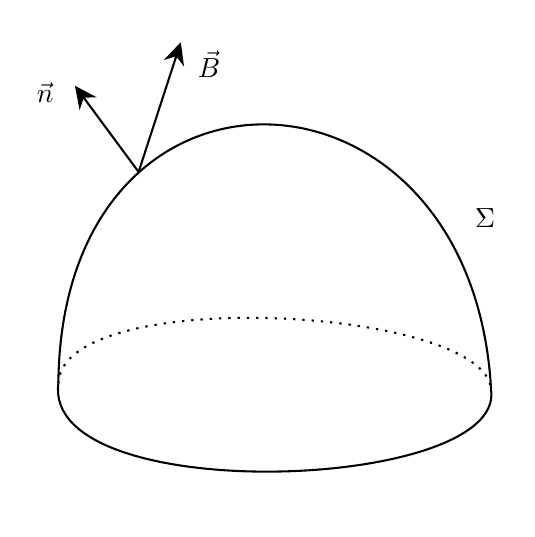
\begin{tikzpicture}[x=0.75pt,y=0.75pt,yscale=-1,xscale=1]
	%uncomment if require: \path (0,300); %set diagram left start at 0, and has height of 300

	%Curve Lines [id:da7272074769202108] 
	\draw    (209,210) .. controls (201.5,270) and (424.5,262) .. (417.5,213) ;
	%Curve Lines [id:da23093259879535255] 
	\draw  [dash pattern={on 0.84pt off 2.51pt}]  (209,210) .. controls (210.5,162) and (415.5,173) .. (417.5,213) ;
	%Curve Lines [id:da39327262602797664] 
	\draw    (209,210) .. controls (210.5,39) and (408.5,47) .. (417.5,213) ;
	%Straight Lines [id:da3821458906147317] 
	\draw    (247.67,108) -- (218.78,68.91) ;
	\draw [shift={(217,66.5)}, rotate = 413.53999999999996] [fill={rgb, 255:red, 0; green, 0; blue, 0 }  ][line width=0.08]  [draw opacity=0] (10.72,-5.15) -- (0,0) -- (10.72,5.15) -- (7.12,0) -- cycle    ;
	%Straight Lines [id:da5165175504778032] 
	\draw    (247.67,108) -- (267.07,48.35) ;
	\draw [shift={(268,45.5)}, rotate = 468.02] [fill={rgb, 255:red, 0; green, 0; blue, 0 }  ][line width=0.08]  [draw opacity=0] (10.72,-5.15) -- (0,0) -- (10.72,5.15) -- (7.12,0) -- cycle    ;

	% Text Node
	\draw (414.67,130) node    {$\Sigma $};
	% Text Node
	\draw (202.67,70) node    {$\vec{n}$};
	% Text Node
	\draw (281.67,56) node    {$\vec{B}$};

	\end{tikzpicture}
\end{figure}
\FloatBarrier

\section{Fenomeni magnetostatici nella materia}

Per parlare di questo argomento dobbiamo introdurre il solenoide rettilineo infinito, con $N_s$ numero di spire per unità di lunghezza. È un circuito in cui un filo conduttore viene avvolto su un supporto cilindrico cavo.

\begin{figure}[htpb]
	\centering

	\tikzset{every picture/.style={line width=0.75pt}} %set default line width to 0.75pt        

	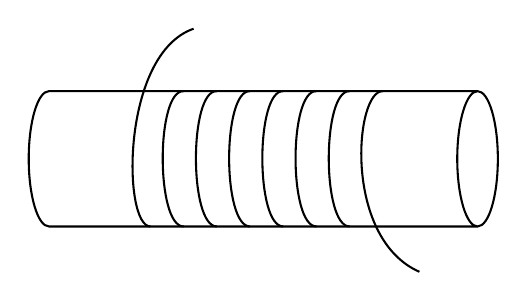
\begin{tikzpicture}[x=0.75pt,y=0.75pt,yscale=-0.8,xscale=0.8]
	%uncomment if require: \path (0,300); %set diagram left start at 0, and has height of 300

	%Shape: Can [id:dp045013765137410955] 
	\draw   (386.81,167.5) -- (128.72,167.5) .. controls (121.97,167.5) and (116.5,149.26) .. (116.5,126.75) .. controls (116.5,104.24) and (121.97,86) .. (128.72,86) -- (386.81,86) .. controls (393.56,86) and (399.03,104.24) .. (399.03,126.75) .. controls (399.03,149.26) and (393.56,167.5) .. (386.81,167.5) .. controls (380.06,167.5) and (374.58,149.26) .. (374.58,126.75) .. controls (374.58,104.24) and (380.06,86) .. (386.81,86) ;
	%Curve Lines [id:da22142605208872257] 
	\draw    (215.8,48.4) .. controls (171.8,63.6) and (173,167.6) .. (189.81,167.5) ;
	%Curve Lines [id:da21365082906938282] 
	\draw    (209.81,86) .. controls (193,85.2) and (193,167.6) .. (209.81,167.5) ;
	%Curve Lines [id:da22930047139455945] 
	\draw    (229.81,86) .. controls (213,85.2) and (213,167.6) .. (229.81,167.5) ;
	%Curve Lines [id:da7450044653523427] 
	\draw    (249.81,86) .. controls (233,85.2) and (233,167.6) .. (249.81,167.5) ;
	%Curve Lines [id:da45467405986713083] 
	\draw    (269.81,86) .. controls (253,85.2) and (253,167.6) .. (269.81,167.5) ;
	%Curve Lines [id:da9056531400522023] 
	\draw    (289.81,86) .. controls (273,85.2) and (273,167.6) .. (289.81,167.5) ;
	%Curve Lines [id:da5705660849247445] 
	\draw    (309.81,86) .. controls (293,85.2) and (293,167.6) .. (309.81,167.5) ;
	%Curve Lines [id:da46102047817662717] 
	\draw    (329.81,86) .. controls (313,85.2) and (305.4,174.4) .. (351.8,194.8) ;

	\end{tikzpicture}
\end{figure}
\FloatBarrier

Si dimostra che, se facciamo circolare nel solenoide una corrente stazionaria $I$, genereremo all'interno di esso un campo magnetico uniforme. Il verso di tale campo è determinato dalla regola del cavatappi, la direzione è quella dell'asse del solenoide. Tale campo può essere calcolato con la legge di Ampere. Se introduciamo il versore uz parallelo all'asse, possiamo scrivere questo campo come: $\vec{B}_0 = \mu_0 N_sI\vec{u}_z$.

\begin{figure}[htpb]
	\centering

	\tikzset{every picture/.style={line width=0.75pt}} %set default line width to 0.75pt        

	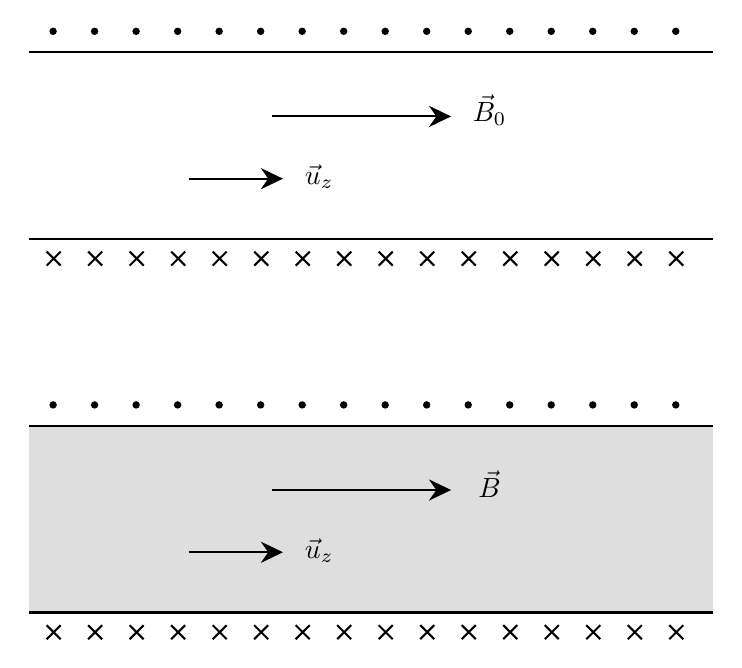
\begin{tikzpicture}[x=0.75pt,y=0.75pt,yscale=-1,xscale=1]
	%uncomment if require: \path (0,443); %set diagram left start at 0, and has height of 443

	%Shape: Rectangle [id:dp3570439802483778] 
	\draw  [draw opacity=0][fill={rgb, 255:red, 222; green, 222; blue, 222 }  ,fill opacity=1 ] (136,289) -- (465.5,289) -- (465.5,379) -- (136,379) -- cycle ;
	%Straight Lines [id:da36567456999813075] 
	\draw    (136,109) -- (465.5,109) ;
	%Shape: Circle [id:dp06167117646965958] 
	\draw  [fill={rgb, 255:red, 0; green, 0; blue, 0 }  ,fill opacity=1 ] (146.5,99) .. controls (146.5,98.31) and (147.06,97.75) .. (147.75,97.75) .. controls (148.44,97.75) and (149,98.31) .. (149,99) .. controls (149,99.69) and (148.44,100.25) .. (147.75,100.25) .. controls (147.06,100.25) and (146.5,99.69) .. (146.5,99) -- cycle ;
	%Straight Lines [id:da4511644058526041] 
	\draw    (253,140) -- (336.5,140) ;
	\draw [shift={(339.5,140)}, rotate = 180] [fill={rgb, 255:red, 0; green, 0; blue, 0 }  ][line width=0.08]  [draw opacity=0] (10.72,-5.15) -- (0,0) -- (10.72,5.15) -- (7.12,0) -- cycle    ;
	%Shape: Circle [id:dp5660420390804164] 
	\draw  [fill={rgb, 255:red, 0; green, 0; blue, 0 }  ,fill opacity=1 ] (166.5,99) .. controls (166.5,98.31) and (167.06,97.75) .. (167.75,97.75) .. controls (168.44,97.75) and (169,98.31) .. (169,99) .. controls (169,99.69) and (168.44,100.25) .. (167.75,100.25) .. controls (167.06,100.25) and (166.5,99.69) .. (166.5,99) -- cycle ;
	%Shape: Circle [id:dp07328533443252061] 
	\draw  [fill={rgb, 255:red, 0; green, 0; blue, 0 }  ,fill opacity=1 ] (186.5,99) .. controls (186.5,98.31) and (187.06,97.75) .. (187.75,97.75) .. controls (188.44,97.75) and (189,98.31) .. (189,99) .. controls (189,99.69) and (188.44,100.25) .. (187.75,100.25) .. controls (187.06,100.25) and (186.5,99.69) .. (186.5,99) -- cycle ;
	%Shape: Circle [id:dp18300326771712694] 
	\draw  [fill={rgb, 255:red, 0; green, 0; blue, 0 }  ,fill opacity=1 ] (206.5,99) .. controls (206.5,98.31) and (207.06,97.75) .. (207.75,97.75) .. controls (208.44,97.75) and (209,98.31) .. (209,99) .. controls (209,99.69) and (208.44,100.25) .. (207.75,100.25) .. controls (207.06,100.25) and (206.5,99.69) .. (206.5,99) -- cycle ;
	%Shape: Circle [id:dp608039457212683] 
	\draw  [fill={rgb, 255:red, 0; green, 0; blue, 0 }  ,fill opacity=1 ] (226.5,99) .. controls (226.5,98.31) and (227.06,97.75) .. (227.75,97.75) .. controls (228.44,97.75) and (229,98.31) .. (229,99) .. controls (229,99.69) and (228.44,100.25) .. (227.75,100.25) .. controls (227.06,100.25) and (226.5,99.69) .. (226.5,99) -- cycle ;
	%Shape: Circle [id:dp5829775483860742] 
	\draw  [fill={rgb, 255:red, 0; green, 0; blue, 0 }  ,fill opacity=1 ] (246.5,99) .. controls (246.5,98.31) and (247.06,97.75) .. (247.75,97.75) .. controls (248.44,97.75) and (249,98.31) .. (249,99) .. controls (249,99.69) and (248.44,100.25) .. (247.75,100.25) .. controls (247.06,100.25) and (246.5,99.69) .. (246.5,99) -- cycle ;
	%Shape: Circle [id:dp8365393693985355] 
	\draw  [fill={rgb, 255:red, 0; green, 0; blue, 0 }  ,fill opacity=1 ] (266.5,99) .. controls (266.5,98.31) and (267.06,97.75) .. (267.75,97.75) .. controls (268.44,97.75) and (269,98.31) .. (269,99) .. controls (269,99.69) and (268.44,100.25) .. (267.75,100.25) .. controls (267.06,100.25) and (266.5,99.69) .. (266.5,99) -- cycle ;
	%Shape: Circle [id:dp9211812805367365] 
	\draw  [fill={rgb, 255:red, 0; green, 0; blue, 0 }  ,fill opacity=1 ] (286.5,99) .. controls (286.5,98.31) and (287.06,97.75) .. (287.75,97.75) .. controls (288.44,97.75) and (289,98.31) .. (289,99) .. controls (289,99.69) and (288.44,100.25) .. (287.75,100.25) .. controls (287.06,100.25) and (286.5,99.69) .. (286.5,99) -- cycle ;
	%Shape: Circle [id:dp7579180001977182] 
	\draw  [fill={rgb, 255:red, 0; green, 0; blue, 0 }  ,fill opacity=1 ] (306.5,99) .. controls (306.5,98.31) and (307.06,97.75) .. (307.75,97.75) .. controls (308.44,97.75) and (309,98.31) .. (309,99) .. controls (309,99.69) and (308.44,100.25) .. (307.75,100.25) .. controls (307.06,100.25) and (306.5,99.69) .. (306.5,99) -- cycle ;
	%Shape: Circle [id:dp4615158289408525] 
	\draw  [fill={rgb, 255:red, 0; green, 0; blue, 0 }  ,fill opacity=1 ] (326.5,99) .. controls (326.5,98.31) and (327.06,97.75) .. (327.75,97.75) .. controls (328.44,97.75) and (329,98.31) .. (329,99) .. controls (329,99.69) and (328.44,100.25) .. (327.75,100.25) .. controls (327.06,100.25) and (326.5,99.69) .. (326.5,99) -- cycle ;
	%Shape: Circle [id:dp46502921133551056] 
	\draw  [fill={rgb, 255:red, 0; green, 0; blue, 0 }  ,fill opacity=1 ] (346.5,99) .. controls (346.5,98.31) and (347.06,97.75) .. (347.75,97.75) .. controls (348.44,97.75) and (349,98.31) .. (349,99) .. controls (349,99.69) and (348.44,100.25) .. (347.75,100.25) .. controls (347.06,100.25) and (346.5,99.69) .. (346.5,99) -- cycle ;
	%Shape: Circle [id:dp6969228625535551] 
	\draw  [fill={rgb, 255:red, 0; green, 0; blue, 0 }  ,fill opacity=1 ] (366.5,99) .. controls (366.5,98.31) and (367.06,97.75) .. (367.75,97.75) .. controls (368.44,97.75) and (369,98.31) .. (369,99) .. controls (369,99.69) and (368.44,100.25) .. (367.75,100.25) .. controls (367.06,100.25) and (366.5,99.69) .. (366.5,99) -- cycle ;
	%Shape: Circle [id:dp7115874827419801] 
	\draw  [fill={rgb, 255:red, 0; green, 0; blue, 0 }  ,fill opacity=1 ] (386.5,99) .. controls (386.5,98.31) and (387.06,97.75) .. (387.75,97.75) .. controls (388.44,97.75) and (389,98.31) .. (389,99) .. controls (389,99.69) and (388.44,100.25) .. (387.75,100.25) .. controls (387.06,100.25) and (386.5,99.69) .. (386.5,99) -- cycle ;
	%Shape: Circle [id:dp9086685091559468] 
	\draw  [fill={rgb, 255:red, 0; green, 0; blue, 0 }  ,fill opacity=1 ] (406.5,99) .. controls (406.5,98.31) and (407.06,97.75) .. (407.75,97.75) .. controls (408.44,97.75) and (409,98.31) .. (409,99) .. controls (409,99.69) and (408.44,100.25) .. (407.75,100.25) .. controls (407.06,100.25) and (406.5,99.69) .. (406.5,99) -- cycle ;
	%Shape: Circle [id:dp026018660569895546] 
	\draw  [fill={rgb, 255:red, 0; green, 0; blue, 0 }  ,fill opacity=1 ] (426.5,99) .. controls (426.5,98.31) and (427.06,97.75) .. (427.75,97.75) .. controls (428.44,97.75) and (429,98.31) .. (429,99) .. controls (429,99.69) and (428.44,100.25) .. (427.75,100.25) .. controls (427.06,100.25) and (426.5,99.69) .. (426.5,99) -- cycle ;
	%Shape: Circle [id:dp4647458311205046] 
	\draw  [fill={rgb, 255:red, 0; green, 0; blue, 0 }  ,fill opacity=1 ] (446.5,99) .. controls (446.5,98.31) and (447.06,97.75) .. (447.75,97.75) .. controls (448.44,97.75) and (449,98.31) .. (449,99) .. controls (449,99.69) and (448.44,100.25) .. (447.75,100.25) .. controls (447.06,100.25) and (446.5,99.69) .. (446.5,99) -- cycle ;
	\draw   (144.63,205.13) -- (151.38,211.88)(151.38,205.13) -- (144.63,211.88) ;
	\draw   (164.63,205.13) -- (171.38,211.88)(171.38,205.13) -- (164.63,211.88) ;
	\draw   (184.63,205.13) -- (191.38,211.88)(191.38,205.13) -- (184.63,211.88) ;
	\draw   (204.63,205.13) -- (211.38,211.88)(211.38,205.13) -- (204.63,211.88) ;
	\draw   (224.63,205.13) -- (231.38,211.88)(231.38,205.13) -- (224.63,211.88) ;
	\draw   (244.63,205.13) -- (251.38,211.88)(251.38,205.13) -- (244.63,211.88) ;
	\draw   (264.63,205.13) -- (271.38,211.88)(271.38,205.13) -- (264.63,211.88) ;
	\draw   (284.63,205.13) -- (291.38,211.88)(291.38,205.13) -- (284.63,211.88) ;
	\draw   (304.63,205.13) -- (311.38,211.88)(311.38,205.13) -- (304.63,211.88) ;
	\draw   (324.63,205.13) -- (331.38,211.88)(331.38,205.13) -- (324.63,211.88) ;
	\draw   (344.63,205.13) -- (351.38,211.88)(351.38,205.13) -- (344.63,211.88) ;
	\draw   (364.63,205.13) -- (371.38,211.88)(371.38,205.13) -- (364.63,211.88) ;
	\draw   (384.63,205.13) -- (391.38,211.88)(391.38,205.13) -- (384.63,211.88) ;
	\draw   (404.63,205.13) -- (411.38,211.88)(411.38,205.13) -- (404.63,211.88) ;
	\draw   (424.63,205.13) -- (431.38,211.88)(431.38,205.13) -- (424.63,211.88) ;
	\draw   (444.63,205.13) -- (451.38,211.88)(451.38,205.13) -- (444.63,211.88) ;
	%Straight Lines [id:da011930091129263687] 
	\draw    (136,199) -- (465.5,199) ;
	%Straight Lines [id:da8541905804450896] 
	\draw    (213,170) -- (255.5,170) ;
	\draw [shift={(258.5,170)}, rotate = 180] [fill={rgb, 255:red, 0; green, 0; blue, 0 }  ][line width=0.08]  [draw opacity=0] (10.72,-5.15) -- (0,0) -- (10.72,5.15) -- (7.12,0) -- cycle    ;
	%Straight Lines [id:da5131266363848697] 
	\draw    (136,289) -- (465.5,289) ;
	%Shape: Circle [id:dp7651147863040559] 
	\draw  [fill={rgb, 255:red, 0; green, 0; blue, 0 }  ,fill opacity=1 ] (146.5,279) .. controls (146.5,278.31) and (147.06,277.75) .. (147.75,277.75) .. controls (148.44,277.75) and (149,278.31) .. (149,279) .. controls (149,279.69) and (148.44,280.25) .. (147.75,280.25) .. controls (147.06,280.25) and (146.5,279.69) .. (146.5,279) -- cycle ;
	%Straight Lines [id:da4325803733652427] 
	\draw    (253,320) -- (336.5,320) ;
	\draw [shift={(339.5,320)}, rotate = 180] [fill={rgb, 255:red, 0; green, 0; blue, 0 }  ][line width=0.08]  [draw opacity=0] (10.72,-5.15) -- (0,0) -- (10.72,5.15) -- (7.12,0) -- cycle    ;
	%Shape: Circle [id:dp4114711006213514] 
	\draw  [fill={rgb, 255:red, 0; green, 0; blue, 0 }  ,fill opacity=1 ] (166.5,279) .. controls (166.5,278.31) and (167.06,277.75) .. (167.75,277.75) .. controls (168.44,277.75) and (169,278.31) .. (169,279) .. controls (169,279.69) and (168.44,280.25) .. (167.75,280.25) .. controls (167.06,280.25) and (166.5,279.69) .. (166.5,279) -- cycle ;
	%Shape: Circle [id:dp6622056757528201] 
	\draw  [fill={rgb, 255:red, 0; green, 0; blue, 0 }  ,fill opacity=1 ] (186.5,279) .. controls (186.5,278.31) and (187.06,277.75) .. (187.75,277.75) .. controls (188.44,277.75) and (189,278.31) .. (189,279) .. controls (189,279.69) and (188.44,280.25) .. (187.75,280.25) .. controls (187.06,280.25) and (186.5,279.69) .. (186.5,279) -- cycle ;
	%Shape: Circle [id:dp08439361314545968] 
	\draw  [fill={rgb, 255:red, 0; green, 0; blue, 0 }  ,fill opacity=1 ] (206.5,279) .. controls (206.5,278.31) and (207.06,277.75) .. (207.75,277.75) .. controls (208.44,277.75) and (209,278.31) .. (209,279) .. controls (209,279.69) and (208.44,280.25) .. (207.75,280.25) .. controls (207.06,280.25) and (206.5,279.69) .. (206.5,279) -- cycle ;
	%Shape: Circle [id:dp208931867674091] 
	\draw  [fill={rgb, 255:red, 0; green, 0; blue, 0 }  ,fill opacity=1 ] (226.5,279) .. controls (226.5,278.31) and (227.06,277.75) .. (227.75,277.75) .. controls (228.44,277.75) and (229,278.31) .. (229,279) .. controls (229,279.69) and (228.44,280.25) .. (227.75,280.25) .. controls (227.06,280.25) and (226.5,279.69) .. (226.5,279) -- cycle ;
	%Shape: Circle [id:dp24176455894853666] 
	\draw  [fill={rgb, 255:red, 0; green, 0; blue, 0 }  ,fill opacity=1 ] (246.5,279) .. controls (246.5,278.31) and (247.06,277.75) .. (247.75,277.75) .. controls (248.44,277.75) and (249,278.31) .. (249,279) .. controls (249,279.69) and (248.44,280.25) .. (247.75,280.25) .. controls (247.06,280.25) and (246.5,279.69) .. (246.5,279) -- cycle ;
	%Shape: Circle [id:dp7134986809671351] 
	\draw  [fill={rgb, 255:red, 0; green, 0; blue, 0 }  ,fill opacity=1 ] (266.5,279) .. controls (266.5,278.31) and (267.06,277.75) .. (267.75,277.75) .. controls (268.44,277.75) and (269,278.31) .. (269,279) .. controls (269,279.69) and (268.44,280.25) .. (267.75,280.25) .. controls (267.06,280.25) and (266.5,279.69) .. (266.5,279) -- cycle ;
	%Shape: Circle [id:dp4301034087995177] 
	\draw  [fill={rgb, 255:red, 0; green, 0; blue, 0 }  ,fill opacity=1 ] (286.5,279) .. controls (286.5,278.31) and (287.06,277.75) .. (287.75,277.75) .. controls (288.44,277.75) and (289,278.31) .. (289,279) .. controls (289,279.69) and (288.44,280.25) .. (287.75,280.25) .. controls (287.06,280.25) and (286.5,279.69) .. (286.5,279) -- cycle ;
	%Shape: Circle [id:dp3141736429267601] 
	\draw  [fill={rgb, 255:red, 0; green, 0; blue, 0 }  ,fill opacity=1 ] (306.5,279) .. controls (306.5,278.31) and (307.06,277.75) .. (307.75,277.75) .. controls (308.44,277.75) and (309,278.31) .. (309,279) .. controls (309,279.69) and (308.44,280.25) .. (307.75,280.25) .. controls (307.06,280.25) and (306.5,279.69) .. (306.5,279) -- cycle ;
	%Shape: Circle [id:dp7904314939792563] 
	\draw  [fill={rgb, 255:red, 0; green, 0; blue, 0 }  ,fill opacity=1 ] (326.5,279) .. controls (326.5,278.31) and (327.06,277.75) .. (327.75,277.75) .. controls (328.44,277.75) and (329,278.31) .. (329,279) .. controls (329,279.69) and (328.44,280.25) .. (327.75,280.25) .. controls (327.06,280.25) and (326.5,279.69) .. (326.5,279) -- cycle ;
	%Shape: Circle [id:dp8568388528321926] 
	\draw  [fill={rgb, 255:red, 0; green, 0; blue, 0 }  ,fill opacity=1 ] (346.5,279) .. controls (346.5,278.31) and (347.06,277.75) .. (347.75,277.75) .. controls (348.44,277.75) and (349,278.31) .. (349,279) .. controls (349,279.69) and (348.44,280.25) .. (347.75,280.25) .. controls (347.06,280.25) and (346.5,279.69) .. (346.5,279) -- cycle ;
	%Shape: Circle [id:dp4917928487527021] 
	\draw  [fill={rgb, 255:red, 0; green, 0; blue, 0 }  ,fill opacity=1 ] (366.5,279) .. controls (366.5,278.31) and (367.06,277.75) .. (367.75,277.75) .. controls (368.44,277.75) and (369,278.31) .. (369,279) .. controls (369,279.69) and (368.44,280.25) .. (367.75,280.25) .. controls (367.06,280.25) and (366.5,279.69) .. (366.5,279) -- cycle ;
	%Shape: Circle [id:dp35777580605743875] 
	\draw  [fill={rgb, 255:red, 0; green, 0; blue, 0 }  ,fill opacity=1 ] (386.5,279) .. controls (386.5,278.31) and (387.06,277.75) .. (387.75,277.75) .. controls (388.44,277.75) and (389,278.31) .. (389,279) .. controls (389,279.69) and (388.44,280.25) .. (387.75,280.25) .. controls (387.06,280.25) and (386.5,279.69) .. (386.5,279) -- cycle ;
	%Shape: Circle [id:dp4453998005278139] 
	\draw  [fill={rgb, 255:red, 0; green, 0; blue, 0 }  ,fill opacity=1 ] (406.5,279) .. controls (406.5,278.31) and (407.06,277.75) .. (407.75,277.75) .. controls (408.44,277.75) and (409,278.31) .. (409,279) .. controls (409,279.69) and (408.44,280.25) .. (407.75,280.25) .. controls (407.06,280.25) and (406.5,279.69) .. (406.5,279) -- cycle ;
	%Shape: Circle [id:dp6724734928969023] 
	\draw  [fill={rgb, 255:red, 0; green, 0; blue, 0 }  ,fill opacity=1 ] (426.5,279) .. controls (426.5,278.31) and (427.06,277.75) .. (427.75,277.75) .. controls (428.44,277.75) and (429,278.31) .. (429,279) .. controls (429,279.69) and (428.44,280.25) .. (427.75,280.25) .. controls (427.06,280.25) and (426.5,279.69) .. (426.5,279) -- cycle ;
	%Shape: Circle [id:dp16204380586234945] 
	\draw  [fill={rgb, 255:red, 0; green, 0; blue, 0 }  ,fill opacity=1 ] (446.5,279) .. controls (446.5,278.31) and (447.06,277.75) .. (447.75,277.75) .. controls (448.44,277.75) and (449,278.31) .. (449,279) .. controls (449,279.69) and (448.44,280.25) .. (447.75,280.25) .. controls (447.06,280.25) and (446.5,279.69) .. (446.5,279) -- cycle ;
	\draw   (144.63,385.13) -- (151.38,391.88)(151.38,385.13) -- (144.63,391.88) ;
	\draw   (164.63,385.13) -- (171.38,391.88)(171.38,385.13) -- (164.63,391.88) ;
	\draw   (184.63,385.13) -- (191.38,391.88)(191.38,385.13) -- (184.63,391.88) ;
	\draw   (204.63,385.13) -- (211.38,391.88)(211.38,385.13) -- (204.63,391.88) ;
	\draw   (224.63,385.13) -- (231.38,391.88)(231.38,385.13) -- (224.63,391.88) ;
	\draw   (244.63,385.13) -- (251.38,391.88)(251.38,385.13) -- (244.63,391.88) ;
	\draw   (264.63,385.13) -- (271.38,391.88)(271.38,385.13) -- (264.63,391.88) ;
	\draw   (284.63,385.13) -- (291.38,391.88)(291.38,385.13) -- (284.63,391.88) ;
	\draw   (304.63,385.13) -- (311.38,391.88)(311.38,385.13) -- (304.63,391.88) ;
	\draw   (324.63,385.13) -- (331.38,391.88)(331.38,385.13) -- (324.63,391.88) ;
	\draw   (344.63,385.13) -- (351.38,391.88)(351.38,385.13) -- (344.63,391.88) ;
	\draw   (364.63,385.13) -- (371.38,391.88)(371.38,385.13) -- (364.63,391.88) ;
	\draw   (384.63,385.13) -- (391.38,391.88)(391.38,385.13) -- (384.63,391.88) ;
	\draw   (404.63,385.13) -- (411.38,391.88)(411.38,385.13) -- (404.63,391.88) ;
	\draw   (424.63,385.13) -- (431.38,391.88)(431.38,385.13) -- (424.63,391.88) ;
	\draw   (444.63,385.13) -- (451.38,391.88)(451.38,385.13) -- (444.63,391.88) ;
	%Straight Lines [id:da6433239934847432] 
	\draw    (136,379) -- (465.5,379) ;
	%Straight Lines [id:da1810416487609825] 
	\draw    (213,350) -- (255.5,350) ;
	\draw [shift={(258.5,350)}, rotate = 180] [fill={rgb, 255:red, 0; green, 0; blue, 0 }  ][line width=0.08]  [draw opacity=0] (10.72,-5.15) -- (0,0) -- (10.72,5.15) -- (7.12,0) -- cycle    ;

	% Text Node
	\draw (358,137) node    {$\vec{B}_{0}$};
	% Text Node
	\draw (276,169) node    {$\vec{u}_{z}$};
	% Text Node
	\draw (358,317) node    {$\vec{B}$};
	% Text Node
	\draw (276,349) node    {$\vec{u}_{z}$};

	\end{tikzpicture}
\end{figure}
\FloatBarrier

Se, a parità di corrente, inseriamo all'interno del solenoide un materiale avremo $ \vec{B}  \neq \vec{B}_0  $. Definiamo allora

\begin{gather*}
	\frac{B}{B_0}= \mu_r \qquad \text{permeabilità magnetica relativa del materiale} \\
	\mu = \mu_0 \mu_r \qquad \text{permeabilità magnetica assoluta del materiale}
\end{gather*}

Infine

\[
	\chi_m = \mu_r -1 \qquad \text{suscettività magnetica relativa del materiale}
\]

Possiamo quindi dire

\[
	\vec{B} = \mu_r \vec{B}_0 = (1 + \chi_m) \vec{B}_0 = \vec{B}_0 + \chi_m\vec{B}_0
\]

Il secondo termine rappresenta l'effetto del mezzo magnetizzato, che risulta identico a quello che sarebbe prodotto da un secondo solenoide eguale al primo, ma percorso da una corrente di densità lineare differente. Questa interpretazione non è fittizia: sulla superficie del mezzo magnetizzato esiste veramente una corrente, risultato di correnti di origine atomica che si formano per effetto del campo magnetico prodotto dalla corrente di conduzione. Tale correnti sono dette amperiane.
Il vuoto stesso può essere consderato un mezzo particolare di permeabilità magnetica relativa $ \mu_r = 1 $.

Sperimentalmente, a questo punto ci si presentano 3 casi.

\begin{itemize}
	\item \textbf{Materiali diamagnetici} (es. argento, oro, rame, elio, $\dots$) \\
	In questo caso si ha che $\boxed{ \mu_r < 1 \implies \chi_m < 0}$\\
	$ \chi_m  $ risulta indipendente dalla temperatura e ha valori compresi tra $ -10^{-5} < \chi_m < -10^{-9} $

	\item \textbf{Materiali paramagnetici} (es. alluminio, cromo, ossigeno, $\dots$) \\
	In questo caso si ha che $\boxed{ \mu_r > 1 \implies \chi_m > 0} $\\
	$ \chi_m  $ dipende dalla temperatura $ \left( \chi_m=\frac{c\rho}{T} \right)   $ (\emph{legge di Curie})  e ha valori compresi tra \\ $10^{-6}<\chi_m<10^{-2}$

	\item \textbf{Materiali ferromagnetici}\\
	In questo caso si ha che $\boxed{ \mu_r \sim [10^2\ldots 10^5]}$\\
	$ \chi_m  $ dipende dalla temperatura $ \left( \chi_m=\frac{c\rho}{T-T_c} \right) $ (\emph{legge di Curie-Weiss})\\
	Per temperature $ T>T_c $ (temperatura di Curie), i materiali ferromagnetici diventano paramagnetici.
\end{itemize}

In analogia con le cariche di polarizzazione viste per il campo elettrico, il fatto che $ \vec{B} \neq \vec{B}_0  $ si può ricondurre a delle \textbf{correnti di magnetizzazione superficiali}, dette anche correnti \emph{correnti amperiane}.

\section{Correnti di magnetizzazione superficiali (o correnti amperiane)}

Abbiamo visto che si può dimostrare che in un materiale omogeneo isotropo esposto a un campo magnetico compaiono correnti sulla sua superficie che generano un campo magnetico che va a sommarsi a $ \vec{B}_0  $.

Consideriamo un atomo di quelli che compongono il materiale e schematizziamolo come una carica positiva attorno alla quale orbita un elettrone. L'oggetto può essere visto come un circuito microscopico percorso da corrente. Il verso della corrente equivalente è opposto rispetto alla velocità dell'elettrone. Tale circuito genera a sua volta un momento di dipolo magnetico se immerso in un campo $\vec{B}$ e si comporta come un dipolo elettrico immerso in un campo $\vec{E}$.

L'atomo può essere visto come una spira piana di area $ \pi r^2  $
Percorsa dalla corrente $ i_a  $ (verso opposto alla velocità dell'elettrone), la quale equivale, agli effetti magnetici, per il principio di equivalenza di Ampere, a un dipolo elementare di momento magnetico:

\[
	\vec{m} =IS\vec{n} = I\pi r^2 \vec{n}
\]

\begin{figure}[htpb]
	\centering

	\tikzset{every picture/.style={line width=0.75pt}} %set default line width to 0.75pt        

	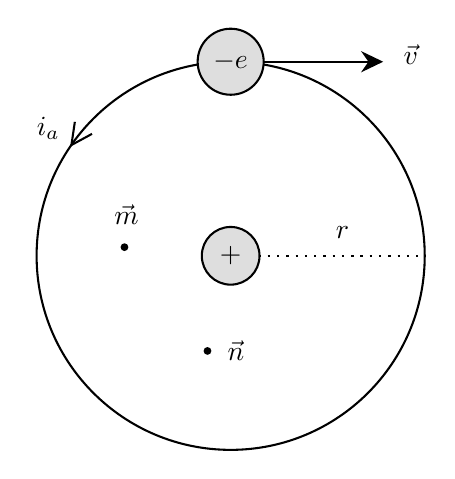
\begin{tikzpicture}[x=0.75pt,y=0.75pt,yscale=-1,xscale=1]
	%uncomment if require: \path (0,300); %set diagram left start at 0, and has height of 300

	%Shape: Circle [id:dp2712735899479499] 
	\draw   (189,166.5) .. controls (189,114.86) and (230.86,73) .. (282.5,73) .. controls (334.14,73) and (376,114.86) .. (376,166.5) .. controls (376,218.14) and (334.14,260) .. (282.5,260) .. controls (230.86,260) and (189,218.14) .. (189,166.5) -- cycle ;
	%Straight Lines [id:da6534809017110852] 
	\draw    (282.5,73) -- (353,73) ;
	\draw [shift={(356,73)}, rotate = 180] [fill={rgb, 255:red, 0; green, 0; blue, 0 }  ][line width=0.08]  [draw opacity=0] (10.72,-5.15) -- (0,0) -- (10.72,5.15) -- (7.12,0) -- cycle    ;
	\draw   (215.7,107.76) -- (205.77,113.14) -- (207.43,101.96) ;
	%Straight Lines [id:da03521882584841718] 
	\draw  [dash pattern={on 0.84pt off 2.51pt}]  (282.5,166.5) -- (376,166.5) ;
	%Shape: Circle [id:dp8491457574334582] 
	\draw  [fill={rgb, 255:red, 0; green, 0; blue, 0 }  ,fill opacity=1 ] (230,162.33) .. controls (230,161.6) and (230.6,161) .. (231.33,161) .. controls (232.07,161) and (232.67,161.6) .. (232.67,162.33) .. controls (232.67,163.07) and (232.07,163.67) .. (231.33,163.67) .. controls (230.6,163.67) and (230,163.07) .. (230,162.33) -- cycle ;
	%Shape: Circle [id:dp8737946612729182] 
	\draw  [fill={rgb, 255:red, 0; green, 0; blue, 0 }  ,fill opacity=1 ] (270,212.33) .. controls (270,211.6) and (270.6,211) .. (271.33,211) .. controls (272.07,211) and (272.67,211.6) .. (272.67,212.33) .. controls (272.67,213.07) and (272.07,213.67) .. (271.33,213.67) .. controls (270.6,213.67) and (270,213.07) .. (270,212.33) -- cycle ;

	% Text Node
	\draw  [fill={rgb, 255:red, 222; green, 222; blue, 222 }  ,fill opacity=1 ]  (282.5, 73) circle [x radius= 15.91, y radius= 15.91]   ;
	\draw (282.5,73) node    {$-e$};
	% Text Node
	\draw (194.67,105) node    {$i_{a}$};
	% Text Node
	\draw  [fill={rgb, 255:red, 222; green, 222; blue, 222 }  ,fill opacity=1 ]  (282.5, 166.5) circle [x radius= 13.9, y radius= 13.9]   ;
	\draw (282.5,166.5) node    {$+$};
	% Text Node
	\draw (336.33,155.33) node    {$r$};
	% Text Node
	\draw (285,212) node    {$\vec{n}$};
	% Text Node
	\draw (232.33,146.67) node    {$\vec{m}$};
	% Text Node
	\draw (369.33,69.67) node    {$\vec{v}$};

	\end{tikzpicture}
\end{figure}
\FloatBarrier

Inoltre anche gli elettroni possiedono un momento di dipolo magnetico proprio, di spin, che si somma a quello orbitale. In realtà per studiare come si sommano vettorialmente i momenti di dipolo bisognerebbe passare al modello quantistico (non classico come questo).

Si parla di magnetizzazione in presenza di un momento di dipolo magnetico macroscopico nel materiale.
Esistono due meccanismi di magnetizzazione:

\begin{itemize}
	\item \textbf{Precessione di Larmor.} Dobbiamo distinguere fra campo magnetico totale macroscopico e campo magnetico locale. Quest'ultimo non comprende infatti il contributo del singolo atomo. Il moto degli elettroni intorno al nucleo può essere assimilato a correnti microscopiche, alle quali è associato un momento magnetico. Nella maggior parte dei casi questi momenti si compensano e l'atomo non ha momento magnetico, mentre quando agisce un campo magnetico esterno il moto degli elettroni è perturbato e ha origine un momento magnetico (di Larmor) che è opposto al campo esterno: questo è il meccanismo classico del diamagnetismo.
	\item \textbf{Magnetizzazione per orientamento.} In alcune sostanze vi sono condizioni di asimmetria per cui le molecole possono avere un momento magnetico intrinseco. In assenza di campo esterno c'è una distribuzione casuale dei momenti di dipolo. In assenza di perturbazione, a causa dell'agitazione termica si ha:
	\[
		\langle\vec{m} \rangle=0
	\]
	Sotto l'azione magnetica c'è un fenomeno di orientazione parziale e ha origine un momento magnetico parallelo e concorde al campo esterno, che supera l'effetto diamagnetico. Questo è ciò che accade nei materiali paramagnetici.
	\begin{figure}[htpb]
		\centering
		

		\tikzset{every picture/.style={line width=0.75pt}} %set default line width to 0.75pt        

		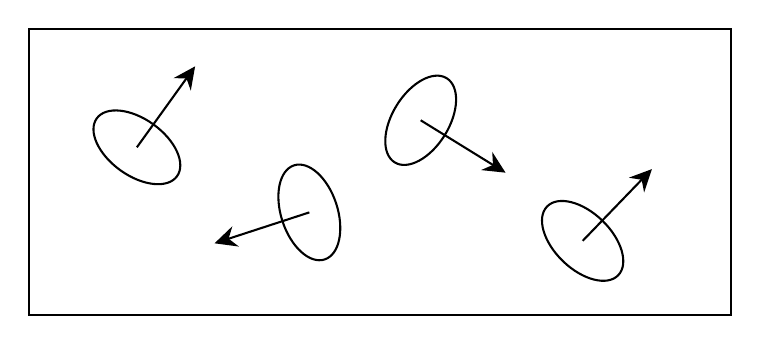
\begin{tikzpicture}[x=0.75pt,y=0.75pt,yscale=-1,xscale=1]
		%uncomment if require: \path (0,300); %set diagram left start at 0, and has height of 300

		%Shape: Rectangle [id:dp501883048787948] 
		\draw   (127,73) -- (465.5,73) -- (465.5,211) -- (127,211) -- cycle ;
		%Straight Lines [id:da5698452711857578] 
		\draw    (179.11,130.14) -- (205.42,93.57) ;
		\draw [shift={(207.17,91.14)}, rotate = 485.73] [fill={rgb, 255:red, 0; green, 0; blue, 0 }  ][line width=0.08]  [draw opacity=0] (10.72,-5.15) -- (0,0) -- (10.72,5.15) -- (7.12,0) -- cycle    ;
		%Shape: Ellipse [id:dp16811796547817082] 
		\draw   (159.77,116.22) .. controls (164.16,110.12) and (176.38,111.4) .. (187.07,119.09) .. controls (197.75,126.77) and (202.85,137.95) .. (198.46,144.06) .. controls (194.07,150.16) and (181.85,148.88) .. (171.16,141.2) .. controls (160.48,133.51) and (155.37,122.33) .. (159.77,116.22) -- cycle ;

		%Straight Lines [id:da5185904290633843] 
		\draw    (262.2,161.5) -- (219.37,175.46) ;
		\draw [shift={(216.52,176.39)}, rotate = 341.94] [fill={rgb, 255:red, 0; green, 0; blue, 0 }  ][line width=0.08]  [draw opacity=0] (10.72,-5.15) -- (0,0) -- (10.72,5.15) -- (7.12,0) -- cycle    ;
		%Shape: Ellipse [id:dp6467364427859881] 
		\draw   (269.59,184.16) .. controls (262.44,186.49) and (253.33,178.23) .. (249.25,165.72) .. controls (245.17,153.2) and (247.66,141.17) .. (254.81,138.84) .. controls (261.96,136.51) and (271.07,144.76) .. (275.15,157.27) .. controls (279.23,169.79) and (276.74,181.82) .. (269.59,184.16) -- cycle ;

		%Straight Lines [id:da304296926921781] 
		\draw    (315.85,117.12) -- (354.18,140.79) ;
		\draw [shift={(356.74,142.36)}, rotate = 211.69] [fill={rgb, 255:red, 0; green, 0; blue, 0 }  ][line width=0.08]  [draw opacity=0] (10.72,-5.15) -- (0,0) -- (10.72,5.15) -- (7.12,0) -- cycle    ;
		%Shape: Ellipse [id:dp658133593462523] 
		\draw   (328.37,96.84) .. controls (334.77,100.8) and (334.36,113.08) .. (327.44,124.28) .. controls (320.53,135.48) and (309.73,141.35) .. (303.33,137.4) .. controls (296.93,133.45) and (297.35,121.17) .. (304.26,109.97) .. controls (311.18,98.77) and (321.97,92.89) .. (328.37,96.84) -- cycle ;

		%Straight Lines [id:da9060060516988924] 
		\draw    (393.88,175.22) -- (425.16,142.81) ;
		\draw [shift={(427.25,140.65)}, rotate = 493.99] [fill={rgb, 255:red, 0; green, 0; blue, 0 }  ][line width=0.08]  [draw opacity=0] (10.72,-5.15) -- (0,0) -- (10.72,5.15) -- (7.12,0) -- cycle    ;
		%Shape: Ellipse [id:dp3999948978632739] 
		\draw   (376.73,158.67) .. controls (381.95,153.25) and (393.87,156.28) .. (403.34,165.42) .. controls (412.81,174.56) and (416.25,186.36) .. (411.02,191.77) .. controls (405.8,197.18) and (393.89,194.16) .. (384.42,185.02) .. controls (374.95,175.87) and (371.51,164.08) .. (376.73,158.67) -- cycle ;

		\end{tikzpicture}
	\end{figure}
	\FloatBarrier

	Tale orientamento è disturbato dalle collisioni quindi ci sarà equilibrio fra tendenza ad orientamento e tendenza a distribuzione casuale. Possiamo allora introdurre un momento magnetico medio come
	\[
		\vec{m}_L = -\alpha_L\vec{B}_L
	\]
	Qui $ \alpha  $ dipende dalla temperatura perché più essa aumenta più aumentano le collisioni. Tale dipendenza non c'era nel processo di Larmor perché si tratta di un processo che avviene nell'atomo.
	\[
		\langle \vec{m} \rangle = \alpha_0 \vec{B}_L \qquad \alpha_0\sim \frac{m_0^2}{3k_0T}
	\]
\end{itemize}

Consideriamo nel nostro materiale un punto e un volumetto $ \Delta \tau  $ e supponiamo che la somma di tutti i momenti magnetici all'interno del cubo sia un vettore $ \Delta \vec{m}  $. Definiamo vettore magnetizzazione nel punto $P$ il vettore:

\begin{gather*}
	\boxed{\vec{M} (P)=\lim_{\Delta \tau \to 0} \frac{\Delta \vec{m}}{\Delta \tau}} \\
	[M]=\frac{[I][L^2 ]}{[L^3 ]} = \frac{I}{L} \qquad \left( \frac{A}{m} \right)
\end{gather*}

Questa grandezza $A/m$ l'abbiamo già introdotta quando abbiamo parlato di correnti superficiali.
Consideriamo il caso di un cilindro di materiale uniformemente magnetizzato. Il vettore $\vec{M}$ in tutti i punti è costante in modulo, direzione e verso.

\begin{figure}[htpb]
	\centering

	\tikzset{every picture/.style={line width=0.75pt}} %set default line width to 0.75pt        

	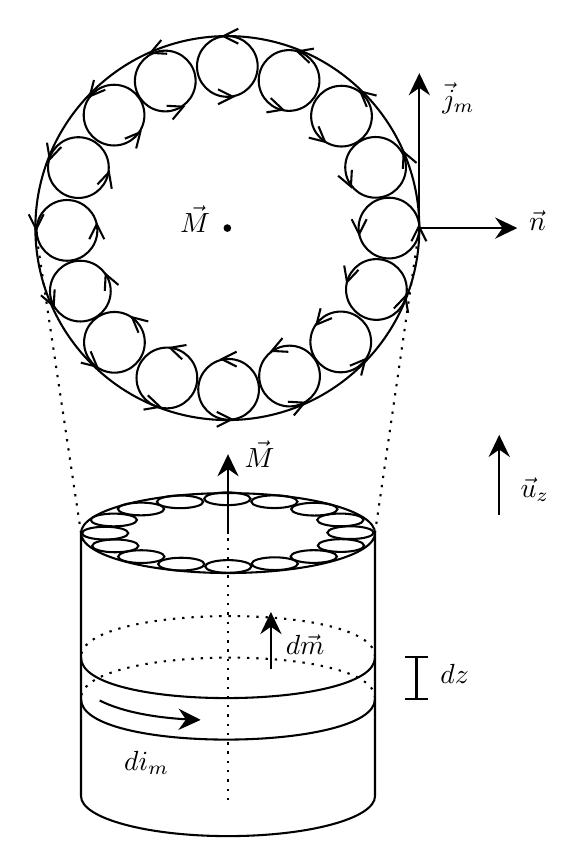
\begin{tikzpicture}[x=0.75pt,y=0.75pt,yscale=-1,xscale=1]
	%uncomment if require: \path (0,486); %set diagram left start at 0, and has height of 486

	%Shape: Can [id:dp3230615374202459] 
	\draw   (285.64,247) -- (285.64,373.75) .. controls (285.64,384.38) and (253.94,393) .. (214.82,393) .. controls (175.71,393) and (144,384.38) .. (144,373.75) -- (144,247) .. controls (144,236.37) and (175.71,227.75) .. (214.82,227.75) .. controls (253.94,227.75) and (285.64,236.37) .. (285.64,247) .. controls (285.64,257.63) and (253.94,266.24) .. (214.82,266.24) .. controls (175.71,266.24) and (144,257.63) .. (144,247) ;
	%Straight Lines [id:da17259453016301607] 
	\draw  [dash pattern={on 0.84pt off 2.51pt}]  (144,247) -- (122,100.05) ;
	%Curve Lines [id:da4364396764680176] 
	\draw    (144,327) .. controls (144,353.33) and (285.33,352.67) .. (285.64,327) ;
	%Curve Lines [id:da04570346435057404] 
	\draw    (144,307) .. controls (144,333.33) and (285.33,332.67) .. (285.64,307) ;
	%Curve Lines [id:da5518993535514329] 
	\draw  [dash pattern={on 0.84pt off 2.51pt}]  (285.64,306.5) .. controls (285.64,280.16) and (144.31,280.83) .. (144,306.5) ;
	%Curve Lines [id:da40078306322834467] 
	\draw  [dash pattern={on 0.84pt off 2.51pt}]  (285.64,326.5) .. controls (285.64,300.16) and (144.31,300.83) .. (144,326.5) ;
	%Shape: Ellipse [id:dp7888143418444162] 
	\draw   (122,100.05) .. controls (122,48.97) and (163.41,7.55) .. (214.5,7.55) .. controls (265.59,7.55) and (307,48.97) .. (307,100.05) .. controls (307,151.14) and (265.59,192.55) .. (214.5,192.55) .. controls (163.41,192.55) and (122,151.14) .. (122,100.05) -- cycle ;
	%Shape: Ellipse [id:dp8462081397971879] 
	\draw   (199.87,22.18) .. controls (199.87,14.1) and (206.42,7.55) .. (214.5,7.55) .. controls (222.58,7.55) and (229.13,14.1) .. (229.13,22.18) .. controls (229.13,30.26) and (222.58,36.81) .. (214.5,36.81) .. controls (206.42,36.81) and (199.87,30.26) .. (199.87,22.18) -- cycle ;
	%Shape: Ellipse [id:dp6804585921218491] 
	\draw   (277.74,100.05) .. controls (277.74,91.97) and (284.29,85.42) .. (292.37,85.42) .. controls (300.45,85.42) and (307,91.97) .. (307,100.05) .. controls (307,108.13) and (300.45,114.68) .. (292.37,114.68) .. controls (284.29,114.68) and (277.74,108.13) .. (277.74,100.05) -- cycle ;
	%Shape: Ellipse [id:dp7704312400046178] 
	\draw   (271.3,70.8) .. controls (271.3,62.72) and (277.85,56.17) .. (285.93,56.17) .. controls (294.01,56.17) and (300.56,62.72) .. (300.56,70.8) .. controls (300.56,78.88) and (294.01,85.42) .. (285.93,85.42) .. controls (277.85,85.42) and (271.3,78.88) .. (271.3,70.8) -- cycle ;
	%Shape: Ellipse [id:dp6850228040411508] 
	\draw   (254.87,46.12) .. controls (254.87,38.04) and (261.42,31.49) .. (269.5,31.49) .. controls (277.58,31.49) and (284.13,38.04) .. (284.13,46.12) .. controls (284.13,54.2) and (277.58,60.75) .. (269.5,60.75) .. controls (261.42,60.75) and (254.87,54.2) .. (254.87,46.12) -- cycle ;
	%Shape: Ellipse [id:dp12566774187130147] 
	\draw   (229.61,28.94) .. controls (229.61,20.86) and (236.16,14.31) .. (244.23,14.31) .. controls (252.31,14.31) and (258.86,20.86) .. (258.86,28.94) .. controls (258.86,37.02) and (252.31,43.57) .. (244.23,43.57) .. controls (236.16,43.57) and (229.61,37.02) .. (229.61,28.94) -- cycle ;
	%Shape: Ellipse [id:dp40074758889659146] 
	\draw   (229.74,177.75) .. controls (229.74,185.83) and (223.19,192.37) .. (215.11,192.37) .. controls (207.03,192.37) and (200.48,185.83) .. (200.48,177.75) .. controls (200.48,169.67) and (207.03,163.12) .. (215.11,163.12) .. controls (223.19,163.12) and (229.74,169.67) .. (229.74,177.75) -- cycle ;
	%Shape: Ellipse [id:dp517785856049154] 
	\draw   (151.87,101.16) .. controls (151.87,109.24) and (145.32,115.79) .. (137.24,115.79) .. controls (129.16,115.79) and (122.61,109.24) .. (122.61,101.16) .. controls (122.61,93.08) and (129.16,86.53) .. (137.24,86.53) .. controls (145.32,86.53) and (151.87,93.08) .. (151.87,101.16) -- cycle ;
	%Shape: Ellipse [id:dp8454827342266542] 
	\draw   (158.31,130.42) .. controls (158.31,138.5) and (151.76,145.05) .. (143.68,145.05) .. controls (135.6,145.05) and (129.05,138.5) .. (129.05,130.42) .. controls (129.05,122.34) and (135.6,115.79) .. (143.68,115.79) .. controls (151.76,115.79) and (158.31,122.34) .. (158.31,130.42) -- cycle ;
	%Shape: Ellipse [id:dp5753891243085612] 
	\draw   (174.73,155.09) .. controls (174.73,163.17) and (168.18,169.72) .. (160.11,169.72) .. controls (152.03,169.72) and (145.48,163.17) .. (145.48,155.09) .. controls (145.48,147.01) and (152.03,140.46) .. (160.11,140.46) .. controls (168.18,140.46) and (174.73,147.01) .. (174.73,155.09) -- cycle ;
	%Shape: Ellipse [id:dp45554462058415024] 
	\draw   (200,172.27) .. controls (200,180.35) and (193.45,186.9) .. (185.37,186.9) .. controls (177.29,186.9) and (170.74,180.35) .. (170.74,172.27) .. controls (170.74,164.2) and (177.29,157.65) .. (185.37,157.65) .. controls (193.45,157.65) and (200,164.2) .. (200,172.27) -- cycle ;
	%Shape: Ellipse [id:dp23478204402502456] 
	\draw   (184.59,43.83) .. controls (176.51,43.83) and (169.96,37.28) .. (169.96,29.2) .. controls (169.96,21.12) and (176.51,14.57) .. (184.59,14.57) .. controls (192.67,14.57) and (199.22,21.12) .. (199.22,29.2) .. controls (199.22,37.28) and (192.67,43.83) .. (184.59,43.83) -- cycle ;
	%Shape: Ellipse [id:dp7914099804082926] 
	\draw   (159.92,60.26) .. controls (151.84,60.26) and (145.29,53.71) .. (145.29,45.63) .. controls (145.29,37.55) and (151.84,31) .. (159.92,31) .. controls (168,31) and (174.55,37.55) .. (174.55,45.63) .. controls (174.55,53.71) and (168,60.26) .. (159.92,60.26) -- cycle ;
	%Shape: Ellipse [id:dp8918275920693646] 
	\draw   (142.74,85.53) .. controls (134.66,85.53) and (128.11,78.98) .. (128.11,70.9) .. controls (128.11,62.82) and (134.66,56.27) .. (142.74,56.27) .. controls (150.82,56.27) and (157.37,62.82) .. (157.37,70.9) .. controls (157.37,78.98) and (150.82,85.53) .. (142.74,85.53) -- cycle ;
	%Shape: Ellipse [id:dp2640445250152359] 
	\draw   (244.47,156.71) .. controls (252.55,156.71) and (259.1,163.26) .. (259.1,171.34) .. controls (259.1,179.42) and (252.55,185.97) .. (244.47,185.97) .. controls (236.39,185.97) and (229.84,179.42) .. (229.84,171.34) .. controls (229.84,163.26) and (236.39,156.71) .. (244.47,156.71) -- cycle ;
	%Shape: Ellipse [id:dp4077385577120709] 
	\draw   (269.14,140.28) .. controls (277.22,140.28) and (283.77,146.83) .. (283.77,154.91) .. controls (283.77,162.99) and (277.22,169.54) .. (269.14,169.54) .. controls (261.06,169.54) and (254.51,162.99) .. (254.51,154.91) .. controls (254.51,146.83) and (261.06,140.28) .. (269.14,140.28) -- cycle ;
	%Shape: Ellipse [id:dp04802538812976165] 
	\draw   (286.32,115.01) .. controls (294.4,115.01) and (300.95,121.56) .. (300.95,129.64) .. controls (300.95,137.72) and (294.4,144.27) .. (286.32,144.27) .. controls (278.24,144.27) and (271.69,137.72) .. (271.69,129.64) .. controls (271.69,121.56) and (278.24,115.01) .. (286.32,115.01) -- cycle ;
	%Straight Lines [id:da6913923038588099] 
	\draw  [dash pattern={on 0.84pt off 2.51pt}]  (285.64,247) -- (307,100.05) ;
	%Shape: Ellipse [id:dp8052035361415502] 
	\draw   (203.35,230.47) .. controls (203.35,228.77) and (208.34,227.4) .. (214.5,227.4) .. controls (220.66,227.4) and (225.65,228.77) .. (225.65,230.47) .. controls (225.65,232.16) and (220.66,233.54) .. (214.5,233.54) .. controls (208.34,233.54) and (203.35,232.16) .. (203.35,230.47) -- cycle ;
	%Shape: Ellipse [id:dp7838484261606344] 
	\draw   (262.7,246.8) .. controls (262.7,245.11) and (267.69,243.73) .. (273.85,243.73) .. controls (280.01,243.73) and (285,245.11) .. (285,246.8) .. controls (285,248.49) and (280.01,249.87) .. (273.85,249.87) .. controls (267.69,249.87) and (262.7,248.49) .. (262.7,246.8) -- cycle ;
	%Shape: Ellipse [id:dp6774679030733199] 
	\draw   (257.79,240.66) .. controls (257.79,238.97) and (262.79,237.6) .. (268.94,237.6) .. controls (275.1,237.6) and (280.09,238.97) .. (280.09,240.66) .. controls (280.09,242.36) and (275.1,243.73) .. (268.94,243.73) .. controls (262.79,243.73) and (257.79,242.36) .. (257.79,240.66) -- cycle ;
	%Shape: Ellipse [id:dp4507601366530445] 
	\draw   (245.27,235.49) .. controls (245.27,233.79) and (250.26,232.42) .. (256.42,232.42) .. controls (262.58,232.42) and (267.57,233.79) .. (267.57,235.49) .. controls (267.57,237.18) and (262.58,238.56) .. (256.42,238.56) .. controls (250.26,238.56) and (245.27,237.18) .. (245.27,235.49) -- cycle ;
	%Shape: Ellipse [id:dp7650145431327668] 
	\draw   (226.01,231.89) .. controls (226.01,230.19) and (231,228.82) .. (237.16,228.82) .. controls (243.32,228.82) and (248.31,230.19) .. (248.31,231.89) .. controls (248.31,233.58) and (243.32,234.95) .. (237.16,234.95) .. controls (231,234.95) and (226.01,233.58) .. (226.01,231.89) -- cycle ;
	%Shape: Ellipse [id:dp3717906398797597] 
	\draw   (226.11,263.09) .. controls (226.11,264.79) and (221.12,266.16) .. (214.96,266.16) .. controls (208.81,266.16) and (203.81,264.79) .. (203.81,263.09) .. controls (203.81,261.4) and (208.81,260.03) .. (214.96,260.03) .. controls (221.12,260.03) and (226.11,261.4) .. (226.11,263.09) -- cycle ;
	%Shape: Ellipse [id:dp8203902612422316] 
	\draw   (166.76,247.03) .. controls (166.76,248.73) and (161.77,250.1) .. (155.61,250.1) .. controls (149.46,250.1) and (144.46,248.73) .. (144.46,247.03) .. controls (144.46,245.34) and (149.46,243.96) .. (155.61,243.96) .. controls (161.77,243.96) and (166.76,245.34) .. (166.76,247.03) -- cycle ;
	%Shape: Ellipse [id:dp9196990012889128] 
	\draw   (171.67,253.17) .. controls (171.67,254.86) and (166.68,256.24) .. (160.52,256.24) .. controls (154.36,256.24) and (149.37,254.86) .. (149.37,253.17) .. controls (149.37,251.47) and (154.36,250.1) .. (160.52,250.1) .. controls (166.68,250.1) and (171.67,251.47) .. (171.67,253.17) -- cycle ;
	%Shape: Ellipse [id:dp2181154557657321] 
	\draw   (184.19,258.34) .. controls (184.19,260.04) and (179.2,261.41) .. (173.04,261.41) .. controls (166.88,261.41) and (161.89,260.04) .. (161.89,258.34) .. controls (161.89,256.65) and (166.88,255.27) .. (173.04,255.27) .. controls (179.2,255.27) and (184.19,256.65) .. (184.19,258.34) -- cycle ;
	%Shape: Ellipse [id:dp24123893743436953] 
	\draw   (203.45,261.95) .. controls (203.45,263.64) and (198.46,265.02) .. (192.3,265.02) .. controls (186.14,265.02) and (181.15,263.64) .. (181.15,261.95) .. controls (181.15,260.25) and (186.14,258.88) .. (192.3,258.88) .. controls (198.46,258.88) and (203.45,260.25) .. (203.45,261.95) -- cycle ;
	%Shape: Ellipse [id:dp27847989786994987] 
	\draw   (191.71,235.01) .. controls (185.55,235.01) and (180.56,233.63) .. (180.56,231.94) .. controls (180.56,230.25) and (185.55,228.87) .. (191.71,228.87) .. controls (197.86,228.87) and (202.86,230.25) .. (202.86,231.94) .. controls (202.86,233.63) and (197.86,235.01) .. (191.71,235.01) -- cycle ;
	%Shape: Ellipse [id:dp2053955489101582] 
	\draw   (172.9,238.45) .. controls (166.74,238.45) and (161.75,237.08) .. (161.75,235.39) .. controls (161.75,233.69) and (166.74,232.32) .. (172.9,232.32) .. controls (179.06,232.32) and (184.05,233.69) .. (184.05,235.39) .. controls (184.05,237.08) and (179.06,238.45) .. (172.9,238.45) -- cycle ;
	%Shape: Ellipse [id:dp30004909590665463] 
	\draw   (159.81,243.75) .. controls (153.65,243.75) and (148.66,242.38) .. (148.66,240.68) .. controls (148.66,238.99) and (153.65,237.62) .. (159.81,237.62) .. controls (165.96,237.62) and (170.96,238.99) .. (170.96,240.68) .. controls (170.96,242.38) and (165.96,243.75) .. (159.81,243.75) -- cycle ;
	%Shape: Ellipse [id:dp918768832199206] 
	\draw   (237.34,258.68) .. controls (243.5,258.68) and (248.49,260.06) .. (248.49,261.75) .. controls (248.49,263.44) and (243.5,264.82) .. (237.34,264.82) .. controls (231.18,264.82) and (226.19,263.44) .. (226.19,261.75) .. controls (226.19,260.06) and (231.18,258.68) .. (237.34,258.68) -- cycle ;
	%Shape: Ellipse [id:dp8131837210548161] 
	\draw   (256.14,255.24) .. controls (262.3,255.24) and (267.29,256.61) .. (267.29,258.3) .. controls (267.29,260) and (262.3,261.37) .. (256.14,261.37) .. controls (249.99,261.37) and (244.99,260) .. (244.99,258.3) .. controls (244.99,256.61) and (249.99,255.24) .. (256.14,255.24) -- cycle ;
	%Shape: Ellipse [id:dp985932681474267] 
	\draw   (269.24,249.94) .. controls (275.4,249.94) and (280.39,251.31) .. (280.39,253.01) .. controls (280.39,254.7) and (275.4,256.07) .. (269.24,256.07) .. controls (263.08,256.07) and (258.09,254.7) .. (258.09,253.01) .. controls (258.09,251.31) and (263.08,249.94) .. (269.24,249.94) -- cycle ;
	\draw   (209.4,188.6) -- (216.6,192.2) -- (209.4,195.8) ;
	\draw   (243.67,183.73) -- (251.7,184.17) -- (246.53,190.33) ;
	\draw   (273.52,166.37) -- (280.95,163.28) -- (278.97,171.08) ;
	\draw   (294.71,138.8) -- (300.25,132.96) -- (301.6,140.89) ;
	\draw   (303.2,106.4) -- (306.8,99.2) -- (310.4,106.4) ;
	\draw   (219.8,11.2) -- (212.6,7.6) -- (219.8,4) ;
	\draw   (185.53,16.07) -- (177.5,15.63) -- (182.67,9.47) ;
	\draw   (155.68,33.43) -- (148.25,36.52) -- (150.23,28.72) ;
	\draw   (134.49,61) -- (128.95,66.84) -- (127.6,58.91) ;
	\draw   (126,93.4) -- (122.4,100.6) -- (118.8,93.4) ;
	\draw   (299.05,71.52) -- (299.49,63.48) -- (305.66,68.66) ;
	\draw   (281.69,41.67) -- (278.6,34.23) -- (286.4,36.22) ;
	\draw   (254.12,20.48) -- (248.28,14.94) -- (256.21,13.59) ;
	\draw   (131.29,129.59) -- (130.84,137.63) -- (124.68,132.45) ;
	\draw   (148.64,159.45) -- (151.74,166.88) -- (143.93,164.89) ;
	\draw   (176.21,180.63) -- (182.06,186.17) -- (174.12,187.52) ;
	\draw   (281.6,95.8) -- (278,103) -- (274.4,95.8) ;
	\draw   (277.69,120.2) -- (272.15,126.04) -- (270.8,118.11) ;
	\draw   (264.88,143.43) -- (257.45,146.52) -- (259.43,138.72) ;
	\draw   (243.93,159.67) -- (235.9,159.23) -- (241.07,153.07) ;
	\draw   (219,166.8) -- (211.8,163.2) -- (219,159.6) ;
	\draw   (148,105.4) -- (151.6,98.2) -- (155.2,105.4) ;
	\draw   (151.91,79) -- (157.45,73.16) -- (158.8,81.09) ;
	\draw   (165.12,56.97) -- (172.55,53.88) -- (170.57,61.68) ;
	\draw   (185.27,41.13) -- (193.3,41.57) -- (188.13,47.73) ;
	\draw   (210,33.2) -- (217.2,36.8) -- (210,40.4) ;
	\draw   (171.69,150.47) -- (168.6,143.03) -- (176.4,145.02) ;
	\draw   (155.45,130.32) -- (155.89,122.28) -- (162.06,127.46) ;
	\draw   (192.72,163.28) -- (186.88,157.74) -- (194.81,156.39) ;
	\draw   (235.41,37.43) -- (241.26,42.97) -- (233.32,44.32) ;
	\draw   (258.44,51.05) -- (261.54,58.48) -- (253.73,56.49) ;
	\draw   (274.49,71.99) -- (274.04,80.03) -- (267.88,74.85) ;
	%Straight Lines [id:da6397015603204814] 
	\draw    (214.82,247.67) -- (214.82,212) ;
	\draw [shift={(214.82,209)}, rotate = 450] [fill={rgb, 255:red, 0; green, 0; blue, 0 }  ][line width=0.08]  [draw opacity=0] (10.72,-5.15) -- (0,0) -- (10.72,5.15) -- (7.12,0) -- cycle    ;
	%Straight Lines [id:da43730851134438886] 
	\draw  [dash pattern={on 0.84pt off 2.51pt}]  (214.82,375.67) -- (214.82,247.67) ;
	%Straight Lines [id:da7501150799676759] 
	\draw    (345.49,238.33) -- (345.49,202.67) ;
	\draw [shift={(345.49,199.67)}, rotate = 450] [fill={rgb, 255:red, 0; green, 0; blue, 0 }  ][line width=0.08]  [draw opacity=0] (10.72,-5.15) -- (0,0) -- (10.72,5.15) -- (7.12,0) -- cycle    ;
	%Straight Lines [id:da8491408991065308] 
	\draw    (235.49,312.33) -- (235.49,288) ;
	\draw [shift={(235.49,285)}, rotate = 450] [fill={rgb, 255:red, 0; green, 0; blue, 0 }  ][line width=0.08]  [draw opacity=0] (10.72,-5.15) -- (0,0) -- (10.72,5.15) -- (7.12,0) -- cycle    ;
	%Straight Lines [id:da6832994824042593] 
	\draw    (305.64,327) -- (305.64,306.5) ;
	\draw [shift={(305.64,306.5)}, rotate = 450] [color={rgb, 255:red, 0; green, 0; blue, 0 }  ][line width=0.75]    (0,5.59) -- (0,-5.59)   ;
	\draw [shift={(305.64,327)}, rotate = 450] [color={rgb, 255:red, 0; green, 0; blue, 0 }  ][line width=0.75]    (0,5.59) -- (0,-5.59)   ;
	%Curve Lines [id:da3018158507425728] 
	\draw    (153,327.67) .. controls (164.34,333.46) and (181.75,336.28) .. (198.71,336.91) ;
	\draw [shift={(201.67,337)}, rotate = 181.28] [fill={rgb, 255:red, 0; green, 0; blue, 0 }  ][line width=0.08]  [draw opacity=0] (10.72,-5.15) -- (0,0) -- (10.72,5.15) -- (7.12,0) -- cycle    ;
	%Straight Lines [id:da28600001034549716] 
	\draw    (307,100.05) -- (351.2,100.05) ;
	\draw [shift={(354.2,100.05)}, rotate = 180] [fill={rgb, 255:red, 0; green, 0; blue, 0 }  ][line width=0.08]  [draw opacity=0] (10.72,-5.15) -- (0,0) -- (10.72,5.15) -- (7.12,0) -- cycle    ;
	%Straight Lines [id:da46505190487507364] 
	\draw    (307,100.05) -- (307,28.4) ;
	\draw [shift={(307,25.4)}, rotate = 450] [fill={rgb, 255:red, 0; green, 0; blue, 0 }  ][line width=0.08]  [draw opacity=0] (10.72,-5.15) -- (0,0) -- (10.72,5.15) -- (7.12,0) -- cycle    ;
	%Shape: Ellipse [id:dp9031140305915208] 
	\draw  [fill={rgb, 255:red, 0; green, 0; blue, 0 }  ,fill opacity=1 ] (213.2,100.05) .. controls (213.2,99.34) and (213.78,98.75) .. (214.5,98.75) .. controls (215.22,98.75) and (215.8,99.34) .. (215.8,100.05) .. controls (215.8,100.77) and (215.22,101.35) .. (214.5,101.35) .. controls (213.78,101.35) and (213.2,100.77) .. (213.2,100.05) -- cycle ;

	% Text Node
	\draw (230,208.83) node    {$\vec{M}$};
	% Text Node
	\draw (362.67,226.17) node    {$\vec{u}_{z}$};
	% Text Node
	\draw (252,300.83) node    {$d\vec{m}$};
	% Text Node
	\draw (324,314.83) node    {$dz$};
	% Text Node
	\draw (175.6,357.63) node    {$di_{m}$};
	% Text Node
	\draw (199,95.63) node    {$\vec{M}$};
	% Text Node
	\draw (363.87,96.57) node    {$\vec{n}$};
	% Text Node
	\draw (325.87,37.37) node    {$\vec{j}_{m}$};

	\end{tikzpicture}
\end{figure}
\FloatBarrier

Guardando la superficie, notiamo che ci sono atomi confinanti con il vuoto. Mentre quindi all'interno sui lati adiacenti le correnti si compensano, sulla superficie appare un inviluppo di tante correnti microscopiche atomiche che circolano allo stesso modo. Questo ci dà una corrente superficiale lungo la superficie del cilindro.

Consideriamo una sezione del cilindro di altezza $dz$.

Notiamo che deve essere dotato di un momento di dipolo magnetico totale somma di tutti i momenti di dipolo magnetico presenti al suo interno. Possiamo calcolare $d\vec{m}$ in due modi:

\begin{itemize}
	\item Dalla definizione di magnetizzazione $ d\vec{m} =\vec{M} d\tau =\vec{M} S\,dz = M\,S\,dz\,\vec{u}_z $
	\item Per il principio di equivalenza di Ampere $ d\vec{m} = di_m\,S\,\vec{u}_z$
\end{itemize}

Troviamo allora che

\[
	M\,S\,dz\,\vec{u}_z=di_m\,S\,\vec{u}_z \implies di_m = M\,dz \implies  M=\frac{di_m}{dz}= j_{sm}
\]

Chiamiamo $ j_{sm}  $ \textbf{densità di corrente di magnetizzazione superficiale}. Se introduciamo il versore normale alla superficie, notiamo che $\vec{j}_{sm} $, $\vec{n}$ e $\vec{M}$ costituiscono una terna ortogonale. Deduciamo che il vettore $\vec{j}_{sm} $ è allora pari a

\[
	\boxed{\vec{j}_{sm} = \vec{M} \times \vec{n}}
\]

Quando la magnetizzazione non è uniforme, ci può essere una corrente di magnetizzazione anche dentro il materiale. Considerata una superficie $\Sigma$ chiusa, immaginiamo di introdurre un campo vettoriale $\vec{v}(P)$ ovunque in questa regione. Si dimostra che

\[
	\int_{\tau}(\text{rot}\vec{v} )d\tau = \int_{\Sigma} \vec{n} \times \vec{v} \,dS
\]

Mentre in un conduttore qualunque si ha: $ \int_{\tau}J\,d\tau \neq 0  $.
Le correnti di magnetizzazione sono chiuse a livello atomico. Sommando tali correnti otterremo zero. Si deve allora avere:

\begin{align*}
	\int_{\tau}\vec{J}_md\tau &+\int_{\Sigma}\vec{j}_{sm}dS = 0 \\
	\int_{\tau}\vec{J}_md\tau &+\int_{\Sigma}\vec{M} \times \vec{n} \,dS = 0 \\
	\int_{\tau}\vec{J}_md\tau &= - \int_{\Sigma}\vec{M} \times \vec{n} \,dS = \int_{\Sigma}\vec{n} \times \vec{M} \,dS = \int_{\tau}\text{rot}\vec{M} \,d\tau
\end{align*}

Da cui

\[
	\boxed{\vec{J}_m = \text{rot}\vec{M}}
\]

Questo risultato stabilisce nel caso più generale la relazione tra il
vettore magnetizzazione e le correnti amperiane, che sono l'aspetto macroscopico delle correnti atomiche originate nel mezzo dalla presenza di un campo magnetico esterno. Se ne deduce tra l'altro che gli effetti magnetici di un mezzo magnetizzato si possono calcolare a partire da una distribuzione superficiale di corrente $\vec{j}_{sm}$ e da una distribuzione spaziale di corrente con densità $\vec{J}_m$.

\begin{figure}[htpb]
	\centering

	\tikzset{every picture/.style={line width=0.75pt}} %set default line width to 0.75pt        

	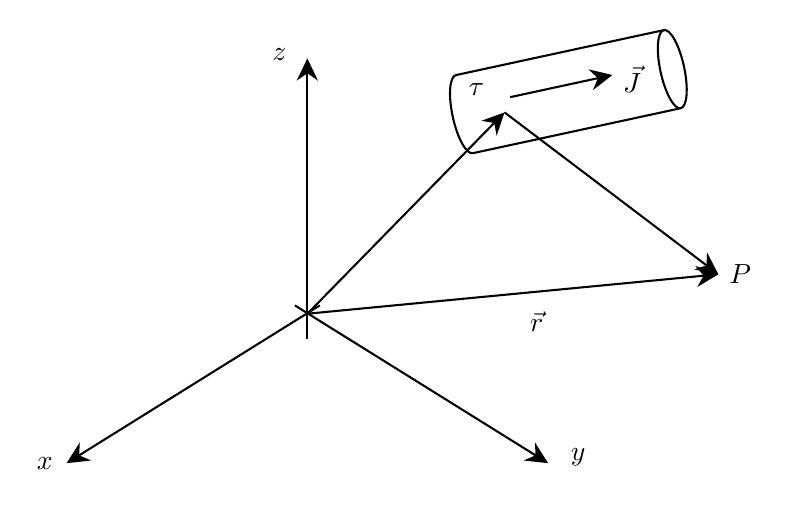
\begin{tikzpicture}[x=0.75pt,y=0.75pt,yscale=-1,xscale=1]
	%uncomment if require: \path (0,300); %set diagram left start at 0, and has height of 300

	%Straight Lines [id:da14089481344117294] 
	\draw    (208.49,184) -- (208.49,52) ;
	\draw [shift={(208.49,49)}, rotate = 450] [fill={rgb, 255:red, 0; green, 0; blue, 0 }  ][line width=0.08]  [draw opacity=0] (10.72,-5.15) -- (0,0) -- (10.72,5.15) -- (7.12,0) -- cycle    ;
	%Straight Lines [id:da04861389550601669] 
	\draw    (202.49,168) -- (321.95,242.41) ;
	\draw [shift={(324.5,244)}, rotate = 211.92000000000002] [fill={rgb, 255:red, 0; green, 0; blue, 0 }  ][line width=0.08]  [draw opacity=0] (10.72,-5.15) -- (0,0) -- (10.72,5.15) -- (7.12,0) -- cycle    ;
	%Straight Lines [id:da28624936293878034] 
	\draw    (214.5,168) -- (95.03,242.41) ;
	\draw [shift={(92.49,244)}, rotate = 328.08000000000004] [fill={rgb, 255:red, 0; green, 0; blue, 0 }  ][line width=0.08]  [draw opacity=0] (10.72,-5.15) -- (0,0) -- (10.72,5.15) -- (7.12,0) -- cycle    ;
	%Straight Lines [id:da8527048498119507] 
	\draw    (208.5,172) -- (403.51,153.29) ;
	\draw [shift={(406.5,153)}, rotate = 534.52] [fill={rgb, 255:red, 0; green, 0; blue, 0 }  ][line width=0.08]  [draw opacity=0] (10.72,-5.15) -- (0,0) -- (10.72,5.15) -- (7.12,0) -- cycle    ;
	%Shape: Can [id:dp4456189893883906] 
	\draw   (388.39,72.98) -- (288.26,94.65) .. controls (285.14,95.32) and (280.79,87.45) .. (278.54,77.06) .. controls (276.29,66.66) and (277,57.69) .. (280.11,57.02) -- (380.24,35.35) .. controls (383.36,34.68) and (387.71,42.55) .. (389.96,52.94) .. controls (392.21,63.34) and (391.5,72.31) .. (388.39,72.98) .. controls (385.27,73.66) and (380.92,65.78) .. (378.67,55.39) .. controls (376.42,45) and (377.13,36.03) .. (380.24,35.35) ;
	%Straight Lines [id:da936996720892316] 
	\draw    (208.5,172) -- (301.4,77.14) ;
	\draw [shift={(303.5,75)}, rotate = 494.4] [fill={rgb, 255:red, 0; green, 0; blue, 0 }  ][line width=0.08]  [draw opacity=0] (10.72,-5.15) -- (0,0) -- (10.72,5.15) -- (7.12,0) -- cycle    ;
	%Straight Lines [id:da6084536348070848] 
	\draw    (303.5,75) -- (404.11,151.19) ;
	\draw [shift={(406.5,153)}, rotate = 217.14] [fill={rgb, 255:red, 0; green, 0; blue, 0 }  ][line width=0.08]  [draw opacity=0] (10.72,-5.15) -- (0,0) -- (10.72,5.15) -- (7.12,0) -- cycle    ;
	%Straight Lines [id:da08362950852228868] 
	\draw    (306.26,67.65) -- (352.53,57.63) ;
	\draw [shift={(355.46,57)}, rotate = 527.79] [fill={rgb, 255:red, 0; green, 0; blue, 0 }  ][line width=0.08]  [draw opacity=0] (10.72,-5.15) -- (0,0) -- (10.72,5.15) -- (7.12,0) -- cycle    ;

	% Text Node
	\draw (319,176) node    {$\vec{r}$};
	% Text Node
	\draw (417,153) node    {$P$};
	% Text Node
	\draw (365,59) node    {$\vec{J}$};
	% Text Node
	\draw (290,64) node    {$\tau $};
	% Text Node
	\draw (82,244) node    {$x$};
	% Text Node
	\draw (339,241) node    {$y$};
	% Text Node
	\draw (195,47) node    {$z$};

	\end{tikzpicture}
\end{figure}
\FloatBarrier

Abbiamo visto che il potenziale vettore $\vec{A}$ è pari a:

\[
	\nabla^2 \vec{A} = -\mu_0 \vec{J}  \implies  \vec{A} (P) = \int_{\tau}\frac{\mu_0 \vec{J} (\vec{r'} )}{4\pi |\vec{r} -\vec{r'} |}d\tau
\]

Possiamo sfruttare questo risultato nel caso di un materiale magnetizzato. Per calcolare il campo magnetico prodotto da questo materiale, possiamo partire dalle correnti di magnetizzazione.

\begin{gather*}
	\vec{J}_m=\vec{M} \times \vec{n} =\text{rot}\vec{M} \\
	\vec{A} (P) = \int_{\tau}\frac{\mu_0 \vec{J}_m  (\vec{r'} )}{4\pi |\vec{r} -\vec{r'} |}d\tau + \int_{\Sigma}\frac{\mu_0 \vec{j}_{sm}  (\vec{r'} )}{4\pi |\vec{r} -\vec{r'} |}dS \qquad \vec{B} =\text{rot}\vec{A}
\end{gather*}

\section{Vettore campo magnetico H, legge di Ampere per H}

Le equazioni generali della magnetostatica nel vuoto devono essere in parte modificate quando sono presenti mezzi magnetizzati. Resta invariata la proprietà di $\vec{B}$ di essere solenoidale mentre cambiano le equazioni in cui compiono le sorgenti, a seguito dell'introduzione delle correnti amperiane. Supponiamo di voler studiare un problema di magnetostatica di carattere generale in cui vi sia un circuito percorso da corrente immerso in un materiale magnetizzato. Vogliamo calcolare il campo induzione magnetica $\vec{B}$ generato da questa configurazione. Consideriamo una linea chiusa concatenata con il filo percorso da corrente. In questa situazione la corrente i non è l'unica concatenata con $\gamma$. Se in prossimità della linea $\gamma$ infatti c'è un atomo, avremo non solo la corrente i ma anche quella microscopica dovuta all'elettrone orbitante. Avremo:

\[
	\oint_{\gamma} \vec{B} \cdot d\vec{l} = \mu_0 I^{\text{conc. a}\gamma}  = \mu_0 (I_{\text{conduzione}}^{\gamma} + I_{\text{magnetizzazione}}^{\gamma}    )
\]

Il campo magnetico generatore dalla corrente di conduzione magnetizza il materiale portando a un cambiamento della sorgente di magnetizzazione, che a sua volta diventa poi sorgente di campo magnetico e a sua volta influenza la magnetizzazione del materiale. Per risolvere il problema ci ricordiamo che:

\begin{gather*}
	\vec{J}_m=\text{rot}\vec{M} \\
	\text{rot}\vec{B} = \mu_0 \vec{J}_{\text{tot}} = \mu_0 (\vec{J} +\vec{J}_m ) = \mu_0 \vec{J} + \mu_0 \,\text{rot}\vec{M}
\end{gather*}

Allora

\begin{align*}
	\text{rot}\frac{\vec{B}}{\mu_0}-\text{rot}\vec{M} &= \vec{J} \\
	\text{rot} \underbrace{\left( \frac{\vec{B}}{\mu_0}-\vec{M} \right)}_{\vec{H}}   &= \vec{J} \implies  \text{rot}\vec{H} = \vec{J}
\end{align*}

Il rotore dipende solo dalle correnti di conduzione che a questo punto sono note. Definiamo questa nuova quantità $\vec{H}$ campo magnetico.

\[
	\boxed{\vec{H} = \frac{\vec{B}}{\mu_0} - \vec{M}} \qquad [H]=[M] \quad \left( \frac{A}{m} \right)
\]

Per il teorema di Stokes a questo punto possiamo passare ad una legge di Ampere per il campo $\vec{H}$. Se consideriamo una linea chiusa $\gamma$ e applichiamo il teorema di Stokes alla superficie $\Sigma$ su cui $\gamma$ si poggia, dimostriamo che la circuitazione lungo $\gamma$ di $\vec{H}$ è uguale alla corrente di circuitazione

\[
	\text{rot}\vec{H} =\vec{J} \implies \oint_{\gamma} \vec{H} \cdot d\vec{l} = I_{\text{conduzione}}
\]

Formalmente la dipendenza dalle correnti amperiane è sparita. In realtà il problema è solo spostato: il loro contributo, nascosto con la riformulazione delle equazioni generali, ricompare nel legame fra $\vec{B}$ ed $ \vec{H}  $. C'è dunque bisogno dell'equazione di stato del mezzo magnetizzato, cioè della relazione specifica fra $\vec{B}$ ed $ \vec{M}  $ o $\vec{B}$ ed $ \vec{H}  $. Nei materiali dia e paramagentici, si verifica che il legame fra il campo $ \vec{H}  $ e la magnetizzazione del materiale è

\[
	\boxed{\vec{M} =\chi_m\vec{H} =(\mu_r -1)\vec{H}}
\]

Possiamo sfruttare questa relazione per determinare il legame fra $\vec{B}$ e $ \vec{H}  $.

\[
	\vec{H} =\frac{\vec{B}}{\mu_0}-\vec{M} \implies \vec{B} =\mu_0 (\vec{H} +\vec{M} )=\mu_0 (\vec{H} + \underbrace{(\mu_r -1)\vec{H}}_{\vec{M}}  ) = \mu_0 (\vec{H} +\mu_r \vec{H} -\vec{H})
\]

\[
	\boxed{\vec{B} =\mu_0 \mu_r \vec{H}}
\]

Nel vuoto, $ \mu_r =1 $.

Avevamo introdotto il solenoide e calcolato il campo di induzione magnetica. Possiamo a questo punto calcolare il campo magnetico come

\[
	\vec{B}_0 = \mu_0 \,n\,I\,\vec{u}_z \qquad \vec{H} =n\,I\,\vec{u}_z
\]

Se riempio il solenoide di materiale dia e paramagnetico $\vec{H}$ non cambia perché dipende solo dalle correnti di conduzione, sul solenoide

\begin{figure}[htpb]
	\centering

	\tikzset{every picture/.style={line width=0.75pt}} %set default line width to 0.75pt        

	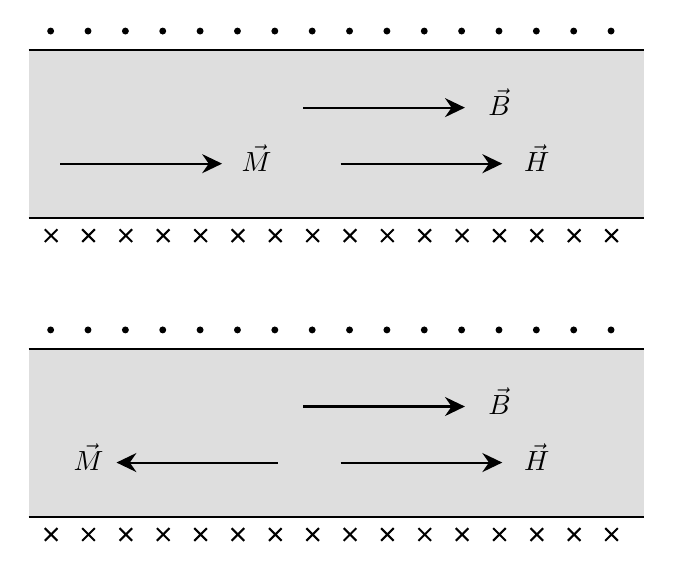
\begin{tikzpicture}[x=0.75pt,y=0.75pt,yscale=-0.9,xscale=0.9]
	%uncomment if require: \path (0,431); %set diagram left start at 0, and has height of 431

	%Shape: Rectangle [id:dp6427071080625504] 
	\draw  [draw opacity=0][fill={rgb, 255:red, 222; green, 222; blue, 222 }  ,fill opacity=1 ] (96,68.75) -- (425.5,68.75) -- (425.5,158.75) -- (96,158.75) -- cycle ;
	%Straight Lines [id:da02536138059326687] 
	\draw    (96,68.75) -- (425.5,68.75) ;
	%Shape: Circle [id:dp1826177540774201] 
	\draw  [fill={rgb, 255:red, 0; green, 0; blue, 0 }  ,fill opacity=1 ] (106.5,58.75) .. controls (106.5,58.06) and (107.06,57.5) .. (107.75,57.5) .. controls (108.44,57.5) and (109,58.06) .. (109,58.75) .. controls (109,59.44) and (108.44,60) .. (107.75,60) .. controls (107.06,60) and (106.5,59.44) .. (106.5,58.75) -- cycle ;
	%Straight Lines [id:da7226876699060629] 
	\draw    (243,99.75) -- (326.5,99.75) ;
	\draw [shift={(329.5,99.75)}, rotate = 180] [fill={rgb, 255:red, 0; green, 0; blue, 0 }  ][line width=0.08]  [draw opacity=0] (10.72,-5.15) -- (0,0) -- (10.72,5.15) -- (7.12,0) -- cycle    ;
	%Shape: Circle [id:dp135714257827928] 
	\draw  [fill={rgb, 255:red, 0; green, 0; blue, 0 }  ,fill opacity=1 ] (126.5,58.75) .. controls (126.5,58.06) and (127.06,57.5) .. (127.75,57.5) .. controls (128.44,57.5) and (129,58.06) .. (129,58.75) .. controls (129,59.44) and (128.44,60) .. (127.75,60) .. controls (127.06,60) and (126.5,59.44) .. (126.5,58.75) -- cycle ;
	%Shape: Circle [id:dp8414141297589808] 
	\draw  [fill={rgb, 255:red, 0; green, 0; blue, 0 }  ,fill opacity=1 ] (146.5,58.75) .. controls (146.5,58.06) and (147.06,57.5) .. (147.75,57.5) .. controls (148.44,57.5) and (149,58.06) .. (149,58.75) .. controls (149,59.44) and (148.44,60) .. (147.75,60) .. controls (147.06,60) and (146.5,59.44) .. (146.5,58.75) -- cycle ;
	%Shape: Circle [id:dp06458340832650489] 
	\draw  [fill={rgb, 255:red, 0; green, 0; blue, 0 }  ,fill opacity=1 ] (166.5,58.75) .. controls (166.5,58.06) and (167.06,57.5) .. (167.75,57.5) .. controls (168.44,57.5) and (169,58.06) .. (169,58.75) .. controls (169,59.44) and (168.44,60) .. (167.75,60) .. controls (167.06,60) and (166.5,59.44) .. (166.5,58.75) -- cycle ;
	%Shape: Circle [id:dp9955754546391007] 
	\draw  [fill={rgb, 255:red, 0; green, 0; blue, 0 }  ,fill opacity=1 ] (186.5,58.75) .. controls (186.5,58.06) and (187.06,57.5) .. (187.75,57.5) .. controls (188.44,57.5) and (189,58.06) .. (189,58.75) .. controls (189,59.44) and (188.44,60) .. (187.75,60) .. controls (187.06,60) and (186.5,59.44) .. (186.5,58.75) -- cycle ;
	%Shape: Circle [id:dp6562179670055472] 
	\draw  [fill={rgb, 255:red, 0; green, 0; blue, 0 }  ,fill opacity=1 ] (206.5,58.75) .. controls (206.5,58.06) and (207.06,57.5) .. (207.75,57.5) .. controls (208.44,57.5) and (209,58.06) .. (209,58.75) .. controls (209,59.44) and (208.44,60) .. (207.75,60) .. controls (207.06,60) and (206.5,59.44) .. (206.5,58.75) -- cycle ;
	%Shape: Circle [id:dp30873013575036934] 
	\draw  [fill={rgb, 255:red, 0; green, 0; blue, 0 }  ,fill opacity=1 ] (226.5,58.75) .. controls (226.5,58.06) and (227.06,57.5) .. (227.75,57.5) .. controls (228.44,57.5) and (229,58.06) .. (229,58.75) .. controls (229,59.44) and (228.44,60) .. (227.75,60) .. controls (227.06,60) and (226.5,59.44) .. (226.5,58.75) -- cycle ;
	%Shape: Circle [id:dp41591900705823415] 
	\draw  [fill={rgb, 255:red, 0; green, 0; blue, 0 }  ,fill opacity=1 ] (246.5,58.75) .. controls (246.5,58.06) and (247.06,57.5) .. (247.75,57.5) .. controls (248.44,57.5) and (249,58.06) .. (249,58.75) .. controls (249,59.44) and (248.44,60) .. (247.75,60) .. controls (247.06,60) and (246.5,59.44) .. (246.5,58.75) -- cycle ;
	%Shape: Circle [id:dp9266837575895301] 
	\draw  [fill={rgb, 255:red, 0; green, 0; blue, 0 }  ,fill opacity=1 ] (266.5,58.75) .. controls (266.5,58.06) and (267.06,57.5) .. (267.75,57.5) .. controls (268.44,57.5) and (269,58.06) .. (269,58.75) .. controls (269,59.44) and (268.44,60) .. (267.75,60) .. controls (267.06,60) and (266.5,59.44) .. (266.5,58.75) -- cycle ;
	%Shape: Circle [id:dp28704927034916183] 
	\draw  [fill={rgb, 255:red, 0; green, 0; blue, 0 }  ,fill opacity=1 ] (286.5,58.75) .. controls (286.5,58.06) and (287.06,57.5) .. (287.75,57.5) .. controls (288.44,57.5) and (289,58.06) .. (289,58.75) .. controls (289,59.44) and (288.44,60) .. (287.75,60) .. controls (287.06,60) and (286.5,59.44) .. (286.5,58.75) -- cycle ;
	%Shape: Circle [id:dp6496748933975611] 
	\draw  [fill={rgb, 255:red, 0; green, 0; blue, 0 }  ,fill opacity=1 ] (306.5,58.75) .. controls (306.5,58.06) and (307.06,57.5) .. (307.75,57.5) .. controls (308.44,57.5) and (309,58.06) .. (309,58.75) .. controls (309,59.44) and (308.44,60) .. (307.75,60) .. controls (307.06,60) and (306.5,59.44) .. (306.5,58.75) -- cycle ;
	%Shape: Circle [id:dp7774682231925598] 
	\draw  [fill={rgb, 255:red, 0; green, 0; blue, 0 }  ,fill opacity=1 ] (326.5,58.75) .. controls (326.5,58.06) and (327.06,57.5) .. (327.75,57.5) .. controls (328.44,57.5) and (329,58.06) .. (329,58.75) .. controls (329,59.44) and (328.44,60) .. (327.75,60) .. controls (327.06,60) and (326.5,59.44) .. (326.5,58.75) -- cycle ;
	%Shape: Circle [id:dp5127696851811765] 
	\draw  [fill={rgb, 255:red, 0; green, 0; blue, 0 }  ,fill opacity=1 ] (346.5,58.75) .. controls (346.5,58.06) and (347.06,57.5) .. (347.75,57.5) .. controls (348.44,57.5) and (349,58.06) .. (349,58.75) .. controls (349,59.44) and (348.44,60) .. (347.75,60) .. controls (347.06,60) and (346.5,59.44) .. (346.5,58.75) -- cycle ;
	%Shape: Circle [id:dp5825232050499962] 
	\draw  [fill={rgb, 255:red, 0; green, 0; blue, 0 }  ,fill opacity=1 ] (366.5,58.75) .. controls (366.5,58.06) and (367.06,57.5) .. (367.75,57.5) .. controls (368.44,57.5) and (369,58.06) .. (369,58.75) .. controls (369,59.44) and (368.44,60) .. (367.75,60) .. controls (367.06,60) and (366.5,59.44) .. (366.5,58.75) -- cycle ;
	%Shape: Circle [id:dp8202403521275767] 
	\draw  [fill={rgb, 255:red, 0; green, 0; blue, 0 }  ,fill opacity=1 ] (386.5,58.75) .. controls (386.5,58.06) and (387.06,57.5) .. (387.75,57.5) .. controls (388.44,57.5) and (389,58.06) .. (389,58.75) .. controls (389,59.44) and (388.44,60) .. (387.75,60) .. controls (387.06,60) and (386.5,59.44) .. (386.5,58.75) -- cycle ;
	%Shape: Circle [id:dp7808710947800921] 
	\draw  [fill={rgb, 255:red, 0; green, 0; blue, 0 }  ,fill opacity=1 ] (406.5,58.75) .. controls (406.5,58.06) and (407.06,57.5) .. (407.75,57.5) .. controls (408.44,57.5) and (409,58.06) .. (409,58.75) .. controls (409,59.44) and (408.44,60) .. (407.75,60) .. controls (407.06,60) and (406.5,59.44) .. (406.5,58.75) -- cycle ;
	\draw   (104.62,164.88) -- (111.38,171.63)(111.38,164.88) -- (104.63,171.63) ;
	\draw   (124.62,164.88) -- (131.38,171.63)(131.38,164.88) -- (124.63,171.63) ;
	\draw   (144.63,164.88) -- (151.38,171.63)(151.38,164.88) -- (144.63,171.63) ;
	\draw   (164.63,164.88) -- (171.38,171.63)(171.38,164.88) -- (164.63,171.63) ;
	\draw   (184.63,164.88) -- (191.38,171.63)(191.38,164.88) -- (184.63,171.63) ;
	\draw   (204.63,164.88) -- (211.38,171.63)(211.38,164.88) -- (204.63,171.63) ;
	\draw   (224.63,164.88) -- (231.38,171.63)(231.38,164.88) -- (224.63,171.63) ;
	\draw   (244.63,164.88) -- (251.38,171.63)(251.38,164.88) -- (244.63,171.63) ;
	\draw   (264.63,164.88) -- (271.38,171.63)(271.38,164.88) -- (264.63,171.63) ;
	\draw   (284.63,164.88) -- (291.38,171.63)(291.38,164.88) -- (284.63,171.63) ;
	\draw   (304.63,164.88) -- (311.38,171.63)(311.38,164.88) -- (304.63,171.63) ;
	\draw   (324.63,164.88) -- (331.38,171.63)(331.38,164.88) -- (324.63,171.63) ;
	\draw   (344.63,164.88) -- (351.38,171.63)(351.38,164.88) -- (344.63,171.63) ;
	\draw   (364.63,164.88) -- (371.38,171.63)(371.38,164.88) -- (364.63,171.63) ;
	\draw   (384.63,164.88) -- (391.38,171.63)(391.38,164.88) -- (384.63,171.63) ;
	\draw   (404.63,164.88) -- (411.38,171.63)(411.38,164.88) -- (404.63,171.63) ;
	%Straight Lines [id:da5515374168158742] 
	\draw    (96,158.75) -- (425.5,158.75) ;
	%Straight Lines [id:da6001340342286905] 
	\draw    (263,129.75) -- (346.5,129.75) ;
	\draw [shift={(349.5,129.75)}, rotate = 180] [fill={rgb, 255:red, 0; green, 0; blue, 0 }  ][line width=0.08]  [draw opacity=0] (10.72,-5.15) -- (0,0) -- (10.72,5.15) -- (7.12,0) -- cycle    ;
	%Straight Lines [id:da688135203676403] 
	\draw    (113,129.75) -- (196.5,129.75) ;
	\draw [shift={(199.5,129.75)}, rotate = 180] [fill={rgb, 255:red, 0; green, 0; blue, 0 }  ][line width=0.08]  [draw opacity=0] (10.72,-5.15) -- (0,0) -- (10.72,5.15) -- (7.12,0) -- cycle    ;
	%Shape: Rectangle [id:dp4520732820043767] 
	\draw  [draw opacity=0][fill={rgb, 255:red, 222; green, 222; blue, 222 }  ,fill opacity=1 ] (96,228.75) -- (425.5,228.75) -- (425.5,318.75) -- (96,318.75) -- cycle ;
	%Straight Lines [id:da31695156333379804] 
	\draw    (96,228.75) -- (425.5,228.75) ;
	%Shape: Circle [id:dp058683178208204234] 
	\draw  [fill={rgb, 255:red, 0; green, 0; blue, 0 }  ,fill opacity=1 ] (106.5,218.75) .. controls (106.5,218.06) and (107.06,217.5) .. (107.75,217.5) .. controls (108.44,217.5) and (109,218.06) .. (109,218.75) .. controls (109,219.44) and (108.44,220) .. (107.75,220) .. controls (107.06,220) and (106.5,219.44) .. (106.5,218.75) -- cycle ;
	%Straight Lines [id:da13910800112872845] 
	\draw    (243,259.75) -- (326.5,259.75) ;
	\draw [shift={(329.5,259.75)}, rotate = 180] [fill={rgb, 255:red, 0; green, 0; blue, 0 }  ][line width=0.08]  [draw opacity=0] (10.72,-5.15) -- (0,0) -- (10.72,5.15) -- (7.12,0) -- cycle    ;
	%Shape: Circle [id:dp26864700409227416] 
	\draw  [fill={rgb, 255:red, 0; green, 0; blue, 0 }  ,fill opacity=1 ] (126.5,218.75) .. controls (126.5,218.06) and (127.06,217.5) .. (127.75,217.5) .. controls (128.44,217.5) and (129,218.06) .. (129,218.75) .. controls (129,219.44) and (128.44,220) .. (127.75,220) .. controls (127.06,220) and (126.5,219.44) .. (126.5,218.75) -- cycle ;
	%Shape: Circle [id:dp23855630787270687] 
	\draw  [fill={rgb, 255:red, 0; green, 0; blue, 0 }  ,fill opacity=1 ] (146.5,218.75) .. controls (146.5,218.06) and (147.06,217.5) .. (147.75,217.5) .. controls (148.44,217.5) and (149,218.06) .. (149,218.75) .. controls (149,219.44) and (148.44,220) .. (147.75,220) .. controls (147.06,220) and (146.5,219.44) .. (146.5,218.75) -- cycle ;
	%Shape: Circle [id:dp9682794279453872] 
	\draw  [fill={rgb, 255:red, 0; green, 0; blue, 0 }  ,fill opacity=1 ] (166.5,218.75) .. controls (166.5,218.06) and (167.06,217.5) .. (167.75,217.5) .. controls (168.44,217.5) and (169,218.06) .. (169,218.75) .. controls (169,219.44) and (168.44,220) .. (167.75,220) .. controls (167.06,220) and (166.5,219.44) .. (166.5,218.75) -- cycle ;
	%Shape: Circle [id:dp9013656584078027] 
	\draw  [fill={rgb, 255:red, 0; green, 0; blue, 0 }  ,fill opacity=1 ] (186.5,218.75) .. controls (186.5,218.06) and (187.06,217.5) .. (187.75,217.5) .. controls (188.44,217.5) and (189,218.06) .. (189,218.75) .. controls (189,219.44) and (188.44,220) .. (187.75,220) .. controls (187.06,220) and (186.5,219.44) .. (186.5,218.75) -- cycle ;
	%Shape: Circle [id:dp30744533236881044] 
	\draw  [fill={rgb, 255:red, 0; green, 0; blue, 0 }  ,fill opacity=1 ] (206.5,218.75) .. controls (206.5,218.06) and (207.06,217.5) .. (207.75,217.5) .. controls (208.44,217.5) and (209,218.06) .. (209,218.75) .. controls (209,219.44) and (208.44,220) .. (207.75,220) .. controls (207.06,220) and (206.5,219.44) .. (206.5,218.75) -- cycle ;
	%Shape: Circle [id:dp8567039311674027] 
	\draw  [fill={rgb, 255:red, 0; green, 0; blue, 0 }  ,fill opacity=1 ] (226.5,218.75) .. controls (226.5,218.06) and (227.06,217.5) .. (227.75,217.5) .. controls (228.44,217.5) and (229,218.06) .. (229,218.75) .. controls (229,219.44) and (228.44,220) .. (227.75,220) .. controls (227.06,220) and (226.5,219.44) .. (226.5,218.75) -- cycle ;
	%Shape: Circle [id:dp9957234165699325] 
	\draw  [fill={rgb, 255:red, 0; green, 0; blue, 0 }  ,fill opacity=1 ] (246.5,218.75) .. controls (246.5,218.06) and (247.06,217.5) .. (247.75,217.5) .. controls (248.44,217.5) and (249,218.06) .. (249,218.75) .. controls (249,219.44) and (248.44,220) .. (247.75,220) .. controls (247.06,220) and (246.5,219.44) .. (246.5,218.75) -- cycle ;
	%Shape: Circle [id:dp34454506519841854] 
	\draw  [fill={rgb, 255:red, 0; green, 0; blue, 0 }  ,fill opacity=1 ] (266.5,218.75) .. controls (266.5,218.06) and (267.06,217.5) .. (267.75,217.5) .. controls (268.44,217.5) and (269,218.06) .. (269,218.75) .. controls (269,219.44) and (268.44,220) .. (267.75,220) .. controls (267.06,220) and (266.5,219.44) .. (266.5,218.75) -- cycle ;
	%Shape: Circle [id:dp7997299928263821] 
	\draw  [fill={rgb, 255:red, 0; green, 0; blue, 0 }  ,fill opacity=1 ] (286.5,218.75) .. controls (286.5,218.06) and (287.06,217.5) .. (287.75,217.5) .. controls (288.44,217.5) and (289,218.06) .. (289,218.75) .. controls (289,219.44) and (288.44,220) .. (287.75,220) .. controls (287.06,220) and (286.5,219.44) .. (286.5,218.75) -- cycle ;
	%Shape: Circle [id:dp6688245831598758] 
	\draw  [fill={rgb, 255:red, 0; green, 0; blue, 0 }  ,fill opacity=1 ] (306.5,218.75) .. controls (306.5,218.06) and (307.06,217.5) .. (307.75,217.5) .. controls (308.44,217.5) and (309,218.06) .. (309,218.75) .. controls (309,219.44) and (308.44,220) .. (307.75,220) .. controls (307.06,220) and (306.5,219.44) .. (306.5,218.75) -- cycle ;
	%Shape: Circle [id:dp4250502639100042] 
	\draw  [fill={rgb, 255:red, 0; green, 0; blue, 0 }  ,fill opacity=1 ] (326.5,218.75) .. controls (326.5,218.06) and (327.06,217.5) .. (327.75,217.5) .. controls (328.44,217.5) and (329,218.06) .. (329,218.75) .. controls (329,219.44) and (328.44,220) .. (327.75,220) .. controls (327.06,220) and (326.5,219.44) .. (326.5,218.75) -- cycle ;
	%Shape: Circle [id:dp8969147365794026] 
	\draw  [fill={rgb, 255:red, 0; green, 0; blue, 0 }  ,fill opacity=1 ] (346.5,218.75) .. controls (346.5,218.06) and (347.06,217.5) .. (347.75,217.5) .. controls (348.44,217.5) and (349,218.06) .. (349,218.75) .. controls (349,219.44) and (348.44,220) .. (347.75,220) .. controls (347.06,220) and (346.5,219.44) .. (346.5,218.75) -- cycle ;
	%Shape: Circle [id:dp2579939119887864] 
	\draw  [fill={rgb, 255:red, 0; green, 0; blue, 0 }  ,fill opacity=1 ] (366.5,218.75) .. controls (366.5,218.06) and (367.06,217.5) .. (367.75,217.5) .. controls (368.44,217.5) and (369,218.06) .. (369,218.75) .. controls (369,219.44) and (368.44,220) .. (367.75,220) .. controls (367.06,220) and (366.5,219.44) .. (366.5,218.75) -- cycle ;
	%Shape: Circle [id:dp9467759531843045] 
	\draw  [fill={rgb, 255:red, 0; green, 0; blue, 0 }  ,fill opacity=1 ] (386.5,218.75) .. controls (386.5,218.06) and (387.06,217.5) .. (387.75,217.5) .. controls (388.44,217.5) and (389,218.06) .. (389,218.75) .. controls (389,219.44) and (388.44,220) .. (387.75,220) .. controls (387.06,220) and (386.5,219.44) .. (386.5,218.75) -- cycle ;
	%Shape: Circle [id:dp15470905220593067] 
	\draw  [fill={rgb, 255:red, 0; green, 0; blue, 0 }  ,fill opacity=1 ] (406.5,218.75) .. controls (406.5,218.06) and (407.06,217.5) .. (407.75,217.5) .. controls (408.44,217.5) and (409,218.06) .. (409,218.75) .. controls (409,219.44) and (408.44,220) .. (407.75,220) .. controls (407.06,220) and (406.5,219.44) .. (406.5,218.75) -- cycle ;
	\draw   (104.62,324.88) -- (111.38,331.63)(111.38,324.88) -- (104.63,331.63) ;
	\draw   (124.62,324.88) -- (131.38,331.63)(131.38,324.88) -- (124.63,331.63) ;
	\draw   (144.63,324.88) -- (151.38,331.63)(151.38,324.88) -- (144.63,331.63) ;
	\draw   (164.63,324.88) -- (171.38,331.63)(171.38,324.88) -- (164.63,331.63) ;
	\draw   (184.63,324.88) -- (191.38,331.63)(191.38,324.88) -- (184.63,331.63) ;
	\draw   (204.63,324.88) -- (211.38,331.63)(211.38,324.88) -- (204.63,331.63) ;
	\draw   (224.63,324.88) -- (231.38,331.63)(231.38,324.88) -- (224.63,331.63) ;
	\draw   (244.63,324.88) -- (251.38,331.63)(251.38,324.88) -- (244.63,331.63) ;
	\draw   (264.63,324.88) -- (271.38,331.63)(271.38,324.88) -- (264.63,331.63) ;
	\draw   (284.63,324.88) -- (291.38,331.63)(291.38,324.88) -- (284.63,331.63) ;
	\draw   (304.63,324.88) -- (311.38,331.63)(311.38,324.88) -- (304.63,331.63) ;
	\draw   (324.63,324.88) -- (331.38,331.63)(331.38,324.88) -- (324.63,331.63) ;
	\draw   (344.63,324.88) -- (351.38,331.63)(351.38,324.88) -- (344.63,331.63) ;
	\draw   (364.63,324.88) -- (371.38,331.63)(371.38,324.88) -- (364.63,331.63) ;
	\draw   (384.63,324.88) -- (391.38,331.63)(391.38,324.88) -- (384.63,331.63) ;
	\draw   (404.63,324.88) -- (411.38,331.63)(411.38,324.88) -- (404.63,331.63) ;
	%Straight Lines [id:da8339849913610828] 
	\draw    (96,318.75) -- (425.5,318.75) ;
	%Straight Lines [id:da14389562494957642] 
	\draw    (263,289.75) -- (346.5,289.75) ;
	\draw [shift={(349.5,289.75)}, rotate = 180] [fill={rgb, 255:red, 0; green, 0; blue, 0 }  ][line width=0.08]  [draw opacity=0] (10.72,-5.15) -- (0,0) -- (10.72,5.15) -- (7.12,0) -- cycle    ;
	%Straight Lines [id:da29226931720777194] 
	\draw    (146,289.75) -- (229.5,289.75) ;
	\draw [shift={(143,289.75)}, rotate = 0] [fill={rgb, 255:red, 0; green, 0; blue, 0 }  ][line width=0.08]  [draw opacity=0] (10.72,-5.15) -- (0,0) -- (10.72,5.15) -- (7.12,0) -- cycle    ;

	% Text Node
	\draw (348,96.75) node    {$\vec{B}$};
	% Text Node
	\draw (368,126.75) node    {$\vec{H}$};
	% Text Node
	\draw (218,126.75) node    {$\vec{M}$};
	% Text Node
	\draw (348,256.75) node    {$\vec{B}$};
	% Text Node
	\draw (368,286.75) node    {$\vec{H}$};
	% Text Node
	\draw (128,286.75) node    {$\vec{M}$};

	\end{tikzpicture}
\end{figure}
\FloatBarrier

In particolare, se il materiale è diamagnetico $\xi_m $è negativo e quindi $\vec{H}$ sarà diretto in verso opposto a $\vec{M}$.
Nei materiali diamagnetici l'unico effetto di magnetizzazione dominante è quello del processo di Larmor. Il momento magnetico di Larmor è diretto in verso opposto rispetto a $\vec{M}$. Ecco perché in questi materiali $\vec{H}$ è diretto in verso opposto.
Nei materiali paramagnetici il processo dominante è quello di magnetizzazione per orientamento. I dipoli si orientano nel verso del campo $\vec{B}$ e quindi anche $\vec{H}$ sarà diretto come $\vec{B}$.

\section{Ciclo di isteresi}

Nei materiali ferromagnetici la situazione è molto più complessa. D'altra parte è nelle sostanze ferromagnetiche che gli effetti sono notevoli e rivestono importantissimi aspetti tecnologici, per cui il loro studio è molto utile. In essi $\xi_m$ è una funzione non univoca di $\vec{H}$ e non si può parlare di equazione di stato in termini semplici. La relazione tra $\vec{M}$ ed $\vec{H}$ o $\vec{B}$ ed $\vec{H}$ è espressa tramite il \textbf{ciclo di isteresi}. Le proprietà magnetiche delle leghe variano notevolmente con la composizione chimica e dipendono anche dai trattamenti termici subiti. Infine per alcune leghe speciali le proprietà magnetiche possono cambiare radicalmente sotto sollecitazioni meccaniche esterne. Tutti questi fatti inducono a ritenere che i fenomeni atomici che stanno alla base del ferromagnetismo dipendano fortemente dalla struttura cristallina e dalle sue modificazioni causate da agenti termici o meccanici. Supponiamo che inizialmente il materiale si trovi nello stato vergine, cioè non sia mai stato sottoposto a magnetizzazione, e che siano nulli tutti i campi (ci troviamo nel punto $0$ del grafico sottostante).
Facendo crescere $\vec{H}$ i valori di $\vec{B}$ e di $\vec{M}$ si dispongono lungo la curva a, detta curva di prima magnetizzazione. Quando $\vec{H}$ supera un certo valore $\vec{H}_m$ la magnetizzazione resta costante al valore $\vec{M}_{\text{sat}}$ e il campo magnetico cresce linearmente con $\vec{H}$, molto più lentamente di prima $(\vec{B} =\mu_0 (\vec{H} +\vec{M}_{\text{sat}}))$. Si dice che per $\vec{H}>\vec{H}_m$ il materiale ha raggiunto la saturazione e il valore $\vec{M}_{\text{sat}}$ si chiama magnetizzazione di saturazione. Non essendo a una retta, i valori $\mu_r$, $\mu_0$ non sono costanti, ma funzioni di $\vec{H}$. Se dopo aver raggiunto il valore $\vec{H}_m$ si fa decrescere $\vec{H}$, i valori di $\vec{B}$ e di $\vec{M}$ si dispongono lungo una nuova curva b che si mantiene al di sopra della curva di prima magnetizzazione e interseca l'asse delle ordinate ($\vec{H}=0$) con il valore $\vec{M}_r$, tale che $B_r=\mu_0 M_r$. Si parla di magnetizzazione residua e di campo magnetico residuo, a significare il fatto fondamentale che il materiale è magnetizzato anche in assenza di corrente; è diventato cioè un magnete permanente. Per annullare la magnetizzazione bisogna invertire il senso della corrente e far diminuire $\vec{H}$ fino ad $\vec{H}_c$, detto campo coercitivo, in corrispondenza del quale $\vec{M}=0$ e $B=\mu_0 H_c$.
Facendo ulteriormente decrescere $\vec{H}$ si osserva che oltre il valore $-\vec{H}_m$ la curva è rettilinea, come lo era oltre $\vec{H}_m$, con stessa pendenza. Il materiale ha raggiunto la magnetizzazione di saturazione, ma con verso opposto.
Infine, se si riporta $\vec{H}$ al valore $\vec{H}_m$ si percorre la curva $c$ fino al ricongiungimento con la curva $a$. La curva completa prende il nome di ciclo di isteresi del materiale.

\begin{figure}[htpb]
	\centering

	\tikzset{every picture/.style={line width=0.75pt}} %set default line width to 0.75pt        

	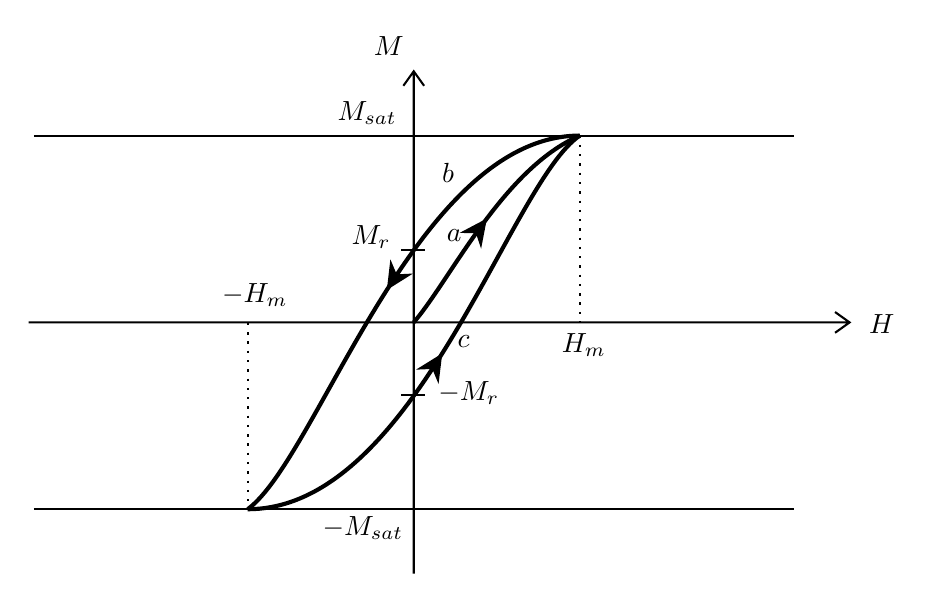
\begin{tikzpicture}[x=0.75pt,y=0.75pt,yscale=-1,xscale=1]
	%uncomment if require: \path (0,300); %set diagram left start at 0, and has height of 300

	%Shape: Axis 2D [id:dp7150192778192135] 
	\draw  (86,158) -- (481.5,158)(271.5,37) -- (271.5,279) (474.5,153) -- (481.5,158) -- (474.5,163) (266.5,44) -- (271.5,37) -- (276.5,44)  ;
	%Straight Lines [id:da1542418627500033] 
	\draw    (88.5,68) -- (454.5,68) ;
	%Straight Lines [id:da4097895049464837] 
	\draw    (88.5,248) -- (454.5,248) ;
	%Curve Lines [id:da521997541674877] 
	\draw [line width=1.5]    (191.5,248) .. controls (272.5,248) and (317.5,91) .. (351.5,68) ;
	\draw [shift={(285.24,172.92)}, rotate = 482.5] [fill={rgb, 255:red, 0; green, 0; blue, 0 }  ][line width=0.08]  [draw opacity=0] (13.4,-6.43) -- (0,0) -- (13.4,6.44) -- (8.9,0) -- cycle    ;
	%Curve Lines [id:da8933862632419602] 
	\draw [line width=1.5]    (191.5,248) .. controls (225.5,223) and (272.5,68) .. (351.5,68) ;
	\draw [shift={(258.55,142.37)}, rotate = 302.19] [fill={rgb, 255:red, 0; green, 0; blue, 0 }  ][line width=0.08]  [draw opacity=0] (13.4,-6.43) -- (0,0) -- (13.4,6.44) -- (8.9,0) -- cycle    ;
	%Curve Lines [id:da9894547116068164] 
	\draw [line width=1.5]    (271.5,158) .. controls (289.5,137) and (314.5,84) .. (351.5,68) ;
	\draw [shift={(306.76,107.92)}, rotate = 486.48] [fill={rgb, 255:red, 0; green, 0; blue, 0 }  ][line width=0.08]  [draw opacity=0] (13.4,-6.43) -- (0,0) -- (13.4,6.44) -- (8.9,0) -- cycle    ;
	%Straight Lines [id:da5888682740936091] 
	\draw    (265.5,123) -- (277,123) ;
	%Straight Lines [id:da5547878679057141] 
	\draw  [dash pattern={on 0.84pt off 2.51pt}]  (351.5,68) -- (351.5,157.75) ;
	%Straight Lines [id:da8719290944587592] 
	\draw  [dash pattern={on 0.84pt off 2.51pt}]  (191.5,158.25) -- (191.5,248) ;
	%Straight Lines [id:da28884191057946706] 
	\draw    (265.5,193) -- (277,193) ;

	% Text Node
	\draw (497,159) node    {$H$};
	% Text Node
	\draw (259.5,25) node    {$M$};
	% Text Node
	\draw (251,117) node    {$M_{r}$};
	% Text Node
	\draw (291,116) node    {$a$};
	% Text Node
	\draw (288,86) node    {$b$};
	% Text Node
	\draw (295.5,167) node    {$c$};
	% Text Node
	\draw (353.5,169) node    {$H_{m}$};
	% Text Node
	\draw (249,57) node    {$M_{sat}$};
	% Text Node
	\draw (247,257) node    {$-M_{sat}$};
	% Text Node
	\draw (195,145) node    {$-H_{m}$};
	% Text Node
	\draw (298,192) node    {$-M_{r}$};

	\end{tikzpicture}
\end{figure}
\FloatBarrier

Finché $\vec{H}$ varia nell'intervallo $-\vec{H}_m$, $\vec{H}_m$ o maggiore si ottiene sempre lo stesso ciclo; se si riduce l'intervallo di variabilità si ottengono cicli più stretti, con i vertici sulla curva di prima magnetizzazione. È questo il metodo che si utilizza in pratica per smagnetizzare un materiale. Uno stato $(H,M)$ può coincidere con un punto del ciclo solo se viene seguita la procedura descritta. Operando in modo opportuno tutti i punti interni al ciclo sono in realtà raggiungibili e il ciclo delimita quindi una regione luogo dei possibili stati del sistema. Ad un dato valore di $\vec{H}$ possono corrispondere infiniti valori di $\vec{B}$ compresi tra le curve $b$ e $c$, situazione che viene riassunta dicendo che la magnetizzazione di una sostanza ferromagnetica dipende dalla storia della sostanza, oltre che dal valore di $\vec{H}$.

La forma del ciclo di isteresi dipende fortemente dalla composizione della sostanza. Vi sono i materiali duri, il cui ciclo è piuttosto largo. Essi sono adatti per la costruzione di magneti permanenti, dato che è difficile smagnetizzarli. Nella situazione opposta vi sono i materiali cosiddetti dolci, che hanno un ciclo di isteresi molto stretto: è facile magnetizzarli e smagnetizzarli.

\section{Linee di flusso per il campo H}

Vediamo cosa possiamo dire circa la divergenza di $\vec{H}$.

\[
	\text{div}\vec{H} =\text{div}\left( \frac{\vec{B}}{\mu_0}-\vec{M}  \right) = \frac{1}{\mu_0} \underbrace{\text{div}\vec{B}}_{=0}-\text{div}\vec{M} \implies \text{div}\vec{H} = - \text{div}\vec{M}
\]

La divergenza di $\vec{H}$ può essere diversa da zero. $\vec{H}$ può avere linee aperte come il campo elettrico. Consideriamo un magnete permanente. Le due facce del magente sono sorgenti delle linee di flusso per $\vec{M}$. Le linee di flusso di $\vec{H}$ si comporteranno come in figura.

\begin{figure}[htpb]
	\centering

	\tikzset{every picture/.style={line width=0.75pt}} %set default line width to 0.75pt        

	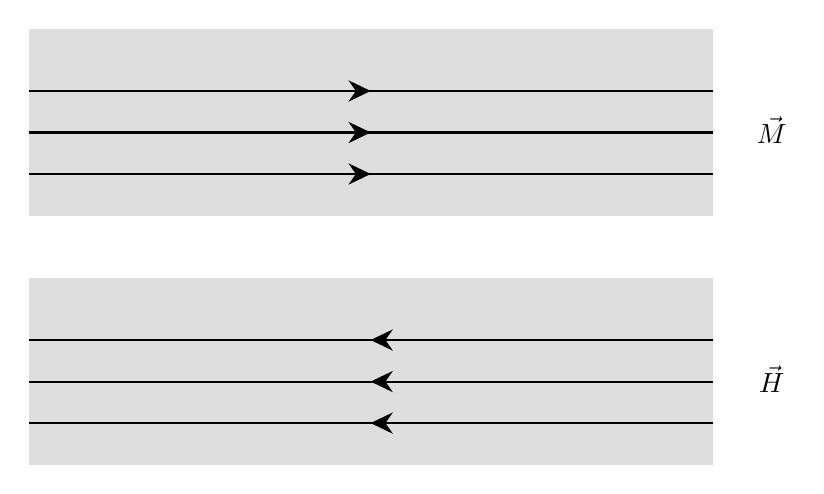
\begin{tikzpicture}[x=0.75pt,y=0.75pt,yscale=-1,xscale=1]
	%uncomment if require: \path (0,300); %set diagram left start at 0, and has height of 300

	%Shape: Rectangle [id:dp8343549760267048] 
	\draw  [draw opacity=0][fill={rgb, 255:red, 222; green, 222; blue, 222 }  ,fill opacity=1 ] (117,59) -- (446.5,59) -- (446.5,149) -- (117,149) -- cycle ;
	%Straight Lines [id:da47270082054582674] 
	\draw    (117,129) -- (446.5,129) ;
	\draw [shift={(281.75,129)}, rotate = 180] [fill={rgb, 255:red, 0; green, 0; blue, 0 }  ][line width=0.08]  [draw opacity=0] (10.72,-5.15) -- (0,0) -- (10.72,5.15) -- (7.12,0) -- cycle    ;
	%Straight Lines [id:da4095153772938622] 
	\draw    (117,109) -- (446.5,109) ;
	\draw [shift={(281.75,109)}, rotate = 180] [fill={rgb, 255:red, 0; green, 0; blue, 0 }  ][line width=0.08]  [draw opacity=0] (10.72,-5.15) -- (0,0) -- (10.72,5.15) -- (7.12,0) -- cycle    ;
	%Straight Lines [id:da7123076971216014] 
	\draw    (117,89) -- (446.5,89) ;
	\draw [shift={(281.75,89)}, rotate = 180] [fill={rgb, 255:red, 0; green, 0; blue, 0 }  ][line width=0.08]  [draw opacity=0] (10.72,-5.15) -- (0,0) -- (10.72,5.15) -- (7.12,0) -- cycle    ;
	%Shape: Rectangle [id:dp8459906698264861] 
	\draw  [draw opacity=0][fill={rgb, 255:red, 222; green, 222; blue, 222 }  ,fill opacity=1 ] (117,179) -- (446.5,179) -- (446.5,269) -- (117,269) -- cycle ;
	%Straight Lines [id:da7887881287067753] 
	\draw    (117,249) -- (446.5,249) ;
	\draw [shift={(281.75,249)}, rotate = 0] [fill={rgb, 255:red, 0; green, 0; blue, 0 }  ][line width=0.08]  [draw opacity=0] (10.72,-5.15) -- (0,0) -- (10.72,5.15) -- (7.12,0) -- cycle    ;
	%Straight Lines [id:da4215765570127459] 
	\draw    (117,229) -- (446.5,229) ;
	\draw [shift={(281.75,229)}, rotate = 0] [fill={rgb, 255:red, 0; green, 0; blue, 0 }  ][line width=0.08]  [draw opacity=0] (10.72,-5.15) -- (0,0) -- (10.72,5.15) -- (7.12,0) -- cycle    ;
	%Straight Lines [id:da4679148828786821] 
	\draw    (117,209) -- (446.5,209) ;
	\draw [shift={(281.75,209)}, rotate = 0] [fill={rgb, 255:red, 0; green, 0; blue, 0 }  ][line width=0.08]  [draw opacity=0] (10.72,-5.15) -- (0,0) -- (10.72,5.15) -- (7.12,0) -- cycle    ;

	% Text Node
	\draw (475,108) node    {$\vec{M}$};
	% Text Node
	\draw (475,228) node    {$\vec{H}$};

	\end{tikzpicture}
\end{figure}
\FloatBarrier

Fuori dal magnete $\vec{H}$ e $\vec{B}$ vanno nello stesso modo.
Possiamo quindi disegnare le linee di flusso di $\vec{H}$ come segue.
$\vec{H}$ ha linee aperte perché partono sulla sorgente e si richiudono sull'altra sorgente. Non possiamo percorrerle con continuità nello stesso verso.

\[
	\text{rot}\vec{H} =0 \qquad \text{div}\vec{H} =-\text{div}\vec{M}
\]

\begin{figure}[htpb]
	\centering

	\tikzset{every picture/.style={line width=0.75pt}} %set default line width to 0.75pt        

	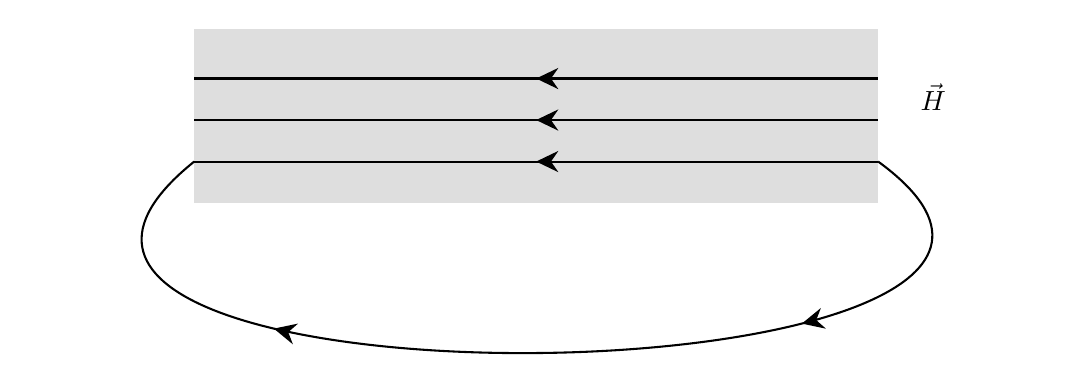
\begin{tikzpicture}[x=0.75pt,y=0.75pt,yscale=-1,xscale=1]
	%uncomment if require: \path (0,300); %set diagram left start at 0, and has height of 300

	%Shape: Rectangle [id:dp5907061259874049] 
	\draw  [draw opacity=0][fill={rgb, 255:red, 222; green, 222; blue, 222 }  ,fill opacity=1 ] (141,93) -- (470.5,93) -- (470.5,177) -- (141,177) -- cycle ;
	%Straight Lines [id:da1873021714837242] 
	\draw    (141,157) -- (470.5,157) ;
	\draw [shift={(305.75,157)}, rotate = 0] [fill={rgb, 255:red, 0; green, 0; blue, 0 }  ][line width=0.08]  [draw opacity=0] (10.72,-5.15) -- (0,0) -- (10.72,5.15) -- (7.12,0) -- cycle    ;
	%Straight Lines [id:da1093458697246743] 
	\draw    (141,137) -- (470.5,137) ;
	\draw [shift={(305.75,137)}, rotate = 0] [fill={rgb, 255:red, 0; green, 0; blue, 0 }  ][line width=0.08]  [draw opacity=0] (10.72,-5.15) -- (0,0) -- (10.72,5.15) -- (7.12,0) -- cycle    ;
	%Straight Lines [id:da18072749408234423] 
	\draw    (141,117) -- (470.5,117) ;
	\draw [shift={(305.75,117)}, rotate = 0] [fill={rgb, 255:red, 0; green, 0; blue, 0 }  ][line width=0.08]  [draw opacity=0] (10.72,-5.15) -- (0,0) -- (10.72,5.15) -- (7.12,0) -- cycle    ;
	%Curve Lines [id:da45159147701622504] 
	\draw    (141,157) .. controls (61.25,221) and (184.13,250.5) .. (306.69,249.25) .. controls (429.25,248) and (551.5,216) .. (470.5,157) ;
	\draw [shift={(179.37,237.49)}, rotate = 13.92] [fill={rgb, 255:red, 0; green, 0; blue, 0 }  ][line width=0.08]  [draw opacity=0] (10.72,-5.15) -- (0,0) -- (10.72,5.15) -- (7.12,0) -- cycle    ;
	\draw [shift={(433.74,235.07)}, rotate = 346.32] [fill={rgb, 255:red, 0; green, 0; blue, 0 }  ][line width=0.08]  [draw opacity=0] (10.72,-5.15) -- (0,0) -- (10.72,5.15) -- (7.12,0) -- cycle    ;

	% Text Node
	\draw (497,126) node    {$\vec{H}$};

	\end{tikzpicture}
\end{figure}
\FloatBarrier

Possiamo applicare le tecniche conosciute per il campo elettrico al calcolo dei campi magnetici, perché le equazioni di partenza sono identiche.

\section{Condizioni al contorno per B e H}

Consideriamo il caso di una superficie di separazione $\Sigma$ fra materiali dia o para magnetici. Supporremo che sulla superficie possa scorrere una corrente superficiale diretta in modo da uscire dal piano del foglio. Supporremo che le costanti $\mu_r$ siano definite.

\begin{figure}[htpb]
	\centering

	\tikzset{every picture/.style={line width=0.75pt}} %set default line width to 0.75pt        

	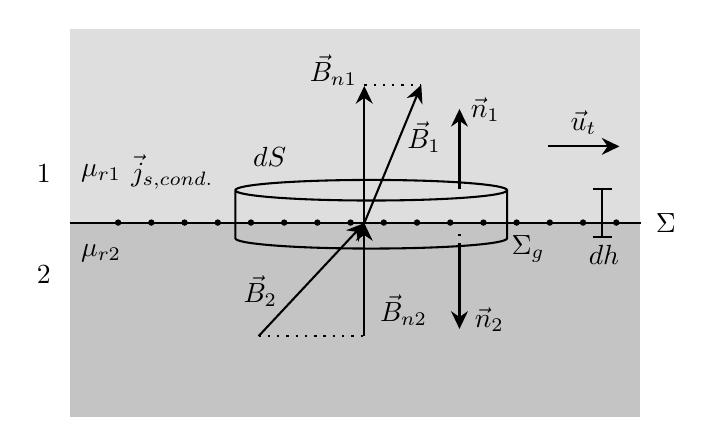
\begin{tikzpicture}[x=0.75pt,y=0.75pt,yscale=-0.8,xscale=0.8]
	%uncomment if require: \path (0,300); %set diagram left start at 0, and has height of 300

	%Shape: Rectangle [id:dp640128671583652] 
	\draw  [draw opacity=0][fill={rgb, 255:red, 222; green, 222; blue, 222 }  ,fill opacity=1 ] (127.5,38) -- (471.33,38) -- (471.33,155) -- (127.5,155) -- cycle ;
	%Shape: Rectangle [id:dp7767382783137311] 
	\draw  [draw opacity=0][fill={rgb, 255:red, 196; green, 196; blue, 196 }  ,fill opacity=1 ] (127.5,155) -- (471.33,155) -- (471.33,272) -- (127.5,272) -- cycle ;
	%Straight Lines [id:da3379231931271103] 
	\draw    (448.33,163.7) -- (448.33,134.5) ;
	\draw [shift={(448.33,134.5)}, rotate = 450] [color={rgb, 255:red, 0; green, 0; blue, 0 }  ][line width=0.75]    (0,5.59) -- (0,-5.59)   ;
	\draw [shift={(448.33,163.7)}, rotate = 450] [color={rgb, 255:red, 0; green, 0; blue, 0 }  ][line width=0.75]    (0,5.59) -- (0,-5.59)   ;
	%Straight Lines [id:da5256110536070768] 
	\draw    (127.5,155) -- (471.5,155) ;
	%Straight Lines [id:da2917764907431699] 
	\draw    (304.99,155.11) -- (338.19,74.61) ;
	\draw [shift={(339.33,71.83)}, rotate = 472.41] [fill={rgb, 255:red, 0; green, 0; blue, 0 }  ][line width=0.08]  [draw opacity=0] (10.72,-5.15) -- (0,0) -- (10.72,5.15) -- (7.12,0) -- cycle    ;
	%Straight Lines [id:da3617226558964304] 
	\draw    (241.33,223.17) -- (302.94,157.3) ;
	\draw [shift={(304.99,155.11)}, rotate = 493.09] [fill={rgb, 255:red, 0; green, 0; blue, 0 }  ][line width=0.08]  [draw opacity=0] (10.72,-5.15) -- (0,0) -- (10.72,5.15) -- (7.12,0) -- cycle    ;
	%Straight Lines [id:da48067503289628477] 
	\draw    (415.66,108.87) -- (455.67,108.87) ;
	\draw [shift={(458.67,108.87)}, rotate = 180] [fill={rgb, 255:red, 0; green, 0; blue, 0 }  ][line width=0.08]  [draw opacity=0] (10.72,-5.15) -- (0,0) -- (10.72,5.15) -- (7.12,0) -- cycle    ;
	%Straight Lines [id:da489443582876224] 
	\draw    (304.99,155.11) -- (304.99,75.5) ;
	\draw [shift={(304.99,72.5)}, rotate = 450] [fill={rgb, 255:red, 0; green, 0; blue, 0 }  ][line width=0.08]  [draw opacity=0] (10.72,-5.15) -- (0,0) -- (10.72,5.15) -- (7.12,0) -- cycle    ;
	%Straight Lines [id:da7541095946452916] 
	\draw  [dash pattern={on 0.84pt off 2.51pt}]  (304.99,71.83) -- (339.33,71.83) ;
	%Straight Lines [id:da29810868951967096] 
	\draw  [dash pattern={on 0.84pt off 2.51pt}]  (241.33,223.17) -- (304.99,223.17) ;
	%Shape: Can [id:dp9154320986569371] 
	\draw   (391,135.27) -- (391,164.2) .. controls (391,167.62) and (354.36,170.4) .. (309.17,170.4) .. controls (263.97,170.4) and (227.33,167.62) .. (227.33,164.2) -- (227.33,135.27) .. controls (227.33,131.84) and (263.97,129.07) .. (309.17,129.07) .. controls (354.36,129.07) and (391,131.84) .. (391,135.27) .. controls (391,138.69) and (354.36,141.47) .. (309.17,141.47) .. controls (263.97,141.47) and (227.33,138.69) .. (227.33,135.27) ;
	%Straight Lines [id:da3186356193706956] 
	\draw    (362.33,134.77) -- (362.33,89.33) ;
	\draw [shift={(362.33,86.33)}, rotate = 450] [fill={rgb, 255:red, 0; green, 0; blue, 0 }  ][line width=0.08]  [draw opacity=0] (10.72,-5.15) -- (0,0) -- (10.72,5.15) -- (7.12,0) -- cycle    ;
	%Straight Lines [id:da7404993802099071] 
	\draw    (362.33,215.77) -- (362.33,168.53) ;
	\draw [shift={(362.33,218.77)}, rotate = 270] [fill={rgb, 255:red, 0; green, 0; blue, 0 }  ][line width=0.08]  [draw opacity=0] (10.72,-5.15) -- (0,0) -- (10.72,5.15) -- (7.12,0) -- cycle    ;
	%Straight Lines [id:da23941741198591937] 
	\draw  [dash pattern={on 0.84pt off 2.51pt}]  (362.33,168.53) -- (362.33,159.53) ;
	%Shape: Circle [id:dp9226117747947826] 
	\draw  [fill={rgb, 255:red, 0; green, 0; blue, 0 }  ,fill opacity=1 ] (155.5,154.75) .. controls (155.5,154.06) and (156.06,153.5) .. (156.75,153.5) .. controls (157.44,153.5) and (158,154.06) .. (158,154.75) .. controls (158,155.44) and (157.44,156) .. (156.75,156) .. controls (156.06,156) and (155.5,155.44) .. (155.5,154.75) -- cycle ;
	%Shape: Circle [id:dp49321895896161183] 
	\draw  [fill={rgb, 255:red, 0; green, 0; blue, 0 }  ,fill opacity=1 ] (175.5,154.75) .. controls (175.5,154.06) and (176.06,153.5) .. (176.75,153.5) .. controls (177.44,153.5) and (178,154.06) .. (178,154.75) .. controls (178,155.44) and (177.44,156) .. (176.75,156) .. controls (176.06,156) and (175.5,155.44) .. (175.5,154.75) -- cycle ;
	%Shape: Circle [id:dp05606420159460934] 
	\draw  [fill={rgb, 255:red, 0; green, 0; blue, 0 }  ,fill opacity=1 ] (195.5,154.75) .. controls (195.5,154.06) and (196.06,153.5) .. (196.75,153.5) .. controls (197.44,153.5) and (198,154.06) .. (198,154.75) .. controls (198,155.44) and (197.44,156) .. (196.75,156) .. controls (196.06,156) and (195.5,155.44) .. (195.5,154.75) -- cycle ;
	%Shape: Circle [id:dp15915469483255507] 
	\draw  [fill={rgb, 255:red, 0; green, 0; blue, 0 }  ,fill opacity=1 ] (215.5,154.75) .. controls (215.5,154.06) and (216.06,153.5) .. (216.75,153.5) .. controls (217.44,153.5) and (218,154.06) .. (218,154.75) .. controls (218,155.44) and (217.44,156) .. (216.75,156) .. controls (216.06,156) and (215.5,155.44) .. (215.5,154.75) -- cycle ;
	%Shape: Circle [id:dp981414568315562] 
	\draw  [fill={rgb, 255:red, 0; green, 0; blue, 0 }  ,fill opacity=1 ] (235.5,154.75) .. controls (235.5,154.06) and (236.06,153.5) .. (236.75,153.5) .. controls (237.44,153.5) and (238,154.06) .. (238,154.75) .. controls (238,155.44) and (237.44,156) .. (236.75,156) .. controls (236.06,156) and (235.5,155.44) .. (235.5,154.75) -- cycle ;
	%Shape: Circle [id:dp8020916372170195] 
	\draw  [fill={rgb, 255:red, 0; green, 0; blue, 0 }  ,fill opacity=1 ] (255.5,154.75) .. controls (255.5,154.06) and (256.06,153.5) .. (256.75,153.5) .. controls (257.44,153.5) and (258,154.06) .. (258,154.75) .. controls (258,155.44) and (257.44,156) .. (256.75,156) .. controls (256.06,156) and (255.5,155.44) .. (255.5,154.75) -- cycle ;
	%Shape: Circle [id:dp9837915663115668] 
	\draw  [fill={rgb, 255:red, 0; green, 0; blue, 0 }  ,fill opacity=1 ] (275.5,154.75) .. controls (275.5,154.06) and (276.06,153.5) .. (276.75,153.5) .. controls (277.44,153.5) and (278,154.06) .. (278,154.75) .. controls (278,155.44) and (277.44,156) .. (276.75,156) .. controls (276.06,156) and (275.5,155.44) .. (275.5,154.75) -- cycle ;
	%Shape: Circle [id:dp7422574202222258] 
	\draw  [fill={rgb, 255:red, 0; green, 0; blue, 0 }  ,fill opacity=1 ] (295.5,154.75) .. controls (295.5,154.06) and (296.06,153.5) .. (296.75,153.5) .. controls (297.44,153.5) and (298,154.06) .. (298,154.75) .. controls (298,155.44) and (297.44,156) .. (296.75,156) .. controls (296.06,156) and (295.5,155.44) .. (295.5,154.75) -- cycle ;
	%Shape: Circle [id:dp962308728843092] 
	\draw  [fill={rgb, 255:red, 0; green, 0; blue, 0 }  ,fill opacity=1 ] (315.5,154.75) .. controls (315.5,154.06) and (316.06,153.5) .. (316.75,153.5) .. controls (317.44,153.5) and (318,154.06) .. (318,154.75) .. controls (318,155.44) and (317.44,156) .. (316.75,156) .. controls (316.06,156) and (315.5,155.44) .. (315.5,154.75) -- cycle ;
	%Shape: Circle [id:dp217945754335507] 
	\draw  [fill={rgb, 255:red, 0; green, 0; blue, 0 }  ,fill opacity=1 ] (335.5,154.75) .. controls (335.5,154.06) and (336.06,153.5) .. (336.75,153.5) .. controls (337.44,153.5) and (338,154.06) .. (338,154.75) .. controls (338,155.44) and (337.44,156) .. (336.75,156) .. controls (336.06,156) and (335.5,155.44) .. (335.5,154.75) -- cycle ;
	%Shape: Circle [id:dp5568851600454661] 
	\draw  [fill={rgb, 255:red, 0; green, 0; blue, 0 }  ,fill opacity=1 ] (355.5,154.75) .. controls (355.5,154.06) and (356.06,153.5) .. (356.75,153.5) .. controls (357.44,153.5) and (358,154.06) .. (358,154.75) .. controls (358,155.44) and (357.44,156) .. (356.75,156) .. controls (356.06,156) and (355.5,155.44) .. (355.5,154.75) -- cycle ;
	%Shape: Circle [id:dp9213331130002607] 
	\draw  [fill={rgb, 255:red, 0; green, 0; blue, 0 }  ,fill opacity=1 ] (375.5,154.75) .. controls (375.5,154.06) and (376.06,153.5) .. (376.75,153.5) .. controls (377.44,153.5) and (378,154.06) .. (378,154.75) .. controls (378,155.44) and (377.44,156) .. (376.75,156) .. controls (376.06,156) and (375.5,155.44) .. (375.5,154.75) -- cycle ;
	%Shape: Circle [id:dp764392096031741] 
	\draw  [fill={rgb, 255:red, 0; green, 0; blue, 0 }  ,fill opacity=1 ] (395.5,154.75) .. controls (395.5,154.06) and (396.06,153.5) .. (396.75,153.5) .. controls (397.44,153.5) and (398,154.06) .. (398,154.75) .. controls (398,155.44) and (397.44,156) .. (396.75,156) .. controls (396.06,156) and (395.5,155.44) .. (395.5,154.75) -- cycle ;
	%Shape: Circle [id:dp053231376142844455] 
	\draw  [fill={rgb, 255:red, 0; green, 0; blue, 0 }  ,fill opacity=1 ] (415.5,154.75) .. controls (415.5,154.06) and (416.06,153.5) .. (416.75,153.5) .. controls (417.44,153.5) and (418,154.06) .. (418,154.75) .. controls (418,155.44) and (417.44,156) .. (416.75,156) .. controls (416.06,156) and (415.5,155.44) .. (415.5,154.75) -- cycle ;
	%Shape: Circle [id:dp5881828482322411] 
	\draw  [fill={rgb, 255:red, 0; green, 0; blue, 0 }  ,fill opacity=1 ] (435.5,154.75) .. controls (435.5,154.06) and (436.06,153.5) .. (436.75,153.5) .. controls (437.44,153.5) and (438,154.06) .. (438,154.75) .. controls (438,155.44) and (437.44,156) .. (436.75,156) .. controls (436.06,156) and (435.5,155.44) .. (435.5,154.75) -- cycle ;
	%Shape: Circle [id:dp029196096719917852] 
	\draw  [fill={rgb, 255:red, 0; green, 0; blue, 0 }  ,fill opacity=1 ] (455.5,154.75) .. controls (455.5,154.06) and (456.06,153.5) .. (456.75,153.5) .. controls (457.44,153.5) and (458,154.06) .. (458,154.75) .. controls (458,155.44) and (457.44,156) .. (456.75,156) .. controls (456.06,156) and (455.5,155.44) .. (455.5,154.75) -- cycle ;
	%Straight Lines [id:da9185749469986559] 
	\draw    (304.99,158.11) -- (304.99,223.17) ;
	\draw [shift={(304.99,155.11)}, rotate = 90] [fill={rgb, 255:red, 0; green, 0; blue, 0 }  ][line width=0.08]  [draw opacity=0] (10.72,-5.15) -- (0,0) -- (10.72,5.15) -- (7.12,0) -- cycle    ;

	% Text Node
	\draw (449.33,174.07) node    {$dh$};
	% Text Node
	\draw (403.67,170.67) node    {$\Sigma _{g}$};
	% Text Node
	\draw (112,125) node    {$1$};
	% Text Node
	\draw (112,186) node    {$2$};
	% Text Node
	\draw (341,103.33) node    {$\vec{B}_{1}$};
	% Text Node
	\draw (242.33,196) node    {$\vec{B}_{2}$};
	% Text Node
	\draw (486.67,155) node    {$\Sigma $};
	% Text Node
	\draw (437,94.77) node    {$\vec{u}_{t}$};
	% Text Node
	\draw (146.5,125) node    {$\mu _{r1}$};
	% Text Node
	\draw (146.5,173.33) node    {$\mu _{r2}$};
	% Text Node
	\draw (286.47,63.07) node    {$\vec{B}_{n1}$};
	% Text Node
	\draw (328.67,207.4) node    {$\vec{B}_{n2}$};
	% Text Node
	\draw (377.93,86.87) node    {$\vec{n}_{1}$};
	% Text Node
	\draw (380.33,213.33) node    {$\vec{n}_{2}$};
	% Text Node
	\draw (248,115.33) node    {$dS$};
	% Text Node
	\draw (189.5,124.33) node    {$\vec{j}_{s,cond.}$};

	\end{tikzpicture}
\end{figure}
\FloatBarrier

Consideriamo una superficie cilindrica a cavallo della superficie e applichiamo il teorema di Gauss ad essa.

\begin{gather*}
	\text{div}\vec{B} =0 \implies \Phi_{\Sigma_g}(\vec{B} )=0 \qquad \sqrt{dS} \gg dh \\
	0=\Phi_{\Sigma_g}(\vec{B} ) \sim \vec{B}_1 \cdot \vec{n}_1\,dS + \vec{B}_2 \cdot \vec{n}_2\,dS = \vec{B}_1 \cdot \vec{n}_1\,dS - \vec{B}_2 \cdot \vec{n}_1\,dS
\end{gather*}

Possiamo chiamare

\begin{gather*}
	B_{1n}=\vec{B}_1\cdot \vec{n}_1\\
	B_{2n}=\vec{B}_2\cdot \vec{n}_1
\end{gather*}

Allora avremo

\[
	B_{1n}-B_{2n}=0 \implies \boxed{B_{1n}=B_{2n}}
\]

Anche in questo caso la componente normale di $\vec{B}$ rispetto alla superficie di separazione si conserva. Vediamo che cosa accade ad $\vec{H}$. Conosciamo la legge che lega $\vec{B}$ ed $\vec{H}$.

\[
	\mu_0 \mu_{r1} H_{1n} = \mu_0 \mu_{r2} H_{2n} \implies \boxed{\mu_{r1} H_{1n} = \mu_{r2} H_{2n}}
\]

Consideriamo a questo punto un percorso chiuso $\gamma$ rettangolare a cavallo delle superfici.

\begin{figure}[htpb]
	\centering

	\tikzset{every picture/.style={line width=0.75pt}} %set default line width to 0.75pt        

	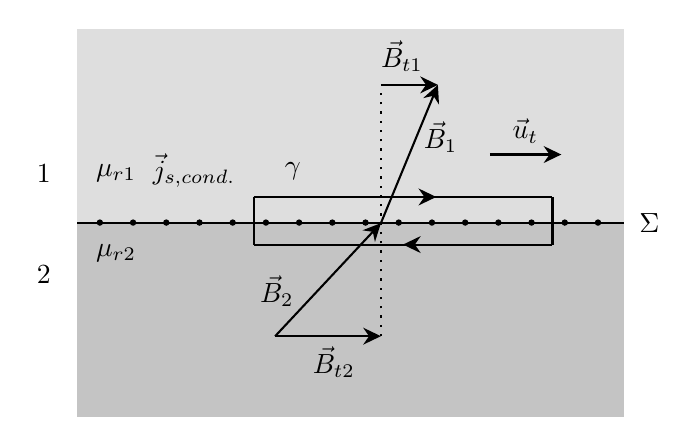
\begin{tikzpicture}[x=0.75pt,y=0.75pt,yscale=-0.8,xscale=0.8]
	%uncomment if require: \path (0,300); %set diagram left start at 0, and has height of 300

	%Shape: Rectangle [id:dp8889811844496274] 
	\draw  [draw opacity=0][fill={rgb, 255:red, 196; green, 196; blue, 196 }  ,fill opacity=1 ] (154,161) -- (483.33,161) -- (483.33,278) -- (154,278) -- cycle ;
	%Shape: Rectangle [id:dp8154040016170578] 
	\draw  [draw opacity=0][fill={rgb, 255:red, 222; green, 222; blue, 222 }  ,fill opacity=1 ] (154,44) -- (483.33,44) -- (483.33,161) -- (154,161) -- cycle ;
	%Straight Lines [id:da9217572029779877] 
	\draw    (154,161) -- (483.5,161) ;
	%Straight Lines [id:da25473814943791107] 
	\draw    (336.99,161.11) -- (370.19,80.61) ;
	\draw [shift={(371.33,77.83)}, rotate = 472.41] [fill={rgb, 255:red, 0; green, 0; blue, 0 }  ][line width=0.08]  [draw opacity=0] (10.72,-5.15) -- (0,0) -- (10.72,5.15) -- (7.12,0) -- cycle    ;
	%Straight Lines [id:da49271486183733937] 
	\draw    (273.33,229.17) -- (334.94,163.3) ;
	\draw [shift={(336.99,161.11)}, rotate = 493.09] [fill={rgb, 255:red, 0; green, 0; blue, 0 }  ][line width=0.08]  [draw opacity=0] (10.72,-5.15) -- (0,0) -- (10.72,5.15) -- (7.12,0) -- cycle    ;
	%Straight Lines [id:da5567500542194554] 
	\draw    (300.33,145.33) -- (440.33,145.33) ;
	\draw [shift={(370.33,145.33)}, rotate = 180] [fill={rgb, 255:red, 0; green, 0; blue, 0 }  ][line width=0.08]  [draw opacity=0] (10.72,-5.15) -- (0,0) -- (10.72,5.15) -- (7.12,0) -- cycle    ;
	%Straight Lines [id:da5436907378732236] 
	\draw    (260.33,174) -- (440.33,174) ;
	\draw [shift={(350.33,174)}, rotate = 0] [fill={rgb, 255:red, 0; green, 0; blue, 0 }  ][line width=0.08]  [draw opacity=0] (10.72,-5.15) -- (0,0) -- (10.72,5.15) -- (7.12,0) -- cycle    ;
	%Straight Lines [id:da10143937001629277] 
	\draw    (440.33,145.33) -- (440.33,174) ;
	%Straight Lines [id:da08569580649940645] 
	\draw    (260.33,145.33) -- (260.33,174) ;
	%Straight Lines [id:da7138367568727535] 
	\draw    (402.66,119.77) -- (442.67,119.77) ;
	\draw [shift={(445.67,119.77)}, rotate = 180] [fill={rgb, 255:red, 0; green, 0; blue, 0 }  ][line width=0.08]  [draw opacity=0] (10.72,-5.15) -- (0,0) -- (10.72,5.15) -- (7.12,0) -- cycle    ;
	%Straight Lines [id:da05949564858271583] 
	\draw  [dash pattern={on 0.84pt off 2.51pt}]  (336.99,229.17) -- (336.99,78.5) ;
	%Straight Lines [id:da5732763015102671] 
	\draw    (336.99,77.83) -- (368.33,77.83) ;
	\draw [shift={(371.33,77.83)}, rotate = 180] [fill={rgb, 255:red, 0; green, 0; blue, 0 }  ][line width=0.08]  [draw opacity=0] (10.72,-5.15) -- (0,0) -- (10.72,5.15) -- (7.12,0) -- cycle    ;
	%Straight Lines [id:da4618494416402683] 
	\draw    (273.33,229.17) -- (333.99,229.17) ;
	\draw [shift={(336.99,229.17)}, rotate = 180] [fill={rgb, 255:red, 0; green, 0; blue, 0 }  ][line width=0.08]  [draw opacity=0] (10.72,-5.15) -- (0,0) -- (10.72,5.15) -- (7.12,0) -- cycle    ;
	%Shape: Circle [id:dp46729674948235456] 
	\draw  [fill={rgb, 255:red, 0; green, 0; blue, 0 }  ,fill opacity=1 ] (166.5,160.75) .. controls (166.5,160.06) and (167.06,159.5) .. (167.75,159.5) .. controls (168.44,159.5) and (169,160.06) .. (169,160.75) .. controls (169,161.44) and (168.44,162) .. (167.75,162) .. controls (167.06,162) and (166.5,161.44) .. (166.5,160.75) -- cycle ;
	%Shape: Circle [id:dp8132634527969875] 
	\draw  [fill={rgb, 255:red, 0; green, 0; blue, 0 }  ,fill opacity=1 ] (186.5,160.75) .. controls (186.5,160.06) and (187.06,159.5) .. (187.75,159.5) .. controls (188.44,159.5) and (189,160.06) .. (189,160.75) .. controls (189,161.44) and (188.44,162) .. (187.75,162) .. controls (187.06,162) and (186.5,161.44) .. (186.5,160.75) -- cycle ;
	%Shape: Circle [id:dp8025783798209374] 
	\draw  [fill={rgb, 255:red, 0; green, 0; blue, 0 }  ,fill opacity=1 ] (206.5,160.75) .. controls (206.5,160.06) and (207.06,159.5) .. (207.75,159.5) .. controls (208.44,159.5) and (209,160.06) .. (209,160.75) .. controls (209,161.44) and (208.44,162) .. (207.75,162) .. controls (207.06,162) and (206.5,161.44) .. (206.5,160.75) -- cycle ;
	%Shape: Circle [id:dp25029115254588685] 
	\draw  [fill={rgb, 255:red, 0; green, 0; blue, 0 }  ,fill opacity=1 ] (226.5,160.75) .. controls (226.5,160.06) and (227.06,159.5) .. (227.75,159.5) .. controls (228.44,159.5) and (229,160.06) .. (229,160.75) .. controls (229,161.44) and (228.44,162) .. (227.75,162) .. controls (227.06,162) and (226.5,161.44) .. (226.5,160.75) -- cycle ;
	%Shape: Circle [id:dp5547302977144766] 
	\draw  [fill={rgb, 255:red, 0; green, 0; blue, 0 }  ,fill opacity=1 ] (246.5,160.75) .. controls (246.5,160.06) and (247.06,159.5) .. (247.75,159.5) .. controls (248.44,159.5) and (249,160.06) .. (249,160.75) .. controls (249,161.44) and (248.44,162) .. (247.75,162) .. controls (247.06,162) and (246.5,161.44) .. (246.5,160.75) -- cycle ;
	%Shape: Circle [id:dp33969588247409366] 
	\draw  [fill={rgb, 255:red, 0; green, 0; blue, 0 }  ,fill opacity=1 ] (266.5,160.75) .. controls (266.5,160.06) and (267.06,159.5) .. (267.75,159.5) .. controls (268.44,159.5) and (269,160.06) .. (269,160.75) .. controls (269,161.44) and (268.44,162) .. (267.75,162) .. controls (267.06,162) and (266.5,161.44) .. (266.5,160.75) -- cycle ;
	%Shape: Circle [id:dp6564194490201183] 
	\draw  [fill={rgb, 255:red, 0; green, 0; blue, 0 }  ,fill opacity=1 ] (286.5,160.75) .. controls (286.5,160.06) and (287.06,159.5) .. (287.75,159.5) .. controls (288.44,159.5) and (289,160.06) .. (289,160.75) .. controls (289,161.44) and (288.44,162) .. (287.75,162) .. controls (287.06,162) and (286.5,161.44) .. (286.5,160.75) -- cycle ;
	%Shape: Circle [id:dp037619467526890604] 
	\draw  [fill={rgb, 255:red, 0; green, 0; blue, 0 }  ,fill opacity=1 ] (306.5,160.75) .. controls (306.5,160.06) and (307.06,159.5) .. (307.75,159.5) .. controls (308.44,159.5) and (309,160.06) .. (309,160.75) .. controls (309,161.44) and (308.44,162) .. (307.75,162) .. controls (307.06,162) and (306.5,161.44) .. (306.5,160.75) -- cycle ;
	%Shape: Circle [id:dp9895523027397202] 
	\draw  [fill={rgb, 255:red, 0; green, 0; blue, 0 }  ,fill opacity=1 ] (326.5,160.75) .. controls (326.5,160.06) and (327.06,159.5) .. (327.75,159.5) .. controls (328.44,159.5) and (329,160.06) .. (329,160.75) .. controls (329,161.44) and (328.44,162) .. (327.75,162) .. controls (327.06,162) and (326.5,161.44) .. (326.5,160.75) -- cycle ;
	%Shape: Circle [id:dp5800186845267619] 
	\draw  [fill={rgb, 255:red, 0; green, 0; blue, 0 }  ,fill opacity=1 ] (346.5,160.75) .. controls (346.5,160.06) and (347.06,159.5) .. (347.75,159.5) .. controls (348.44,159.5) and (349,160.06) .. (349,160.75) .. controls (349,161.44) and (348.44,162) .. (347.75,162) .. controls (347.06,162) and (346.5,161.44) .. (346.5,160.75) -- cycle ;
	%Shape: Circle [id:dp6910511077291763] 
	\draw  [fill={rgb, 255:red, 0; green, 0; blue, 0 }  ,fill opacity=1 ] (366.5,160.75) .. controls (366.5,160.06) and (367.06,159.5) .. (367.75,159.5) .. controls (368.44,159.5) and (369,160.06) .. (369,160.75) .. controls (369,161.44) and (368.44,162) .. (367.75,162) .. controls (367.06,162) and (366.5,161.44) .. (366.5,160.75) -- cycle ;
	%Shape: Circle [id:dp9964405128303655] 
	\draw  [fill={rgb, 255:red, 0; green, 0; blue, 0 }  ,fill opacity=1 ] (386.5,160.75) .. controls (386.5,160.06) and (387.06,159.5) .. (387.75,159.5) .. controls (388.44,159.5) and (389,160.06) .. (389,160.75) .. controls (389,161.44) and (388.44,162) .. (387.75,162) .. controls (387.06,162) and (386.5,161.44) .. (386.5,160.75) -- cycle ;
	%Shape: Circle [id:dp31251253187467376] 
	\draw  [fill={rgb, 255:red, 0; green, 0; blue, 0 }  ,fill opacity=1 ] (406.5,160.75) .. controls (406.5,160.06) and (407.06,159.5) .. (407.75,159.5) .. controls (408.44,159.5) and (409,160.06) .. (409,160.75) .. controls (409,161.44) and (408.44,162) .. (407.75,162) .. controls (407.06,162) and (406.5,161.44) .. (406.5,160.75) -- cycle ;
	%Shape: Circle [id:dp8429011669329816] 
	\draw  [fill={rgb, 255:red, 0; green, 0; blue, 0 }  ,fill opacity=1 ] (426.5,160.75) .. controls (426.5,160.06) and (427.06,159.5) .. (427.75,159.5) .. controls (428.44,159.5) and (429,160.06) .. (429,160.75) .. controls (429,161.44) and (428.44,162) .. (427.75,162) .. controls (427.06,162) and (426.5,161.44) .. (426.5,160.75) -- cycle ;
	%Shape: Circle [id:dp575471172390928] 
	\draw  [fill={rgb, 255:red, 0; green, 0; blue, 0 }  ,fill opacity=1 ] (446.5,160.75) .. controls (446.5,160.06) and (447.06,159.5) .. (447.75,159.5) .. controls (448.44,159.5) and (449,160.06) .. (449,160.75) .. controls (449,161.44) and (448.44,162) .. (447.75,162) .. controls (447.06,162) and (446.5,161.44) .. (446.5,160.75) -- cycle ;
	%Shape: Circle [id:dp6087226715450742] 
	\draw  [fill={rgb, 255:red, 0; green, 0; blue, 0 }  ,fill opacity=1 ] (466.5,160.75) .. controls (466.5,160.06) and (467.06,159.5) .. (467.75,159.5) .. controls (468.44,159.5) and (469,160.06) .. (469,160.75) .. controls (469,161.44) and (468.44,162) .. (467.75,162) .. controls (467.06,162) and (466.5,161.44) .. (466.5,160.75) -- cycle ;
	%Straight Lines [id:da9848989975392397] 
	\draw    (260.33,145.33) -- (300.33,145.33) ;

	% Text Node
	\draw (134,131) node    {$1$};
	% Text Node
	\draw (134,192) node    {$2$};
	% Text Node
	\draw (373,109.33) node    {$\vec{B}_{1}$};
	% Text Node
	\draw (274.33,202) node    {$\vec{B}_{2}$};
	% Text Node
	\draw (498.67,161) node    {$\Sigma $};
	% Text Node
	\draw (424,105.67) node    {$\vec{u}_{t}$};
	% Text Node
	\draw (284,130) node    {$\gamma $};
	% Text Node
	\draw (224.5,129.33) node    {$\vec{j}_{s,cond.}$};
	% Text Node
	\draw (177.5,131) node    {$\mu _{r1}$};
	% Text Node
	\draw (177.5,179.33) node    {$\mu _{r2}$};
	% Text Node
	\draw (349.67,60.67) node    {$\vec{B}_{t1}$};
	% Text Node
	\draw (308.67,245) node    {$\vec{B}_{t2}$};

	\end{tikzpicture}
\end{figure}
\FloatBarrier

Siamo interessati alla componente tangente quindi dobbiamo applicare la legge di Ampere:

\begin{gather*}
	\oint_{\gamma} \vec{H} \cdot d\vec{l} = I_{\text{conduzione}}^{\text{conc. a}\gamma} \qquad dh \ll dl \\
	\vec{H}_1\cdot dl\,\vec{u}_t - \vec{H}_2\cdot dl\,\vec{u}_t =j^{\text{cond.}} dl \implies \boxed{H_{1t}-H_{2t}=j^{\text{cond.}}}
\end{gather*}

Possiamo ricavare cosa succede alla componente tangente di $\vec{B}$:

\[
	\frac{B_{1t}}{\mu_0 \mu_{r1}} - \frac{B_{2t}}{\mu_0 \mu_{r2}} = j^{\text{cond.}}  \implies \boxed{\frac{B_{1t}}{\mu_{r1}} - \frac{B_{2t}}{\mu_{r2}} = \mu_0 \,j^{\text{cond.}}}
\]

Le correnti di magnetizzazione concorrono ai campi magnetici. Avendo due mezzi diversi ci saranno correnti di magnetizzazione superficiali.